\documentclass{article} % For LaTeX2e
\usepackage{iclr2027_conference,times}

% Optional math commands from https://github.com/goodfeli/dlbook_notation.
%%%%% NEW MATH DEFINITIONS %%%%%

\usepackage{amsmath,amsfonts,bm}

% Mark sections of captions for referring to divisions of figures
\newcommand{\figleft}{{\em (Left)}}
\newcommand{\figcenter}{{\em (Center)}}
\newcommand{\figright}{{\em (Right)}}
\newcommand{\figtop}{{\em (Top)}}
\newcommand{\figbottom}{{\em (Bottom)}}
\newcommand{\captiona}{{\em (a)}}
\newcommand{\captionb}{{\em (b)}}
\newcommand{\captionc}{{\em (c)}}
\newcommand{\captiond}{{\em (d)}}

% Highlight a newly defined term
\newcommand{\newterm}[1]{{\bf #1}}


% Figure reference, lower-case.
\def\figref#1{figure~\ref{#1}}
% Figure reference, capital. For start of sentence
\def\Figref#1{Figure~\ref{#1}}
\def\twofigref#1#2{figures \ref{#1} and \ref{#2}}
\def\quadfigref#1#2#3#4{figures \ref{#1}, \ref{#2}, \ref{#3} and \ref{#4}}
% Section reference, lower-case.
\def\secref#1{section~\ref{#1}}
% Section reference, capital.
\def\Secref#1{Section~\ref{#1}}
% Reference to two sections.
\def\twosecrefs#1#2{sections \ref{#1} and \ref{#2}}
% Reference to three sections.
\def\secrefs#1#2#3{sections \ref{#1}, \ref{#2} and \ref{#3}}
% Reference to an equation, lower-case.
\def\eqref#1{equation~\ref{#1}}
% Reference to an equation, upper case
\def\Eqref#1{Equation~\ref{#1}}
% A raw reference to an equation---avoid using if possible
\def\plaineqref#1{\ref{#1}}
% Reference to a chapter, lower-case.
\def\chapref#1{chapter~\ref{#1}}
% Reference to an equation, upper case.
\def\Chapref#1{Chapter~\ref{#1}}
% Reference to a range of chapters
\def\rangechapref#1#2{chapters\ref{#1}--\ref{#2}}
% Reference to an algorithm, lower-case.
\def\algref#1{algorithm~\ref{#1}}
% Reference to an algorithm, upper case.
\def\Algref#1{Algorithm~\ref{#1}}
\def\twoalgref#1#2{algorithms \ref{#1} and \ref{#2}}
\def\Twoalgref#1#2{Algorithms \ref{#1} and \ref{#2}}
% Reference to a part, lower case
\def\partref#1{part~\ref{#1}}
% Reference to a part, upper case
\def\Partref#1{Part~\ref{#1}}
\def\twopartref#1#2{parts \ref{#1} and \ref{#2}}

\def\ceil#1{\lceil #1 \rceil}
\def\floor#1{\lfloor #1 \rfloor}
\def\1{\bm{1}}
\newcommand{\train}{\mathcal{D}}
\newcommand{\valid}{\mathcal{D_{\mathrm{valid}}}}
\newcommand{\test}{\mathcal{D_{\mathrm{test}}}}

\def\eps{{\epsilon}}


% Random variables
\def\reta{{\textnormal{$\eta$}}}
\def\ra{{\textnormal{a}}}
\def\rb{{\textnormal{b}}}
\def\rc{{\textnormal{c}}}
\def\rd{{\textnormal{d}}}
\def\re{{\textnormal{e}}}
\def\rf{{\textnormal{f}}}
\def\rg{{\textnormal{g}}}
\def\rh{{\textnormal{h}}}
\def\ri{{\textnormal{i}}}
\def\rj{{\textnormal{j}}}
\def\rk{{\textnormal{k}}}
\def\rl{{\textnormal{l}}}
% rm is already a command, just don't name any random variables m
\def\rn{{\textnormal{n}}}
\def\ro{{\textnormal{o}}}
\def\rp{{\textnormal{p}}}
\def\rq{{\textnormal{q}}}
\def\rr{{\textnormal{r}}}
\def\rs{{\textnormal{s}}}
\def\rt{{\textnormal{t}}}
\def\ru{{\textnormal{u}}}
\def\rv{{\textnormal{v}}}
\def\rw{{\textnormal{w}}}
\def\rx{{\textnormal{x}}}
\def\ry{{\textnormal{y}}}
\def\rz{{\textnormal{z}}}

% Random vectors
\def\rvepsilon{{\mathbf{\epsilon}}}
\def\rvtheta{{\mathbf{\theta}}}
\def\rva{{\mathbf{a}}}
\def\rvb{{\mathbf{b}}}
\def\rvc{{\mathbf{c}}}
\def\rvd{{\mathbf{d}}}
\def\rve{{\mathbf{e}}}
\def\rvf{{\mathbf{f}}}
\def\rvg{{\mathbf{g}}}
\def\rvh{{\mathbf{h}}}
\def\rvu{{\mathbf{i}}}
\def\rvj{{\mathbf{j}}}
\def\rvk{{\mathbf{k}}}
\def\rvl{{\mathbf{l}}}
\def\rvm{{\mathbf{m}}}
\def\rvn{{\mathbf{n}}}
\def\rvo{{\mathbf{o}}}
\def\rvp{{\mathbf{p}}}
\def\rvq{{\mathbf{q}}}
\def\rvr{{\mathbf{r}}}
\def\rvs{{\mathbf{s}}}
\def\rvt{{\mathbf{t}}}
\def\rvu{{\mathbf{u}}}
\def\rvv{{\mathbf{v}}}
\def\rvw{{\mathbf{w}}}
\def\rvx{{\mathbf{x}}}
\def\rvy{{\mathbf{y}}}
\def\rvz{{\mathbf{z}}}

% Elements of random vectors
\def\erva{{\textnormal{a}}}
\def\ervb{{\textnormal{b}}}
\def\ervc{{\textnormal{c}}}
\def\ervd{{\textnormal{d}}}
\def\erve{{\textnormal{e}}}
\def\ervf{{\textnormal{f}}}
\def\ervg{{\textnormal{g}}}
\def\ervh{{\textnormal{h}}}
\def\ervi{{\textnormal{i}}}
\def\ervj{{\textnormal{j}}}
\def\ervk{{\textnormal{k}}}
\def\ervl{{\textnormal{l}}}
\def\ervm{{\textnormal{m}}}
\def\ervn{{\textnormal{n}}}
\def\ervo{{\textnormal{o}}}
\def\ervp{{\textnormal{p}}}
\def\ervq{{\textnormal{q}}}
\def\ervr{{\textnormal{r}}}
\def\ervs{{\textnormal{s}}}
\def\ervt{{\textnormal{t}}}
\def\ervu{{\textnormal{u}}}
\def\ervv{{\textnormal{v}}}
\def\ervw{{\textnormal{w}}}
\def\ervx{{\textnormal{x}}}
\def\ervy{{\textnormal{y}}}
\def\ervz{{\textnormal{z}}}

% Random matrices
\def\rmA{{\mathbf{A}}}
\def\rmB{{\mathbf{B}}}
\def\rmC{{\mathbf{C}}}
\def\rmD{{\mathbf{D}}}
\def\rmE{{\mathbf{E}}}
\def\rmF{{\mathbf{F}}}
\def\rmG{{\mathbf{G}}}
\def\rmH{{\mathbf{H}}}
\def\rmI{{\mathbf{I}}}
\def\rmJ{{\mathbf{J}}}
\def\rmK{{\mathbf{K}}}
\def\rmL{{\mathbf{L}}}
\def\rmM{{\mathbf{M}}}
\def\rmN{{\mathbf{N}}}
\def\rmO{{\mathbf{O}}}
\def\rmP{{\mathbf{P}}}
\def\rmQ{{\mathbf{Q}}}
\def\rmR{{\mathbf{R}}}
\def\rmS{{\mathbf{S}}}
\def\rmT{{\mathbf{T}}}
\def\rmU{{\mathbf{U}}}
\def\rmV{{\mathbf{V}}}
\def\rmW{{\mathbf{W}}}
\def\rmX{{\mathbf{X}}}
\def\rmY{{\mathbf{Y}}}
\def\rmZ{{\mathbf{Z}}}

% Elements of random matrices
\def\ermA{{\textnormal{A}}}
\def\ermB{{\textnormal{B}}}
\def\ermC{{\textnormal{C}}}
\def\ermD{{\textnormal{D}}}
\def\ermE{{\textnormal{E}}}
\def\ermF{{\textnormal{F}}}
\def\ermG{{\textnormal{G}}}
\def\ermH{{\textnormal{H}}}
\def\ermI{{\textnormal{I}}}
\def\ermJ{{\textnormal{J}}}
\def\ermK{{\textnormal{K}}}
\def\ermL{{\textnormal{L}}}
\def\ermM{{\textnormal{M}}}
\def\ermN{{\textnormal{N}}}
\def\ermO{{\textnormal{O}}}
\def\ermP{{\textnormal{P}}}
\def\ermQ{{\textnormal{Q}}}
\def\ermR{{\textnormal{R}}}
\def\ermS{{\textnormal{S}}}
\def\ermT{{\textnormal{T}}}
\def\ermU{{\textnormal{U}}}
\def\ermV{{\textnormal{V}}}
\def\ermW{{\textnormal{W}}}
\def\ermX{{\textnormal{X}}}
\def\ermY{{\textnormal{Y}}}
\def\ermZ{{\textnormal{Z}}}

% Vectors
\def\vzero{{\bm{0}}}
\def\vone{{\bm{1}}}
\def\vmu{{\bm{\mu}}}
\def\vtheta{{\bm{\theta}}}
\def\va{{\bm{a}}}
\def\vb{{\bm{b}}}
\def\vc{{\bm{c}}}
\def\vd{{\bm{d}}}
\def\ve{{\bm{e}}}
\def\vf{{\bm{f}}}
\def\vg{{\bm{g}}}
\def\vh{{\bm{h}}}
\def\vi{{\bm{i}}}
\def\vj{{\bm{j}}}
\def\vk{{\bm{k}}}
\def\vl{{\bm{l}}}
\def\vm{{\bm{m}}}
\def\vn{{\bm{n}}}
\def\vo{{\bm{o}}}
\def\vp{{\bm{p}}}
\def\vq{{\bm{q}}}
\def\vr{{\bm{r}}}
\def\vs{{\bm{s}}}
\def\vt{{\bm{t}}}
\def\vu{{\bm{u}}}
\def\vv{{\bm{v}}}
\def\vw{{\bm{w}}}
\def\vx{{\bm{x}}}
\def\vy{{\bm{y}}}
\def\vz{{\bm{z}}}

% Elements of vectors
\def\evalpha{{\alpha}}
\def\evbeta{{\beta}}
\def\evepsilon{{\epsilon}}
\def\evlambda{{\lambda}}
\def\evomega{{\omega}}
\def\evmu{{\mu}}
\def\evpsi{{\psi}}
\def\evsigma{{\sigma}}
\def\evtheta{{\theta}}
\def\eva{{a}}
\def\evb{{b}}
\def\evc{{c}}
\def\evd{{d}}
\def\eve{{e}}
\def\evf{{f}}
\def\evg{{g}}
\def\evh{{h}}
\def\evi{{i}}
\def\evj{{j}}
\def\evk{{k}}
\def\evl{{l}}
\def\evm{{m}}
\def\evn{{n}}
\def\evo{{o}}
\def\evp{{p}}
\def\evq{{q}}
\def\evr{{r}}
\def\evs{{s}}
\def\evt{{t}}
\def\evu{{u}}
\def\evv{{v}}
\def\evw{{w}}
\def\evx{{x}}
\def\evy{{y}}
\def\evz{{z}}

% Matrix
\def\mA{{\bm{A}}}
\def\mB{{\bm{B}}}
\def\mC{{\bm{C}}}
\def\mD{{\bm{D}}}
\def\mE{{\bm{E}}}
\def\mF{{\bm{F}}}
\def\mG{{\bm{G}}}
\def\mH{{\bm{H}}}
\def\mI{{\bm{I}}}
\def\mJ{{\bm{J}}}
\def\mK{{\bm{K}}}
\def\mL{{\bm{L}}}
\def\mM{{\bm{M}}}
\def\mN{{\bm{N}}}
\def\mO{{\bm{O}}}
\def\mP{{\bm{P}}}
\def\mQ{{\bm{Q}}}
\def\mR{{\bm{R}}}
\def\mS{{\bm{S}}}
\def\mT{{\bm{T}}}
\def\mU{{\bm{U}}}
\def\mV{{\bm{V}}}
\def\mW{{\bm{W}}}
\def\mX{{\bm{X}}}
\def\mY{{\bm{Y}}}
\def\mZ{{\bm{Z}}}
\def\mBeta{{\bm{\beta}}}
\def\mPhi{{\bm{\Phi}}}
\def\mLambda{{\bm{\Lambda}}}
\def\mSigma{{\bm{\Sigma}}}

% Tensor
\DeclareMathAlphabet{\mathsfit}{\encodingdefault}{\sfdefault}{m}{sl}
\SetMathAlphabet{\mathsfit}{bold}{\encodingdefault}{\sfdefault}{bx}{n}
\newcommand{\tens}[1]{\bm{\mathsfit{#1}}}
\def\tA{{\tens{A}}}
\def\tB{{\tens{B}}}
\def\tC{{\tens{C}}}
\def\tD{{\tens{D}}}
\def\tE{{\tens{E}}}
\def\tF{{\tens{F}}}
\def\tG{{\tens{G}}}
\def\tH{{\tens{H}}}
\def\tI{{\tens{I}}}
\def\tJ{{\tens{J}}}
\def\tK{{\tens{K}}}
\def\tL{{\tens{L}}}
\def\tM{{\tens{M}}}
\def\tN{{\tens{N}}}
\def\tO{{\tens{O}}}
\def\tP{{\tens{P}}}
\def\tQ{{\tens{Q}}}
\def\tR{{\tens{R}}}
\def\tS{{\tens{S}}}
\def\tT{{\tens{T}}}
\def\tU{{\tens{U}}}
\def\tV{{\tens{V}}}
\def\tW{{\tens{W}}}
\def\tX{{\tens{X}}}
\def\tY{{\tens{Y}}}
\def\tZ{{\tens{Z}}}


% Graph
\def\gA{{\mathcal{A}}}
\def\gB{{\mathcal{B}}}
\def\gC{{\mathcal{C}}}
\def\gD{{\mathcal{D}}}
\def\gE{{\mathcal{E}}}
\def\gF{{\mathcal{F}}}
\def\gG{{\mathcal{G}}}
\def\gH{{\mathcal{H}}}
\def\gI{{\mathcal{I}}}
\def\gJ{{\mathcal{J}}}
\def\gK{{\mathcal{K}}}
\def\gL{{\mathcal{L}}}
\def\gM{{\mathcal{M}}}
\def\gN{{\mathcal{N}}}
\def\gO{{\mathcal{O}}}
\def\gP{{\mathcal{P}}}
\def\gQ{{\mathcal{Q}}}
\def\gR{{\mathcal{R}}}
\def\gS{{\mathcal{S}}}
\def\gT{{\mathcal{T}}}
\def\gU{{\mathcal{U}}}
\def\gV{{\mathcal{V}}}
\def\gW{{\mathcal{W}}}
\def\gX{{\mathcal{X}}}
\def\gY{{\mathcal{Y}}}
\def\gZ{{\mathcal{Z}}}

% Sets
\def\sA{{\mathbb{A}}}
\def\sB{{\mathbb{B}}}
\def\sC{{\mathbb{C}}}
\def\sD{{\mathbb{D}}}
% Don't use a set called E, because this would be the same as our symbol
% for expectation.
\def\sF{{\mathbb{F}}}
\def\sG{{\mathbb{G}}}
\def\sH{{\mathbb{H}}}
\def\sI{{\mathbb{I}}}
\def\sJ{{\mathbb{J}}}
\def\sK{{\mathbb{K}}}
\def\sL{{\mathbb{L}}}
\def\sM{{\mathbb{M}}}
\def\sN{{\mathbb{N}}}
\def\sO{{\mathbb{O}}}
\def\sP{{\mathbb{P}}}
\def\sQ{{\mathbb{Q}}}
\def\sR{{\mathbb{R}}}
\def\sS{{\mathbb{S}}}
\def\sT{{\mathbb{T}}}
\def\sU{{\mathbb{U}}}
\def\sV{{\mathbb{V}}}
\def\sW{{\mathbb{W}}}
\def\sX{{\mathbb{X}}}
\def\sY{{\mathbb{Y}}}
\def\sZ{{\mathbb{Z}}}

% Entries of a matrix
\def\emLambda{{\Lambda}}
\def\emA{{A}}
\def\emB{{B}}
\def\emC{{C}}
\def\emD{{D}}
\def\emE{{E}}
\def\emF{{F}}
\def\emG{{G}}
\def\emH{{H}}
\def\emI{{I}}
\def\emJ{{J}}
\def\emK{{K}}
\def\emL{{L}}
\def\emM{{M}}
\def\emN{{N}}
\def\emO{{O}}
\def\emP{{P}}
\def\emQ{{Q}}
\def\emR{{R}}
\def\emS{{S}}
\def\emT{{T}}
\def\emU{{U}}
\def\emV{{V}}
\def\emW{{W}}
\def\emX{{X}}
\def\emY{{Y}}
\def\emZ{{Z}}
\def\emSigma{{\Sigma}}

% entries of a tensor
% Same font as tensor, without \bm wrapper
\newcommand{\etens}[1]{\mathsfit{#1}}
\def\etLambda{{\etens{\Lambda}}}
\def\etA{{\etens{A}}}
\def\etB{{\etens{B}}}
\def\etC{{\etens{C}}}
\def\etD{{\etens{D}}}
\def\etE{{\etens{E}}}
\def\etF{{\etens{F}}}
\def\etG{{\etens{G}}}
\def\etH{{\etens{H}}}
\def\etI{{\etens{I}}}
\def\etJ{{\etens{J}}}
\def\etK{{\etens{K}}}
\def\etL{{\etens{L}}}
\def\etM{{\etens{M}}}
\def\etN{{\etens{N}}}
\def\etO{{\etens{O}}}
\def\etP{{\etens{P}}}
\def\etQ{{\etens{Q}}}
\def\etR{{\etens{R}}}
\def\etS{{\etens{S}}}
\def\etT{{\etens{T}}}
\def\etU{{\etens{U}}}
\def\etV{{\etens{V}}}
\def\etW{{\etens{W}}}
\def\etX{{\etens{X}}}
\def\etY{{\etens{Y}}}
\def\etZ{{\etens{Z}}}

% The true underlying data generating distribution
\newcommand{\pdata}{p_{\rm{data}}}
% The empirical distribution defined by the training set
\newcommand{\ptrain}{\hat{p}_{\rm{data}}}
\newcommand{\Ptrain}{\hat{P}_{\rm{data}}}
% The model distribution
\newcommand{\pmodel}{p_{\rm{model}}}
\newcommand{\Pmodel}{P_{\rm{model}}}
\newcommand{\ptildemodel}{\tilde{p}_{\rm{model}}}
% Stochastic autoencoder distributions
\newcommand{\pencode}{p_{\rm{encoder}}}
\newcommand{\pdecode}{p_{\rm{decoder}}}
\newcommand{\precons}{p_{\rm{reconstruct}}}

\newcommand{\laplace}{\mathrm{Laplace}} % Laplace distribution

\newcommand{\E}{\mathbb{E}}
\newcommand{\Ls}{\mathcal{L}}
\newcommand{\R}{\mathbb{R}}
\newcommand{\emp}{\tilde{p}}
\newcommand{\lr}{\alpha}
\newcommand{\reg}{\lambda}
\newcommand{\rect}{\mathrm{rectifier}}
\newcommand{\softmax}{\mathrm{softmax}}
\newcommand{\sigmoid}{\sigma}
\newcommand{\softplus}{\zeta}
\newcommand{\KL}{D_{\mathrm{KL}}}
\newcommand{\Var}{\mathrm{Var}}
\newcommand{\standarderror}{\mathrm{SE}}
\newcommand{\Cov}{\mathrm{Cov}}
% Wolfram Mathworld says $L^2$ is for function spaces and $\ell^2$ is for vectors
% But then they seem to use $L^2$ for vectors throughout the site, and so does
% wikipedia.
\newcommand{\normlzero}{L^0}
\newcommand{\normlone}{L^1}
\newcommand{\normltwo}{L^2}
\newcommand{\normlp}{L^p}
\newcommand{\normmax}{L^\infty}

\newcommand{\parents}{Pa} % See usage in notation.tex. Chosen to match Daphne's book.

\DeclareMathOperator*{\argmax}{arg\,max}
\DeclareMathOperator*{\argmin}{arg\,min}

\DeclareMathOperator{\sign}{sign}
\DeclareMathOperator{\Tr}{Tr}
\let\ab\allowbreak


\usepackage{hyperref}
\usepackage{url}
\usepackage[utf8]{inputenc} % allow utf-8 input
\usepackage[T1]{fontenc}    % use 8-bit T1 fonts
\usepackage{hyperref}       % hyperlinks
\usepackage{url}            % simple URL typesetting
\usepackage{booktabs}       % professional-quality tables
\usepackage{amsfonts}       % blackboard math symbols
\usepackage{nicefrac}       % compact symbols for 1/2, etc.
\usepackage{microtype}      % microtypography
\usepackage{xcolor}         % colors

\usepackage{tabularx}
\usepackage{times}
\usepackage{soul}
\usepackage{caption}
\usepackage{graphicx}
\usepackage{subcaption}
\usepackage{amsmath}
\usepackage{amsthm}
\usepackage{amssymb}
\usepackage{algorithm}
\usepackage{algorithmicx}
\usepackage[noend]{algpseudocode}
\usepackage{multicol}
\usepackage{wrapfig}
\usepackage{multirow}
\usepackage{comment}
\usepackage{tikz}
\usetikzlibrary{positioning,shapes.geometric,shapes.misc,arrows.meta}


\title{Advances in Marginal Inference for\\ Chain-Graph Logical Credal Networks}

% Authors must not appear in the submitted version. They should be hidden
% as long as the \iclrfinalcopy macro remains commented out below.
% Non-anonymous submissions will be rejected without review.

\author{Antiquus S.~Hippocampus, Natalia Cerebro \& Amelie P. Amygdale \thanks{ Use footnote for providing further information
about author (webpage, alternative address)---\emph{not} for acknowledging
funding agencies.  Funding acknowledgements go at the end of the paper.} \\
Department of Computer Science\\
Cranberry-Lemon University\\
Pittsburgh, PA 15213, USA \\
\texttt{\{hippo,brain,jen\}@cs.cranberry-lemon.edu} \\
\And
Ji Q. Ren \& Yevgeny LeNet \\
Department of Computational Neuroscience \\
University of the Witwatersrand \\
Joburg, South Africa \\
\texttt{\{robot,net\}@wits.ac.za} \\
\AND
Coauthor \\
Affiliation \\
Address \\
\texttt{email}
}

% The \author macro works with any number of authors. There are two commands
% used to separate the names and addresses of multiple authors: \And and \AND.
%
% Using \And between authors leaves it to \LaTeX{} to determine where to break
% the lines. Using \AND forces a linebreak at that point. So, if \LaTeX{}
% puts 3 of 4 authors names on the first line, and the last on the second
% line, try using \AND instead of \And before the third author name.

\newcommand{\fix}{\marginpar{FIX}}
\newcommand{\new}{\marginpar{NEW}}
\newtheorem{definition}{Definition}
\newtheorem{theorem}{Theorem}
\newtheorem{proposition}{Proposition}
\newtheorem{lemma}{Lemma}
\newtheorem{example}{Example}
\newtheorem{remark}{Remark}

\newcommand{\pr}[1]{\mathbb{P}\!\left( #1 \right)}
\newcommand{\kr}[1]{\mathbb{K}\!\left( #1 \right)}

\newcommand{\lo}{\underline}
\newcommand{\hi}{\overline}
\newcommand{\indep}{\perp\!\!\!\perp}
\newcommand{\DSE}{\mathcal{D}_{\mathrm{SE}}}
\newcommand{\DLCN}{\mathcal{D}_{\mathrm{LCN}}}
\newcommand{\ch}{\mathrm{ch}}
\newcommand{\pa}{\mathrm{pa}}
\newcommand{\atoms}{\mathrm{atoms}}
\newcommand{\restr}{\!\restriction\!}
\newcommand{\readoff}{\rho}
\newcommand{\ext}{\mathrm{ext}}
\algrenewcommand\algorithmicindent{0.5em}%


% spacing commands----------------------
\renewcommand{\tabcolsep}{3pt}
\addtolength{\textfloatsep}{-16pt}

%\iclrfinalcopy % Uncomment for camera-ready version, but NOT for submission.
\begin{document}

%%%%%%%%%%%%%%%%%%%%%%%%%%%%%%%%%%%%%%%%%%%%%
%%        math bold fonts                  %%
%%%%%%%%%%%%%%%%%%%%%%%%%%%%%%%%%%%%%%%%%%%%%
\newcommand{\bA}{\mathbf{A}}
\newcommand{\bB}{\mathbf{B}}
\newcommand{\bC}{\mathbf{C}}
\newcommand{\bD}{\mathbf{D}}
\newcommand{\bE}{\mathbf{E}}
\newcommand{\bF}{\mathbf{F}}
\newcommand{\bG}{\mathbf{G}}
\newcommand{\bH}{\mathbf{H}}
\newcommand{\bI}{\mathbf{I}}
\newcommand{\bJ}{\mathbf{J}}
\newcommand{\bK}{\mathbf{K}}
\newcommand{\bL}{\mathbf{L}}
\newcommand{\bM}{\mathbf{M}}
\newcommand{\bN}{\mathbf{N}}
\newcommand{\bO}{\mathbf{O}}
\newcommand{\bP}{\mathbf{P}}
\newcommand{\bQ}{\mathbf{Q}}
\newcommand{\bR}{\mathbf{R}}
\newcommand{\bS}{\mathbf{S}}
\newcommand{\bT}{\mathbf{T}}
\newcommand{\bU}{\mathbf{U}}
\newcommand{\bV}{\mathbf{V}}
\newcommand{\bW}{\mathbf{W}}
\newcommand{\bX}{\mathbf{X}}
\newcommand{\bY}{\mathbf{Y}}
\newcommand{\bZ}{\mathbf{Z}}

\newcommand{\ba}{\mathbf{a}}
\newcommand{\bb}{\mathbf{b}}
\newcommand{\bc}{\mathbf{c}}
\newcommand{\bd}{\mathbf{d}}
\newcommand{\be}{\mathbf{e}}
\newcommand{\bbf}{\mathbf{f}}
\newcommand{\bg}{\mathbf{g}}
\newcommand{\bh}{\mathbf{h}}
\newcommand{\bi}{\mathbf{i}}
\newcommand{\bj}{\mathbf{j}}
\newcommand{\bk}{\mathbf{k}}
\newcommand{\bl}{\mathbf{l}}
\newcommand{\bn}{\mathbf{n}}
\newcommand{\bo}{\mathbf{o}}
\newcommand{\bp}{\mathbf{p}}
\newcommand{\bq}{\mathbf{q}}
\newcommand{\br}{\mathbf{r}}
\newcommand{\bs}{\mathbf{s}}
\newcommand{\by}{\mathbf{y}}
\newcommand{\bu}{\mathbf{u}}
\newcommand{\bv}{\mathbf{v}}
\newcommand{\bw}{\mathbf{w}}
\newcommand{\bx}{\mathbf{x}}
\newcommand{\bby}{\mathbf{y}}
\newcommand{\bz}{\mathbf{z}}


%%%%%%%%%%%%%%%%%%%%%%%%%%%%%%%%%%%%%%%%%%%%%
%%        math cal fonts                  %%
%%%%%%%%%%%%%%%%%%%%%%%%%%%%%%%%%%%%%%%%%%%%%
\newcommand{\cA}{\mathcal{A}}
\newcommand{\cB}{\mathcal{B}}
\newcommand{\cC}{\mathcal{C}}
\newcommand{\cD}{\mathcal{D}}
\newcommand{\cE}{\mathcal{E}}
\newcommand{\cF}{\mathcal{F}}
\newcommand{\cG}{\mathcal{G}}
\newcommand{\cH}{\mathcal{H}}
\newcommand{\cI}{\mathcal{I}}
\newcommand{\cJ}{\mathcal{J}}
\newcommand{\cK}{\mathcal{K}}
\newcommand{\cL}{\mathcal{L}}
\newcommand{\cM}{\mathcal{M}}
\newcommand{\cN}{\mathcal{N}}
\newcommand{\cO}{\mathcal{O}}
\newcommand{\cP}{\mathcal{P}}
\newcommand{\cQ}{\mathcal{Q}}
\newcommand{\cR}{\mathcal{R}}
\newcommand{\cS}{\mathcal{S}}
\newcommand{\cT}{\mathcal{T}}
\newcommand{\cU}{\mathcal{U}}
\newcommand{\cV}{\mathcal{V}}
\newcommand{\cW}{\mathcal{W}}
\newcommand{\cX}{\mathcal{X}}
\newcommand{\cY}{\mathcal{Y}}
\newcommand{\cZ}{\mathcal{Z}}



% \inmath{material}
%    Make sure that {material} is inside math mode.
\def\inmath#1{\relax\ifmmode#1\else$#1$\fi}

% \@<token>
%    Will print the argument in \cal.
\def\@#1{\inmath{{\cal #1}}}

% \operators{<list>}
% \variables{<list>}
%    A convenient way of defining a set of variables or functions for
%    use in math. <list> consists of a \\ separated list of pairs
%    <token><text> where <token> is the token that prints <text> as an
%    operator/variable in math-mode (using \mathop or \mathord).
%
%    See \det and \gcd below for examples.
%
\outer\def\operators#1{\begingroup
        \def\\##1##2{\gdef##1{{\mathop{\rm ##2}}}}\relax
        \\#1\endgroup
}

\outer\def\variables#1{\begingroup
        \def\\##1##2{\gdef##1{{\mathord{\it ##2}}}}\relax
        \\#1\endgroup
}

% \ntimes#1#2
% make #1 repetitions of #2
\def\ntimes#1#2{{\count255=1\loop#2\ifnum\count255<#1\advance\count255 by1\repeat}}

% \boxit{material}
%    This one boxes {material} using rules and is a vbox itself
\long\def\boxit#1{\vbox{\hrule\hbox{\vrule\kern3pt\vbox{\kern3pt#1\kern3pt}\kern3pt\vrule}\hrule}}

\long\def\entry#1#2\par{\goodbreak\item{$\bullet$}\strut{#1}\par\nobreak{\narrower\vbox{#2\strut}}\par}

% \th{1}
%    Adds apropriate ``th'' extension to digits (``1st'', ``2nd'', ``3d'', ....)
\def\th#1{#1\ifcase#1 th\or st\or nd\or d\else th\fi}


% \smiley
% \frowny
%    Here we have a smile face (and a frowny face) to use together with
%    text in horisontal mode
\begingroup
        \def\facewith#1{$\bigcirc\mskip-13.3mu{}^{..}
        \mskip-11mu\scriptscriptstyle#1\ $}
        \xdef\frowny{\facewith\frown}
        \xdef\smiley{\facewith\smile}
\endgroup


% \underrightarrow{material}
% \underleftarrow{material}
%    Insert a right or left arrow under {material}, does not affect the baseline
\def\underrightarrow#1{\vtop{\ialign{##\crcr
        \hbox{#1}\crcr
        \noalign{\kern-1pt\nointerlineskip}
        \rightarrowfill\crcr}}}
\def\underleftarrow#1{\vtop{\ialign{##\crcr
        \hbox{#1}\crcr
        \noalign{\kern-1pt\nointerlineskip}
        \leftarrowfill\crcr}}}


% \addtobox\foo{bar}
%    This one adds {bar} to the box represented by \foo.
%    If the box is void, the material is inserted into the box
%
%    NOTE! The box \foo has to be of the same type as the {bar} material
\def\addtobox#1#2{\setbox#1=\ifvoid#1
  {#2}
  \else\ifvbox#1
    \vbox{\unvbox#1\relax#2}
    \else\ifhbox#1
      \hbox{\unhbox#1\relax#2}
    \fi\fi\fi}

% \today
%    This one constructs todays date in the format ``November 19, 1999''
\def\today{\ifcase\month\or January\or February\or March\or April\or May\or June\or July\or
        August\or September\or October\or November\or December\fi
        \space\number\day, \number\year}

% \idag
%    A swedish version of the \today macro.
\def\idag{\number\day\space
        \ifcase\month\or Januari\or Februari\or Mars\or April\or Maj\or Juni\or Juli\or
        Augusti\or September\or Oktober\or November\or December\fi
        \space\number\year}


% \mwidthof{foo}
% \mheightof{foo}
%    Prints the height or the width of {foo} as a message
\def\mwidthof#1{\setbox0=\hbox{#1}\message{\the\wd0}}
\def\mheightof#1{\setbox0=\hbox{#1}\message{\the\ht0}}


% \widthof{foo}
% \heightof{foo}
%    Expands to the width or the height of {foo}.
\def\widthof#1{\setbox0=\hbox{#1}\the\wd0}
\def\heightof#1{\setbox0=\hbox{#1}\the\ht0}


% \nextpar{sequence}
%    Will enter {sequence} at the beginning of the next paragraph.
\def\nextpar#1{\everypar={#1\everypar={}}}


% \dropnextpar
%    Will enlarge the first letter of the next paragraph and drop it
%    into the following text in the manner that some storybooks (and
%    old bibles) do
\def\dropnextpar{\begingroup\parindent=0pt
        \font\bigfont=cmr10 at 2\baselineskip
        \everypar={\futurelet\a\cont}}
\def\cont#1#2{\setbox0=\hbox{\bigfont#1\kern1.5pt}\relax
        \setbox1=\hbox{#2}\hangindent=\wd0
        \hangafter=-\ht0\advance\hangafter by -\baselineskip
        \divide\hangafter by\baselineskip
        \noindent\llap{\vbox to\the\ht1{\vskip-.5pt\box0\vss}}#2\endgroup}

% \registered
%    Registered trademark symbols
\def\registered{\raise.5ex\hbox{\ooalign{\hfil\raise.06ex
        \hbox{$\scriptstyle\rm R$}\hfil\crcr\mathhexbox20D}}}


%%% Local Variables: 
%%% mode: latex
%%% TeX-master: t
%%% End: 


\maketitle

\begin{abstract}
    Logical Credal Networks (LCNs) are an expressive probabilistic logic framework that combines propositional formulas with imprecise probability bounds to represent sets of probability distributions. While LCNs support cyclic dependencies and impose few syntactic restrictions, inference remains computationally challenging. Existing exact methods scale exponentially with the number of propositions, and the only available approximate approach is the ARIEL message-passing algorithm. In this paper, we exploit the chain graph structure underlying LCNs and reformulate inference as a credal network problem. Building on this formulation, we propose three approximate inference algorithms based on variable elimination, interval-valued message passing, and coordinate descent for computing posterior probability bounds. We also introduce an exact inference method that leverages a junction tree decomposition of the chain graph to construct and solve a substantially smaller nonlinear program. We establish theoretical properties of the proposed methods and evaluate them on synthetic and realistic LCN instances. The results show substantial speedups over existing approaches while maintaining high-quality probability bounds and enabling exact inference on significantly larger problems.
\end{abstract}

%% ================================================================
\section{Introduction}
\label{sec-intro}
%% ================================================================

Combining logical and probabilistic reasoning is a long-standing goal of Artificial Intelligence. Frameworks such as Markov Logic Networks \citep{mln}, ProbLog~\citep{problog}, and Probabilistic Soft Logic~\citep{bach2017psl} encode domain knowledge as logical rules augmented with uncertainty, but most of them require \emph{precise} probability values or impose strong structural assumptions such as acyclicity. In many real applications, however, domain expertise yields only \emph{ranges} of plausible probabilities and the rules of interest are neither directed nor acyclic.

\emph{Logical Credal Networks} (LCNs)~\citep{marinescu2022neurips} were introduced to address this gap: they allow \emph{imprecise} specifications of the form $\alpha \leq P(\phi\,|\,\varphi) \leq \beta$ over arbitrary propositional formulas, with no acyclicity restriction. An LCN defines a set of probability distributions consistent with its constraints and a local Markov condition. Inference amounts to computing tight lower and upper bounds on posterior probabilities of query formulas. This flexibility makes LCNs well suited to causal reasoning with partial knowledge, robust decision making, and trustworthy neuro-symbolic systems, but also makes inference considerably harder than in Bayesian or classical credal networks \citep{pearl88,cozman2000credal}. Existing LCN inference algorithms are limited to exact constrained non-linear optimization~\citep{marinescu2022neurips}, which is confined to small instances, and the ARIEL message-passing scheme~\citep{marinescu2023lcn}, which is currently the \emph{only} approximate algorithm for LCN marginal inference. The lack of a richer toolbox of scalable exact and approximate algorithms is the main obstacle to deploying LCNs at practical sizes.

\paragraph{Contribution.} 
In this paper, we revisit the chain graph factorization of LCNs recently established by \citep{cozman23a} and turn it into a concrete algorithmic framework. The key idea is to approximate the LCN's distribution set $\DLCN$ with the strong extension $\DSE$ of a credal network corresponding to the chain graph factorization of the original LCN and tackle the marginal inference problem with the well-developed machinery of credal networks \citep{cozman2000credal,maua2020ijar,l2u,antonucci2015approxlp}. This connection lets us import and extend credal-network algorithms into the LCN setting for the first time, trading a controlled relaxation for substantial scalability gains. We therefore extend three credal networks inference algorithms: a variable elimination scheme (CVE) producing exact bounds on $\DSE$, together with a message-truncated variant CVE$_{cm}$, a fast interval-vector message-passing algorithm called IBP that produces outer bounds with native multi-valued support, and a coordinate descent algorithm denoted CDVE that computes inner bounds by optimizing over extreme points. We further introduce Credal Junction Tree (CJT), a novel exact algorithms that leverages a junction tree decomposition of the chain graph to construct and solve an exponentially smaller nonlinear program to compute posterior bounds. We establish theoretical properties of the proposed methods and evaluate them on a diverse collection of synthetic and realistic benchmark LCN instances. Experimental results demonstrate substantial improvements in computational efficiency over existing approaches, while maintaining high-quality probability bounds and, in the case of the exact method, enabling exact inference on significantly larger problems than previously possible. 

The Appendix includes additional details on the algorithms as well as experimental results.

%% ================================================================
\section{Background}
\label{sec-background}
%% ================================================================

\subsection{Logical Credal Networks}
A \emph{Logical Credal Network} (LCN) \citep{marinescu2022neurips} consists of a set of binary variables (or propositions) $\bX = \{X_1, \dots, X_n \}$ and a set of constraints or probabilistic sentences $\cS$. Each sentence $s \in \cS$ is a constraint of a Type-1 form $\ell \leq P(\varphi) \leq u$, or a Type-2 form $\ell \leq P(\varphi\mid \psi) \leq u$ over propositional formulas. Since a Type-2 sentence is a ratio constraint which is undefined when its conditioning event has probability zero, we consider hereafter the algebraically \emph{cleared} form: 
\begin{equation}\label{eq:cleared}
    \ell\cdot P(\psi)\;\le\;P(\varphi\wedge\psi)\;\le\;u\cdot P(\psi),    
\end{equation}
 which is total (defined for all $p$) and \emph{bilinear} in $p$.

The \emph{primal graph} $G$ of an LCN contains a \emph{proposition-node} for each of its propositions (Fig. \ref{fig:alarm}). For each Type-1 sentence $\ell \le P(\varphi) \le u$, $G$ contains a \emph{formula-node} labeled by $\varphi$ and bi-directed edges from $\varphi$ to each proposition in $\varphi$. For each Type-2 constraint $\ell \le P(\varphi\mid \psi) \le u$, $G$ contains formula nodes labeled by $\varphi$ and $\psi$, directed edges from each proposition in $\psi$ to $\psi$, a directed edge from $\psi$ to $\varphi$, and bi-directed edges from each proposition in $\varphi$ to $\varphi$, respectively \citep{marinescu2022neurips}.    

The \emph{structure} of an LCN is a graph that can be extracted from $G$ as follows: (i) for each formula-node $\varphi$ appearing in either a Type-1 or a Type-2 constraint, place an undirected edge between any two propositions in $\varphi$; (ii) for each pair of formula-nodes $\varphi$ and $\psi$ in a Type-2 constraint, add a directed edge from each proposition in $\psi$ to each proposition in $\varphi$; (iii) if there is now a pair of edges $A \leftrightarrows B$ for some propositions $A, B$, replace both by an undirected edge; (iv) remove formula-nodes and all their edges as well as any duplicate edges \citep{cozman23a}.

The parents of a proposition node $X_i$ in $G$, denoted $\mathbf{pa}(X_i)$, are the proposition nodes that reach $X_i$ via a directed path whose intermediate nodes (if any) are formula nodes. The descendants of $X_i$, denoted $\mathbf{de}(X_i)$, are the proposition nodes reachable from $A_i$ via a directed path whose intermediate nodes do not belong to $\mathbf{pa}({X_i})$. An LCN is endowed with a Local Markov Condition (LMC(LCN)).

\begin{definition}[LMC(LCN)]\label{def:lmc-lcn}
    Given an LCN $\cL$ with primal graph $G$, every proposition $X_i$ in $\cL$ is independent of its non-parent non-descendant propositions conditioned on $X_i$'s parents in $G$.
\end{definition}

% The Local Markov Condition attaches to the program a set of conditional
% independence assertions $(X\indep Y\mid S)$ with $X$ a singleton. Each is imposed
% as the family of \emph{joint} equalities
% \begin{equation}\label{eq:lmc}
%   P(\mathbf x,\mathbf y,\mathbf s)\,P(\mathbf s)
%   =P(\mathbf x,\mathbf s)\,P(\mathbf y,\mathbf s),
% \end{equation}
% one for each configuration $(\mathbf y,\mathbf s)$ of $Y\cup S$. Writing $g_s$
% for the functional of a sentence $s$ and $h_\iota$ for the residual of an
% assertion $\iota$,
% \begin{equation}\label{eq:dlcn}
%   \DLCN=\bigl\{\,p\in\Delta(2^{\mathbf V})\;:\;
%     \ell_s\le g_s(p)\le u_s\ \forall s,\qquad h_\iota(p)=0\ \forall \iota\,\bigr\},
% \end{equation}
% and the inference targets are
% $\lo P(a)=\min_{p\in\DLCN}P(a)$, $\hi P(a)=\max_{p\in\DLCN}P(a)$.

Each LMC assertion $\iota: (X \indep \bY \mid \bZ)$ with $X$ a singleton imposes, for \emph{every} configuration $(\mathbf y,\mathbf z)$ of $\bY\cup \bZ$, the bilinear equality $P(x,\mathbf y,\mathbf z)\,P(\mathbf z)=P(x,\mathbf z)\,P(\mathbf y,\mathbf z)$. Writing $g_s$ for the functional of a sentence $s$ and $h_\iota$ for the residual of an assertion $\iota$, the \emph{LCN distribution set} $\DLCN$ is:
\begin{equation}\label{eq:dlcn}
  \DLCN=\bigl\{\,p\in\Delta(2^{\mathbf \bX})\;:\;
    \ell_s\le g_s(p)\le u_s\ \forall s,\qquad h_\iota(p)=0\ \forall \iota\,\bigr\},
\end{equation}
where $\Delta(2^{\bX})$ is the simplex of joint distributions of the $2^n$ truth assignments to $\bX$. The \emph{marginal inference} task for a query atom $a$ is defined by:
\[
  \lo P(a)=\min_{p\in\DLCN}P(a),\qquad \hi P(a)=\max_{p\in\DLCN}P(a),
\]
and analogously for a conditional $P(a\mid \mathbf{e})$ under evidence $\mathbf{e}$. The current state of the art consists of two approaches: the exact nonlinear optimization method of \citep{marinescu2022neurips} and the approximate message-passing algorithm called ARIEL \citep{marinescu2023lcn}, respectively.



\begin{figure}[t]
  \centering
  \begin{subfigure}{0.3\textwidth}
    \centering
    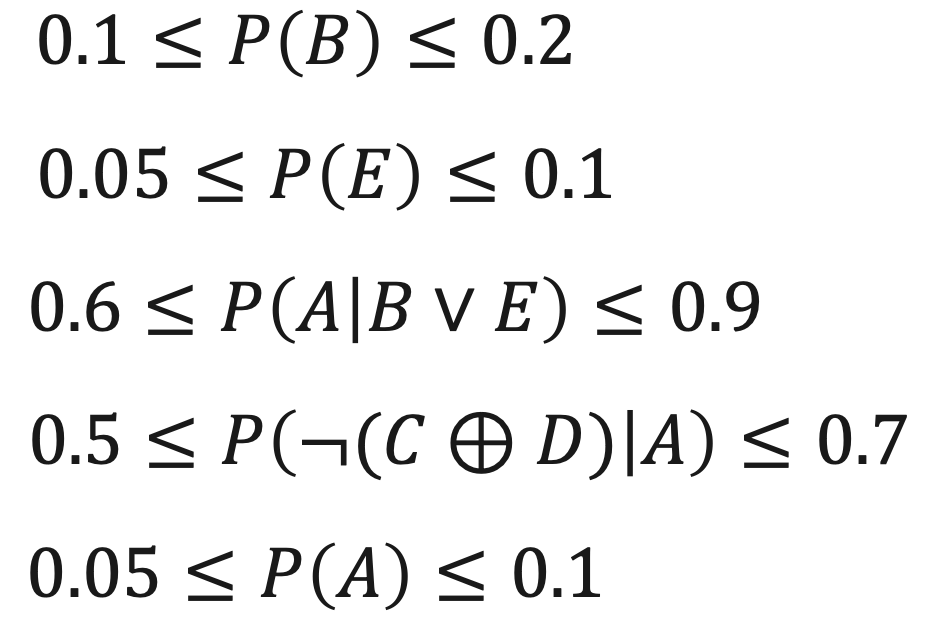
\includegraphics[width=\textwidth]{figs/fig-lcn2.png}
    \caption{LCN constraints}
    \label{fig:constr}
  \end{subfigure}
  \quad
  \begin{subfigure}{0.3\textwidth}
    \centering
    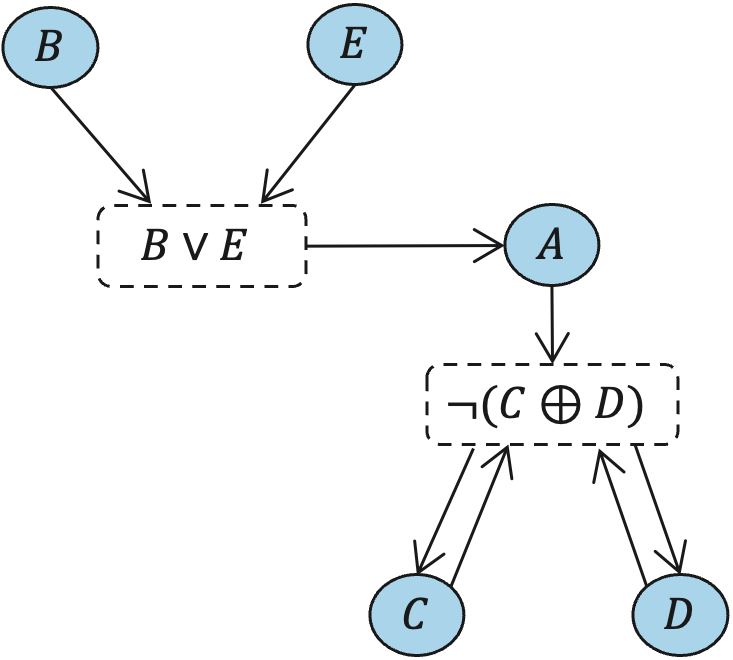
\includegraphics[width=\textwidth]{figs/fig-lcn2-pg.png}
    \caption{LCN primal graph}
    \label{fig:primal}
  \end{subfigure}
  \quad\quad
  \begin{subfigure}{0.3\textwidth}
    \centering
    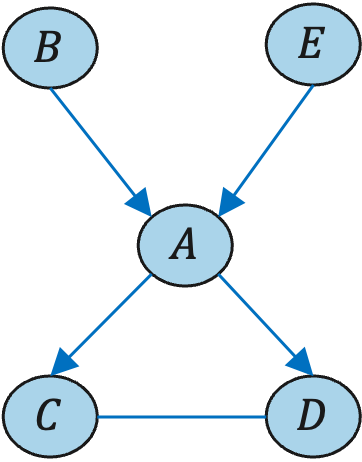
\includegraphics[scale=0.8]{figs/fig-lcn2-st.png}
    \caption{LCN structure (chain graph)}
    \label{fig:struct}
  \end{subfigure}
  \caption{A simple LCN instance with its primal graph and corresponding structure.}
  \label{fig:alarm}
\end{figure}

\begin{example}
    Figure \ref{fig:alarm} shows a simple LCN with 5 propositions and 5 constraints. The corresponding primal graph and structure are given in Figures \ref{fig:primal} and \ref{fig:struct}, respectively. The LMC implies that: $B$ and $E$ are marginally independent, $C$ is conditionally independent of $B$ and $E$ given $C$'s parents $\{A, D\}$, and $D$ is conditionally independent of $B$ and $E$ given $\{A,C\}$, respectively.    
\end{example}

\subsection{Chain Graphs and Factorization}
Let $\bX=\{X_1,\ldots,X_n\}$ be a set of random variables, and let $G=(\cN,E)$ be a graph whose nodes $\cN$ are in one-to-one correspondence with the variables in $\bX$. We denote a configuration of $\bX$ by $\bx$.


\begin{definition}[chain graph]
Let $G=(\cN,E)$ be a mixed graph with $E=E_{\to}\cup E_{-}$, where $E_{\to}$ is a set of directed edges and $E_{-}$ is a set of undirected edges. The graph $G$ is a \emph{chain graph} if there exists a partition
$\cN = \cT_1 \,\dot\cup\, \cT_2 \,\dot\cup\, \cdots \,\dot\cup\, \cT_m$ such that: (i) for each $i$, the subgraph induced by $\cT_i$ contains only undirected edges; (ii) for $i\neq j$, every edge between $\cT_i$ and $\cT_j$ is directed, and all such edges have the same orientation; (iii) the directed graph obtained by contracting each chain component $\cT_i$ into a single node is acyclic. The sets $\cT_1,\ldots,\cT_m$ are called the \emph{chain components} of $G$.
\end{definition}

If there is a directed edge from $A$ to $B$ in $G$ then $A$ is a \emph{parent} of $B$ and $B$ is a \emph{child} of $A$. The parents of $A$ are denoted $\mathbf{pa}(A)$. If there is an undirected edge $A-B$ then both nodes are said to be \emph{neighbors}. The neighbors of $A$ are denoted by $\mathbf{ne}(A)$. The \emph{boundary} of a node $A$, denoted $\mathbf{bd}(A)$, is the set $\mathbf{pa}(A)\cup \mathbf{ne}(A)$. The boundary of a set $\cB$ of nodes is $\mathbf{bd}(\cB) = \bigcup_{A\in \cB} \mathbf{bd}(A) \setminus \cB$. The Local Markov Condition (LMC(C)) for chain graphs is defined as follows:

\begin{definition}[LMC(C)]\label{def:lmc-cg}
    Let $G$ be a chain graph. A node $A\in G$ is independent, given its boundary $\mathbf{bd}(A)$, of all nodes that are not $A$ itself nor descendants of $A$ nor boundary nodes of $A$.
\end{definition}

Given a chain graph $G$ over variables $\bX$, it can be shown that for strictly positive probabilities the local and global Markov conditions are equivalent \citep{cowell99,cozman23a}. The implication is that the joint distribution $P(\bX)$ factorizes according to $G$ as:
\begin{equation}\label{eq:factorization}
P(\bX=\bx) = \prod_{i=1}^m P(\cT_i=\bx_{\cT_i}\mid\mathbf{pa}(\cT_i)=\bx_{\mathbf{pa}(\cT_i)}),
\end{equation}
where the chain components are ordered so that directed edges can only point from earlier to later components, $\mathbf{pa}(\cT_i)$ denotes the set of nodes outside $\cT_i$ with directed edges into $\cT_i$, and $\bx_{\cT_i}$ and $\bx_{\mathbf{pa}(\cT_i)}$ are the projections of $\bx$ onto the corresponding variables. 
Consequently, for an LCN whose structure is a chain graph, the local Markov condition for LCNs (Definition~\ref{def:lmc-lcn}) coincides with Definition~\ref{def:lmc-cg} and every distribution in $\DLCN$ admits the factorization in \eqref{eq:factorization} \citep{cozman23a}.


%% ================================================================
\section{From LCNs to Credal Networks}
\label{sec-lcn-to-credal}
%% ================================================================

In this section, we establish the connection between LCNs and credal networks by exploiting the chain-graph factorization induced by the structure of an LCN. Specifically, we focus on LCNs whose underlying structure is a chain graph, referred to as \emph{chain-graph LCNs}, and show how to reduce inference in LCNs to inference in a credal network. We first provide a brief overview of credal networks \citep{cozman2000credal}. 

% In this section, we leverage the chain-graph factorization of an LCN to reduce exact inference in LCNs to inference in a credal network \citep{cozman2000credal}. We therefore focus on LCNs whose underlying structure is a chain graph, referred to as \emph{chain-graph LCNs}. We first provide a brief overview of credal networks.

\subsection{Credal Networks}
A \emph{credal network} (CN) \citep{cozman2000credal} is defined by a tuple $\langle \bX, \bD, \bK, G \rangle$, where $\bX=\{X_1, \ldots, X_n\}$ is a set of discrete variables with finite domains $\bD=\{D_1, \ldots, D_n\}$, $G$ is a directed acyclic graph (DAG) over $\bX$ as nodes, and $\bK=\{K(X_i\mid \mathbf{pa}(X_i)=\pi_{ik})\}$ is a set of separately specified conditional credal sets for each variable $X_i$ and each $k$-th configuration $\pi_{ik}$ of its parents $\mathbf{pa}(X_i)$ in $G$. A credal set is a set of probability distributions \citep{levi80book} and we consider credal sets that are closed and convex with a finite number of vertices (e.g., probability intervals). The \emph{strong extension} $\DSE$ of a credal network is the \emph{convex hull} (denoted CH) of all joint distributions that satisfy the following Markov property: every variable is strongly independent of its non-descendants conditional on its parents \citep{cozman2000credal,maua2020ijar}.
\begin{equation}\label{eq:se}
    \DSE=\textrm{CH}\{P(\bX)~:~ P(\bX)=\prod_{i=1}^{n} P(X_i\mid \pi_{ik}),~ P(X_i\mid \pi_{ik}) \textrm{~is a vertex of~} K(X_i\mid \pi_{ik})\}
\end{equation}

%It can be shown that the strong extension $\kr{\bX}$ can be built from the extreme points of the conditional local credal sets denoted by $\textrm{ext}(\kr{X_i|\mathbf{pa}(X_i)=\pi_{ik})}$ \citep{maua2020ijar}. 

\subsection{The Chain Graph Approximation for LCNs}
Given a chain-graph LCN $\mathcal{L}$ over variables $\bX=\{X_1,\ldots,X_n\}$, we approximate $\DLCN$ by the strong extension $\DSE$ of an induced credal network. The construction is based on the chain components $\mathcal{T}_1,\ldots,\mathcal{T}_m$ of the underlying chain graph. We first build a DAG $G'$ whose nodes correspond to these chain components. Each node represents the joint state space of the variables in the corresponding chain component, that is, the Cartesian product of their domains. Thus, a node corresponds to a compound variable whenever its chain component contains multiple variables, and to a single LCN variable otherwise. Let $v$ denote a family in $G'$, consisting of a child node $ch_v$ and its parent set $pa_v$. For each parent configuration $pa_v=\pi$, we define a local credal set $K(ch_v\mid pa_v=\pi)$ (or $K_v$ for short) by computing lower and upper bounds on the conditional probabilities of $ch_v$ given $\pi$. Following the standard LCN encoding of \citet{marinescu2022neurips}, these bounds are obtained by solving a local optimization problem involving only the probabilistic sentences whose variables belong to $ch_v \cup pa_v$. The resulting fractional linear programs (LPs) are solved using the Charnes--Cooper transformation \citep{charnes1962flp}.

\begin{figure}[t]
  \centering
  \begin{subfigure}{0.2\textwidth}
    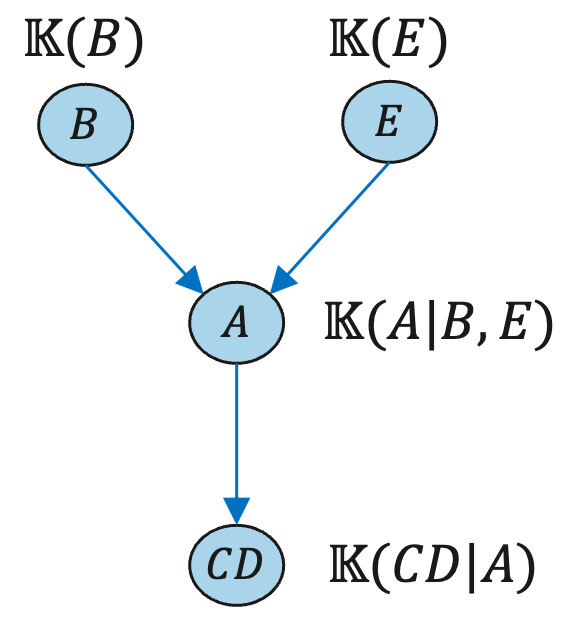
\includegraphics[width=\textwidth]{figs/fig-cn.png}
    \caption{Credal network}
    \label{fig:cn}
  \end{subfigure}
  \quad
  \begin{subfigure}{0.4\textwidth}
    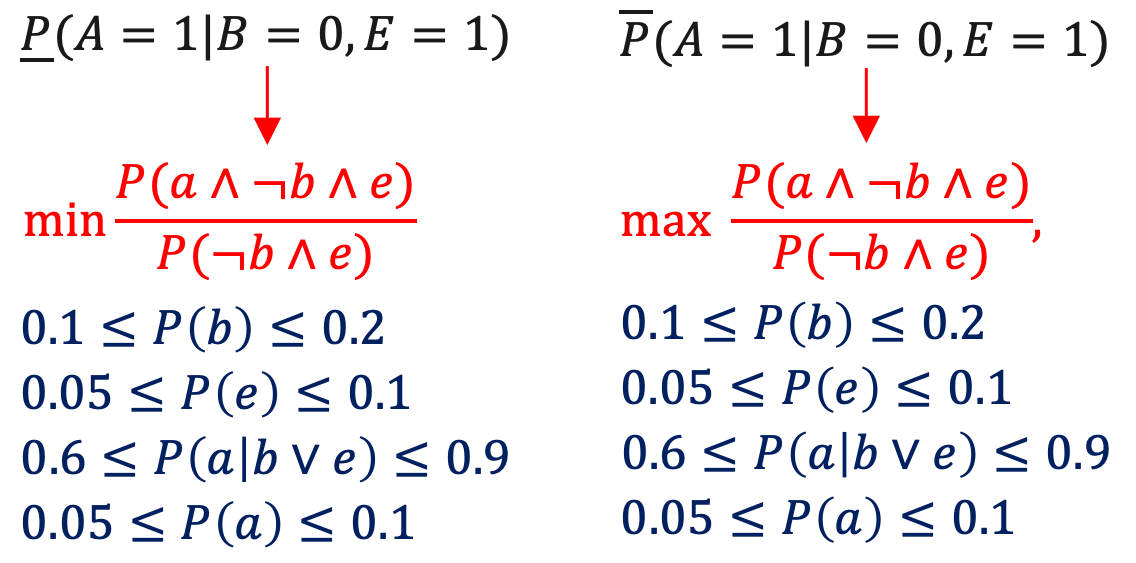
\includegraphics[width=\textwidth]{figs/fig-flp.png}
    \caption{Local fractional LPs}
    \label{fig:flp}
  \end{subfigure}
  \quad
  \begin{subfigure}{0.3\textwidth}
    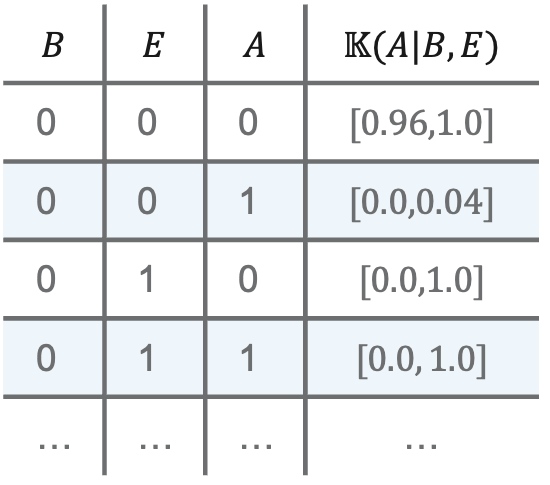
\includegraphics[width=.8\textwidth]{figs/fig-cset2.png}
    \caption{Local credal set}
    \label{fig:cset}
  \end{subfigure}
  \caption{The credal network for the chain-graph factorization of the LCN from Figure \ref{fig:alarm}.}
  \label{fig:factorization}
\end{figure}

\begin{example}
    Figure \ref{fig:cn} shows the credal network induced by the chain-graph factorization of the LCN from Figure \ref{fig:alarm}. Any joint distribution in $\DSE$ factorizes as 
    $P(B)\cdot P(E) \cdot P(A\mid B,E) \cdot P(C,D\mid A)$. In Figure \ref{fig:flp} we outline the fractional LPs for computing lower and upper bounds on $P(A=1\mid B=0,E=1)$, respectively. A partial local credal set $K(A\mid B,E)$ is given in Figure \ref{fig:cset}.
\end{example}

Given a reference credal set $\mathcal{R}$ with true query bounds $[\underline{q}^\star,\overline{q}^\star]$, an estimated interval is \emph{exact} when it equals the true bounds, an \emph{outer bound} when it encloses them, and an \emph{inner bound} when it is enclosed by them. Intervals that satisfy neither property are termed \emph{unreliable}. We can show that:

\begin{proposition}[inclusion]\label{prop:inclusion}
  For any chain-graph LCN, $\DLCN \subseteq \DSE$. Consequently, any inference algorithm that is \emph{exact} or \emph{outer} for $\DSE$ computes valid \emph{outer bounds} for $\DLCN$.
\end{proposition}

\subsection{Family-realizable Sentences}
\label{sec:realizable}

The proposed approximation introduces two looseness gaps. First, each $K_v$ is computed per family in isolation, so it may admit conditionals that no global $p\in \DLCN$ realizes -- it ignores sentences on other families and the cross-family LMC equalities. Formally $K^{\mathrm{true}}_v \subseteq K_v$, sometimes strictly. Second, even with $K_v = K_v^{\mathrm{true}}$, the free product of \eqref{eq:se} lets each family pick its row independently, which can violate a sentence whose scope spans several families. We therefore introduce a class of LCN sentences, called \emph{family-realizable sentences}, and identify conditions when $\DSE = \DLCN$.


\begin{definition}[family-realizable sentence]\label{def:realizable}
Let $\mathcal L$ be a chain-graph LCN with families $\{(\ch_v,\pa_v)\}$, and let $s$ be a sentence
with functional $g_s$. Say $s$ is \emph{family-realizable in family $v$} if $\atoms(s)\subseteq
\ch_v\cup\pa_v$ and the value $g_s(p)$ is determined by the conditional table
$P(\ch_v\mid\pa_v)$ \emph{alone} --- i.e.\ for any two joints $p,p'$ that induce the same conditional
table at $v$, $g_s(p)=g_s(p')$, whatever the parents' marginals $P(\pa_v)$ and $P'(\pa_v)$ may be.
Concretely, $s$ is family-realizable in $v$ if and only if it has one of the two forms:
\begin{enumerate}
  \item[\textup{(R1)}] \emph{Type-1 on a root block:} $s$ is $\ell\le P(\varphi)\le u$ with
    $\atoms(\varphi)\subseteq\ch_v$ and $\pa_v=\varnothing$. Then $P(\varphi)$ is a function of
    $P(\ch_v)$, which \emph{is} the family's table.
  \item[\textup{(R2)}] \emph{Type-2 pinning one full parent configuration:} $s$ is
    $\ell\le P(\varphi\mid\psi)\le u$ with $\atoms(\varphi)\subseteq\ch_v$,
    $\atoms(\psi)\subseteq\pa_v$, and $\psi$ satisfied by \emph{exactly one} assignment $\pi^\star$
    of $\pa_v$. Then $P(\varphi\mid\psi)=P(\varphi\mid\pa_v{=}\pi^\star)$ is a single row of the
    table.
\end{enumerate}

A sentence is \emph{non-realizable} if it is family-realizable in no family. The LCN is \emph{fully
realizable} if every sentence is family-realizable in some family\footnote{Note that a sentence can be attached to several families while being realizable in only one of them.}.
\end{definition}

\begin{proposition}[sufficiency]\label{prop:suff}
Let $\mathcal L$ be a chain-graph LCN with families $\{(ch_v, pa_v)\}$ and local credal sets built by the chain-graph approximation. Suppose (i) for every family $v$ and parent configuration $\pi$, $K_{v,\pi}=K_{v,\pi}^{\mathrm{true}}$, the projection of $\DLCN$ onto that row; and (ii) every sentence of $\mathcal L$ is family-realizable in some family (Definition~\ref{def:realizable}). Then $\DSE=\DLCN$.
\end{proposition}

We next present three algorithms that compute exact, outer and inner bounds for $\DSE$, respectively.

\subsection{Credal Variable Elimination}
\label{sec-cve}

Credal Variable Elimination (CVE) extends Variable Elimination (VE) for Bayesian networks \citep{dechter-book} to credal networks by propagating  finite sets of non‑negative functions called \emph{potentials} instead of functions \citep{maua2020ijar}.

\begin{definition}[potential]
A \emph{potential} $\phi(\bY)$ over variables $\bY$ is a finite set of non-negative real-valued functions $\{f_1, f_2, \dots, f_m\}$ on the joint domain of $\bY$. The \emph{product} (or combination) of two potentials is defined by $\phi \cdot \psi = \{f \cdot g : f \in \phi, \; g \in \psi\}$, where $(f \cdot g)(\by, \bz) = f(\by) \cdot g(\bz)$ over the joint domain $\bY \cup \bZ$. The \emph{sum-marginal} is defined by $\sum_{X} \phi(\bY) = \{ \sum_{x} f(\by) : f \in \phi \}$, producing functions over $\bY \setminus \{X\}$. A \emph{pruning} operation is defined by $prune(\phi) = \{f \in \phi : \nexists\, g \in \phi \setminus \{f\} \text{ s.t.\ } g(\by) \geq f(\by)\; \forall\, \by\}$. 
\end{definition}

Given a query variable $Z$, an elimination order $\mathbf{o}$ such that $Z$ appears last and initial potentials obtained from the extreme points of the conditional credal sets, each potential is assigned to the bucket of the first variable in its scope. The algorithm then processes each bucket, from first to last in the elimination ordering $o$ but excluding $Z$, by multiplying all potentials in the current bucket and eliminating the bucket's variable by summation, resulting in a new potential which is first pruned by its non-maximal elements and then placed in a subsequent bucket, depending on its scope. Processing the last bucket by first multiplying all its potentials, normalizing and taking component-wise minima and maxima yields lower and upper bounds for $Z$ (see Appendix for more details and examples).

Since the intermediate potentials generated by CVE can grow exponentially, we can approximate the potentials by fixing their cardinality to a relatively small number $B$ \citep{maua2020ijar,marinescu2026iclr}. Specifically, we group the elements of $\phi(\bY)$ into $B$ clusters based on minimizing the Manhattan distance to each cluster's centroid (i.e., minimize $\sum_{i=1}^{m} |p_i - r_i|$, where $p_i$ and $r_i$ are the $i$-th components of $p$ and $r$, respectively). Then, for each cluster we replace its components with their mean values. This yields an approximation method denoted by CVE$_{cm}$.

\begin{theorem}[complexity]
    The time and space complexity of CVE is $O(m \cdot C \cdot d^{w^*})$ where $m$ is the number of variables, $d$ bounds the domain size, $w^*$ is the treewidth, and $C$ is the maximum potential cardinality (which can be exponential). With potential approximation, $C$ is bounded by $B$.
\end{theorem}

\begin{theorem}[exactness]
Let $\cL$ be a family-realizable chain-graph LCN. Then CVE computes \emph{exact bounds} with respect to $\DLCN$.
\end{theorem}

% Since some $Y_j$ are compound variables, posterior lower and upper bounds for the corresponding singleton variables $X_{jk}$ can be obtained efficiently by solving a small linear program over the compound marginal polytope \cite{cozman2000credal,maua2020ijar} (see also the Appendix for more details).

\subsection{Interval Belief Propagation}
\label{sec-ibp}

Given a credal network compiled to a \emph{factor graph} \citep{koller2009probabilistic} whose factor nodes $\{f_i\}$ store the finite sets of extreme points $\mathrm{ext}\,K(X_i \mid \pi)$ (one per parent configuration $\pi$ of the associated variable $X_i$), plus evidence $\mathbf{Y} = \mathbf{y}$, our second approach called Interval Belief Propagation (IBP) computes bounds $[\underline{P}(X_i{=}x \mid \mathbf{y}),\, \overline{P}(X_i{=}x \mid \mathbf{y})]$ for every non-evidence variable $X_i$ and every state $x \in D_{X_i}$. Unlike previous algorithms like L2U \citep{l2u} and GL2U \citep{antonucci2010} which are restricted to binary variables, IBP natively handles multi-valued variables.

Each directed edge of the factor graph carries an interval-vector message
$\mu_{v \to f} = (\mathbf{l}_{v \to f}, \mathbf{u}_{v \to f}) \in
[0,1]^{|D_v|} \times [0,1]^{|D_v|}$ (and symmetrically $\mu_{f \to v}$) with
$\mathbf{l} \le \mathbf{u}$ componentwise. All messages are initialized to the
vacuous interval $(\mathbf{0}, \mathbf{1})$. For every evidence assignment
$Y_j = y_j$, the outgoing variable-to-factor messages from $Y_j$ are clamped to
the one-hot indicator
$\mu_{Y_j \to f} \gets (\delta_{y_j}, \delta_{y_j})$ and held fixed throughout.

At every iteration, two sweeps are performed. \emph{Variable-to-factor} messages
(skipped for evidence variables) tighten by intersecting the other incoming
bounds:
\begin{equation}\label{eq:compact-vtof}
  \mathbf{l}_{v \to f} \;=\; \max_{f' \in \mathcal{N}(v) \setminus \{f\}}
                              \mathbf{l}_{f' \to v},
  \qquad
  \mathbf{u}_{v \to f} \;=\; \min_{f' \in \mathcal{N}(v) \setminus \{f\}}
                              \mathbf{u}_{f' \to v}, \qquad v \notin \mathbf{Y}
\end{equation}
(component-wise, over all neighbor factors $\mathcal{N}(v)$ other than $f$). \emph{Factor-to-variable}
messages extremize the target's normalized marginal over two discrete choice
sets:
\begin{equation}\label{eq:compact-ftov}
  \mathbf{l}_{f_i \to v}(x) \;=\; \min_{(\mathbf{vc},\,\mathbf{cc})}
    \tilde{p}_{\mathbf{vc},\mathbf{cc}}(x),
  \qquad
  \mathbf{u}_{f_i \to v}(x) \;=\; \max_{(\mathbf{vc},\,\mathbf{cc})}
    \tilde{p}_{\mathbf{vc},\mathbf{cc}}(x),
\end{equation}
where a \emph{vertex combination} $\mathbf{vc}$ picks one extreme point
$P_{\mathbf{vc}}(X_i \mid \pi) \in \mathrm{ext}\,K(X_i \mid \pi)$ for every
parent configuration $\pi$, a \emph{corner-point combination} $\mathbf{cc}$
picks $\mathbf{q}_w \in \{\mathbf{l}_{w \to f_i}, \mathbf{u}_{w \to f_i}\}$ for
each other-variable $w \in \mathrm{scope}(f_i) \setminus \{v\}$, and
$\tilde{p}_{\mathbf{vc},\mathbf{cc}}(x) = m_{\mathbf{vc},\mathbf{cc}}(x) /
\sum_{x'} m_{\mathbf{vc},\mathbf{cc}}(x')$ with $m_{\mathbf{vc},\mathbf{cc}}$
the unnormalized marginal (see details and examples in Appendix). The two sweeps are repeated until the maximum component-wise change across all
messages falls below a tolerance $\tau$, or a cap of $T$ iterations is reached.
The final conditional marginal bounds for every variable are obtained by
intersecting all factor-to-variable messages incident on it:
\begin{equation}\label{eq:compact-extract}
  \underline{P}(X_i{=}x \mid \mathbf{y}) = \max_{f \in \mathcal{N}(X_i)}
    \mathbf{l}_{f \to X_i}(x),
  \qquad
  \overline{P}(X_i{=}x \mid \mathbf{y}) = \min_{f \in \mathcal{N}(X_i)}
    \mathbf{u}_{f \to X_i}(x).
\end{equation}


\begin{theorem}[complexity]
    The complexity per iteration of IBP is $O(N_f \cdot V_{\max} \cdot 2^{S_{\max}} \cdot k^{S_{\max}})$, where $N_f$ is the number of factors, $V_{\max}$ the maximum vertex combinations per factor, $S_{\max}$ the maximum scope size, and $k$ the maximum domain size.
\end{theorem}

\begin{theorem}[exactness]
    Let $\mathcal{L}$ be a family-realizable chain-graph LCN. If $\mathcal{L}$'s structure is singly connected (i.e., a tree), then IBP computes \emph{exact bounds} with respect to $\DLCN$.
\end{theorem}

\subsection{Coordinate Descent with Variable Elimination}
\label{sec-cdve}
Our third approach called Coordinate Descent with Variable Elimination (CDVE) extends the ApproxLP method \citep{antonucci2015approxlp} that reformulates credal marginal inference as a multilinear program and solves it via coordinate descent. In our case, for every non-evidence variable $Z$, CDVE runs coordinate descent twice --- once with sense $\min$ and once with sense $\max$. Each run starts by initializing all $P(X_i \mid \pi_i)$ at the centroid of their respective credal sets and computing by exact Variable Elimination (VE) $p^* = \mathrm{VE}(\{P\}, Z)$, the full posterior vector on $D_Z$ under these fixed distributions. A \emph{sweep} then visits every $(X_i, \pi_i)$: for each vertex $v \in \mathrm{ext}\,K(X_i \mid \pi_i)$, it temporarily sets $P(X_i \mid \pi_i) \gets v$, re-evaluates $\mathrm{VE}$, and accepts $v$ (strictly, else rejects) if the target component $p^*(z)$ moves in the sense's direction. Sweeps repeat until one produces no improvement or the cap $T$ is reached. Because each $\mathrm{VE}$ call returns a full vector, the two runs together yield componentwise bounds $[\underline{p}(z), \overline{p}(z)]$ for every state $z \in D_Z$ simultaneously. Evidence variables (if any) are skipped by a point-mass shortcut. The output is \emph{inner bounds} for $\DSE$ --- coordinate descent explores only a subset of feasible vertex combinations, so the returned interval is contained in the true interval. 

\begin{theorem}[complexity]
    The time and space complexity of CDVE is $O(T \cdot V_{\text{total}} \cdot n \cdot k^{w^*})$ and $O(n\cdot k^{w^*})$, where $V_{\text{total}}$ is the total number of extreme points across all credal sets, $k$ bounds the domain size, and $w^*$ is the induced width.    
\end{theorem}


%% ================================================================
\section{Exact LCN Inference at Treewidth Cost}
\label{sec-cjt}
%% ================================================================

Recall that exact inference in LCNs amounts to computing the lower and upper probabilities $\lo P(a)=\min_{p \in \DLCN}P(a)$ and $\hi P(a)=\max_{p \in \DLCN}P(a)$, respectively. Direct optimization over $\DLCN$ requires a nonlinear program with $2^n$ variables \citep{marinescu2022neurips}. Alternatively, compiling the LCN into a credal network and performing inference as described in Section~\ref{sec-lcn-to-credal} is computationally cheaper, but in general yields bounds over the strictly larger strong extension $\DSE$.

To address these limitations, we introduce Credal Junction Tree (CJT), a novel algorithm for exact inference in LCNs. CJT preserves the exactness of the nonlinear optimization approach of \citet{marinescu2022neurips} while requiring a nonlinear program that is exponentially smaller. The key idea is to exploit a junction-tree decomposition of the credal network induced by the chain-graph factorization. Specifically, CJT first moralizes and triangulates the underlying chain graph, producing a chordal graph $G^\ast$. It then constructs a junction tree $T$ whose clusters $\mathcal{C}$ satisfy the running-intersection property \citep{dechter-book}. For each cluster $C\in\mathcal{C}$, the algorithm introduces a local marginal variable vector $q_C\in\Delta(2^{|C|})$ representing a distribution over the variables in $C$. Exact inference is then reduced to the following optimization problem (see the Appendix for more details and examples):
\[
\begin{aligned}
\min/\max\quad & \readoff_a(q)\\
\text{s.t.}\quad
&\textstyle\sum_i q_{C,i}=1,\ q_{C,i}\ge0 && \forall C\in\mathcal C,\\
&q_C\restr S=q_D\restr S && \forall (C,D)\in T,\ S=C\cap D,\\
&\ell\langle A_{\psi},q_{C_h}\rangle\le\langle A_{\varphi\wedge\psi},q_{C_h}\rangle
   \le u\langle A_{\psi},q_{C_h}\rangle && \forall\text{ sentence hosted on }C_h,\\
&\langle A_a,q\rangle\langle A_b,q\rangle=\langle A_c,q\rangle\langle A_d,q\rangle
   && \forall\text{ LMC assertion hosted,}
\end{aligned}
\]
where $A_\varphi$ is the $0/1$ indicator vector of $\varphi$ over the host cluster's
states, a constraint is \emph{hosted} on any cluster containing its scope, $\langle A_{\varphi},q \rangle$ is the dot-product of two vectors, and $\readoff_a$ reads $P(a)$ (or $P(a\mid \textbf{e})$, via one auxiliary variable) off a
cluster containing $a$ and the evidence. For every pair of adjacent clusters $C$ and $D$, the marginals induced on their separator $S$, denoted by $q_C\restr S$ and $q_D\restr S$, are required to coincide, ensuring global consistency. An LMC assertion whose conditioning set
separates its two sides in $G^\ast$ is \emph{separator-entailed} and is omitted:
the junction tree's topology already enforces it. The program is nonconvex through the
bilinear LMC assertions and is solved globally.

\begin{theorem}[exactness]\label{thm:cjt}
Let $\cL$ be a chain-graph LCN and $T$ a junction tree of its chordal graph $G^\ast$. Assume that \textup{(H1)} $T$ satisfies the running-intersection property; \textup{(H2)} every probabilistic sentence is hosted by some cluster of $T$; \textup{(H3)} every LMC assertion is either hosted by a cluster or
separator-entailed in $G^\ast$; \textup{(H4)} the query and evidence variables are contained in a common cluster. Then CJT computes \emph{exact} lower and upper probabilities over $\DLCN$.
\end{theorem}

The formulation needs $\sum_C2^{|C|}{=}O(n2^{w+1})$ variables and $O(n2^w)$ separator-consistency constraints making its complexity exponential in the treewidth $w$ rather than in the number of variables $n$. 


%% ================================================================
\section{Experiments}
\label{sec-experiments}
%% ================================================================

In this section, we evaluate the proposed marginal inference schemes on several classes of LCNs, comparing them with the exact method of \citet{marinescu2022neurips} and the approximate ARIEL algorithm \citep{marinescu2023lcn}. All algorithms are implemented in Python 3.12 and use \texttt{ipopt} 3.14 \citep{ipopt} for the nonlinear programs. Every run has a limit of $3600$ seconds and $30$\,GB of memory; a dash in a table means the algorithm did not finish inside that budget.

\begin{figure}[!t]
    \centering
    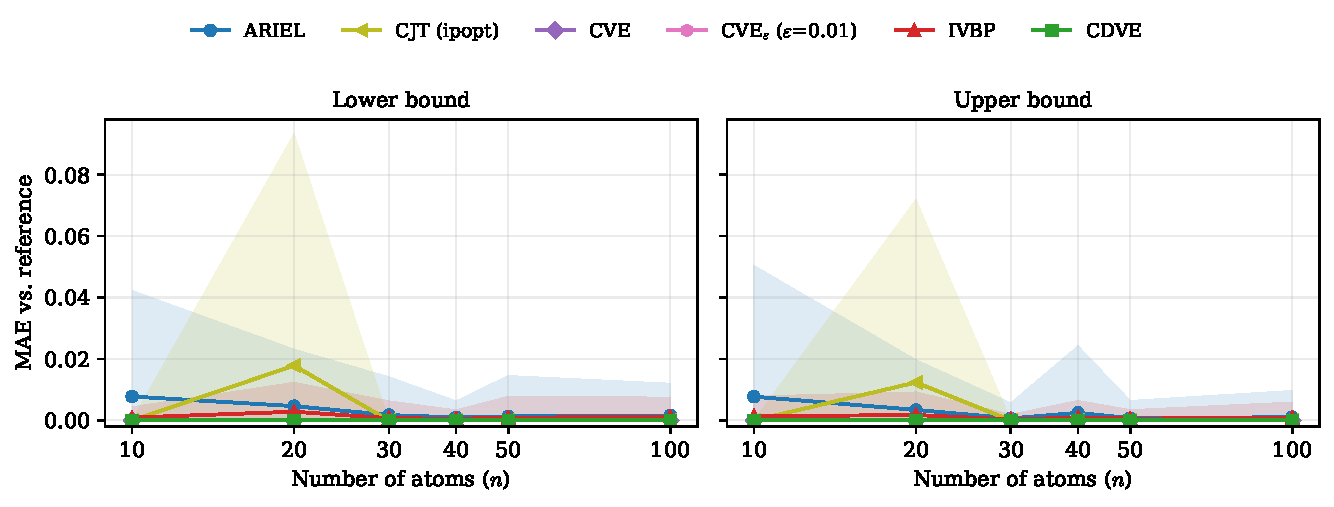
\includegraphics[height=3.6cm]{figs/dag_large_fr_mae.pdf}
    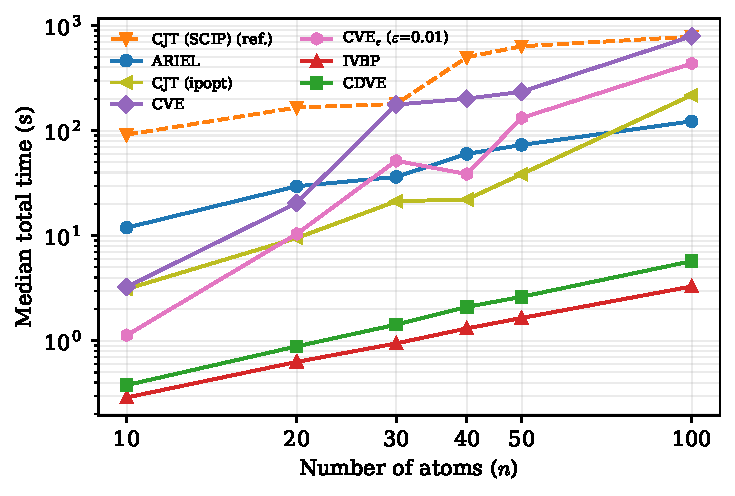
\includegraphics[height=3.6cm]{figs/dag_large_fr_runtime.pdf}
    \caption{Large random \texttt{dag} LCNs: (left) MAEs against
    the CJT reference, with bands giving one standard deviation over 10 instances per size -- curves stopping where the budget was exceeded; (right) total time in seconds.}
    \label{fig:random}
\end{figure}

\begin{table}[!t]
\centering
\footnotesize
\begin{tabular}{llrrr}
\toprule
Instance & Algorithm & MAE$_{l}$ & MAE$_{u}$ & Time (s) \\
\midrule
Alarm ($n{=}10$), CJT ref 0.72s & ARIEL & 0.000 & 0.000 & 3.92 \\
 & IBP & 0.101 & 0.015 & 0.13 \\
 & CDVE & 0.101 & 0.015 & 0.69 \\
 & CVE$_{cm}$ & 0.087 & 0.067 & 0.24 \\
\hline
Credit ($n{=}11$), CJT ref 1.15s & ARIEL & 0.050 & 0.000 & 3.18 \\
 & IBP & 0.257 & 0.000 & 0.24 \\
 & CDVE & 0.257 & 0.000 & 0.69 \\
 & CVE$_{cm}$ & 0.108 & 0.165 & 1.73 \\
\hline
Hepatitis ($n{=}10$), CJT ref 0.56s & ARIEL & 0.008 & 0.008 & 3.91 \\
 & IBP & 0.069 & 0.080 &  0.75 \\
 & CDVE & 0.070 & 0.085 & 1.15 \\
 & CVE$_{cm}$ & 0.114 & 0.184 & 16.53 \\
\hline
MScaling ($n{=}12$), CJT ref 0.66s & ARIEL & 0.028 & 0.000 & 8.13 \\
 & IBP & 0.129 & 0.493 &  0.35 \\
 & CDVE & 0.129 & 0.501 &  1.23 \\
 & CVE$_{cm}$ & 0.079 & 0.227 & 0.57 \\
\hline
BScaling ($n{=}32$), CJT ref 2.42s & ARIEL & 0.000 & 0.000 &  19.80 \\
 & IBP & 0.115 & 0.225 &  0.69 \\
 & CDVE & 0.115 & 0.225 &  20.55 \\
 & CVE$_{cm}$ & 0.064 & 0.072 &  9.18 \\
\hline
PScaling ($n{=}40$), CJT ref 3.27s & ARIEL & 0.000 & 0.000 & 34.72 \\
 & IBP & 0.129 & 0.263 & 0.91 \\
 & CDVE & 0.129 & 0.263 & 51.25 \\
 & CVE$_{cm}$ & 0.070 & 0.057 &  658.84 \\
\bottomrule
\end{tabular}
\caption{Realistic LCNs: three instances derived from real Bayesian networks
(top) and three Supreme Court chain-graph instances (bottom), all against the
CJT reference. Time is total time including the credal-network build; the reference's own time on each instance is given with the
instance name.}
\label{tab:real}
\end{table}

% Recall that family-realizability means each sentence constrains a single family's conditional table alone and the credal-network relaxation
% is exact \emph{iff} the primal graph is singly connected \emph{and} every sentence
% is realizable. So \texttt{tree} and \texttt{polytree} probe the tight regime, while
% \texttt{ktree} and \texttt{dag} are realizable but loopy --- any two-parent collider
% moralizes into a cycle --- and there the methods give outer bounds only.

\textbf{Benchmarks.~}
We consider two types of LCN instances. \emph{Random LCNs} come in four
topologies, each generated so that every sentence is \emph{family-realizable}:
\texttt{tree}, \texttt{polytree}, \texttt{ktree} ($k{=}3$) and \texttt{dag}
(moralized treewidth $\le 3$, at most two parents per atom). Each topology is
generated at two scales, \emph{small} ($n \in \{5,\dots,10\}$) and \emph{large}
($n \in \{10,20,30,40,50,100\}$), with $10$ instances per size, giving
$8 \times 60 = 480$ instances. Sentence bounds are drawn as
$[\max(0.01, v{-}\varepsilon), \min(1, v{+}\varepsilon)]$ with $v \sim U(0,1)$
and $\varepsilon = 0.3$; formulas span at most three atoms; two extra marginals
per instance are placed on root atoms only; the seed is $42$. Every instance is accepted only after a product-distribution
consistency witness is found,
so all $480$ are consistent by construction. \emph{Realistic LCNs} are of two kinds: ten
instances derived from real Bayesian networks \citep{bn-repo} ($n = 4$--$11$,
$6$--$24$ sentences), and sixteen instances from the causal chain graphs of the
US Supreme Court analysis of \citet{ogburn2020causal}. The latter stress two
different axes: the \texttt{scaling} instances are large and sparse
($n = 6$--$40$, $11$--$79$ sentences), whereas the \texttt{supreme\_court}
instances are small but extremely dense ($n{=}10$ with $345$--$1009$ sentences).

\textbf{Algorithms, reference and metrics.~}
We compare four approximate algorithms: ARIEL \citep{marinescu2023lcn},
which operates directly on the LCN factor graph ($10$ iterations) and needs no
credal-network build; IBP, interval belief propagation on the credal
network ($100$ iterations); CDVE, coordinate descent over extreme points
($50$ iterations), which by construction returns \emph{inner} bounds; and
CVE$_{cm}$, Credal Variable Elimination with its intermediate
potentials clustered to at most $10$ functions using the mean representative.
Plain CVE (exact over the strong extension, no clustering) is included
where it terminates. All credal-network methods share the same build:
the chain-graph factorization, no scope merging, and per-family local credal
sets solved as linear programs. As the reference we use CJT, the junction-tree NLP formulation
(using the \texttt{ipopt} backend): it is the
tightest engine tractable at every size here, whereas exact inference of \citet{marinescu2022neurips} over the
$2^n$ joint solves only $15/60$ of \texttt{tree\_small} and none of the Supreme
Court instances. We report the mean absolute error of the lower and upper marginal bounds against the reference,
$\mathrm{MAE}_{l} = \frac{1}{n}\sum_i |\underline{P}^{*}(x_i) -
\underline{P}(x_i)|$ and $\mathrm{MAE}_{u}$ analogously, and wall-clock time in seconds including the credal-network
build. Note that CJT's build is not comparable to the others': it needs only
the chain-graph structure and skips the vertex enumeration entirely. 
Recall that family realizability requires each sentence to constrain a single family conditional distribution. Thus, for singly connected family-realizable LCNs (e.g., \texttt{tree} and \texttt{polytree}), both IBP and CVE are exact. For family-realizable but loopy LCNs (e.g., \texttt{ktree} and \texttt{dag}), where moralization creates cycles, only CVE is guaranteed to be exact.

\textbf{Random LCNs.~}
Figure~\ref{fig:random} shows the loopy \texttt{dag} LCNs at the large scale,
with shaded bands giving one standard deviation over the ten instances per size (full results on all LCNs are included in the Appendix). Three findings
hold across all four topologies. First, IBP dominates: its error against the reference
is at or below $4 \times 10^{-3}$ on every scale (small, large) and size --- indistinguishable
from CJT on \texttt{tree} and \texttt{polytree}, as the exactness
characterization predicts --- while being the fastest method everywhere, by one
to three orders of magnitude at $n{=}100$. Second, CDVE matches that
accuracy but not that cost: its mean error stays in the $10^{-3}$ range, yet its
runtime grows from under a second on the small instances to $273$--$614$ seconds
on the large ones, making it slower than ARIEL at $n{=}100$. ARIEL is likewise
accurate (exactly zero error on \texttt{tree} and \texttt{polytree}) but pays
$25$--$35$ seconds at scale. Third, approximating the potentials by clustering buys speed at a real cost
in quality: CVE$_{cm}$ runs in a fraction of a second on the small instances but
its error grows with $n$, from $0.08$--$0.11$ on the small instances to
$0.31$--$0.35$ on the large ones. Plain CVE is the
scalability bottleneck: it is essentially exact where it runs but costs
$226$--$1141$ seconds, times out on all of \texttt{ktree\_small} and
\texttt{polytree\_large}, and is intractable on the large loopy LCNs.

\textbf{Realistic LCNs.~}
Table~\ref{tab:real} reports six representative instances. These instances are chain-graph LCNs but they are not family-realizable and therefore Proposition \ref{prop:suff} does not hold. The ordering is
different here: ARIEL is clearly the tightest method, at or near zero error on
four of the six instances, because it reasons on the original LCN rather than on
its credal-network relaxation. IBP and CDVE agree closely and produce widths $1.4$--$7.7\times$ the reference ---
genuine but loose outer bounds, the gap being the cost of the relaxation rather
than a defect of the message passing. On running time the picture is again favourable to IBP, which is the
fastest method on every instance and the only one that stays under a second at
$n{=}40$, where CDVE needs $51$ seconds and CVE$_{cm}$ $659$. 



%% ================================================================
\section{Related Work}
\label{sec-related}
%% ================================================================

Credal networks (CNs) \citep{cozman2000credal} generalize Bayesian networks by replacing precise conditional probabilities with credal sets. Despite the computational hardness of exact inference \citep{maua2020ijar}, the area has produced a rich algorithmic toolbox, including 2U/L2U~\citep{l2u}, GL2U~\citep{antonucci2010}, and ApproxLP~\citep{antonucci2015approxlp}. In contrast, inference in LCNs remains largely unexplored, with existing methods limited to exact constrained nonlinear optimization~\citep{marinescu2022neurips} and the ARIEL message-passing algorithm~\citep{marinescu2023lcn}; related work has focused on abductive reasoning~\citep{marinescu2024neurips} and the theoretical development of chain-graph factorizations~\citep{cozman23a}. Our work closes this gap by turning the latter into an algorithmic bridge between LCNs and CNs, enabling the first systematic transfer of credal-network inference methods to the LCN setting. More broadly, LCNs are related to probabilistic logic frameworks such as ProbLog~\citep{problog}, DeepProbLog~\citep{manhaeve2018deepproblog}, MLNs~\citep{mln}, and PSL~\citep{bach2017psl}, but are distinguished by their support for imprecise probability assessments and minimal structural assumptions.

%% ================================================================
\section{Conclusion}
\label{sec-conclusion}
%% ================================================================

In this paper, we introduced a credal network perspective on Logical Credal Networks, yielding the first general framework for transferring credal network inference algorithms to the LCN setting. This connection led to a family of exact and approximate inference methods, including CVE, CVE$_{cm}$, IBP, CDVE, and CJT. In particular, CJT achieves exact LCN inference by exploiting a junction-tree decomposition to solve an exponentially smaller nonlinear program than previous exact approaches. Our theoretical and empirical results show that these methods substantially expand the scalability-accuracy trade-off space for LCN inference, thus providing a richer algorithmic toolbox for reasoning under logical and probabilistic uncertainty.

%%%%%%%%%%%%%%%%%%%%%%%%%%%%%%%%%%%%%%%%%%%%%%%%%%%%%%%%%%%%%%%%%%%%%%%%%%%%%
\subsection*{AI use statement}

We used generative AI tools to assist with language editing, grammar correction, and code development. In particular, AI-assisted coding tools were used during the implementation of the proposed algorithms. All AI-generated content was reviewed, verified, and, where applicable, extensively tested by the authors. For example, AI-generated code was manually inspected for correctness and validated through unit and integration testing. The authors take full responsibility for the accuracy, validity, and integrity of all content presented in this paper.


\subsection*{Ethics statement}

%(This section is \textbf{recommended} and does not count toward the page limit.)

This work did not involve human subjects.

\subsection*{Reproducibility statement}

%(This section is \textbf{recommended} and does not count toward the page limit.)

To ensure reproducibility, we have included the Python code and benchmark problem instances in the supplementary material. We will open-source the code and benchmarks if the paper is accepted. 

% \subsubsection*{Author Contributions}
% If you'd like to, you may include  a section for author contributions as is done
% in many journals. This is optional and at the discretion of the authors.

% \subsubsection*{Acknowledgments}
% Use unnumbered third level headings for the acknowledgments. All
% acknowledgments, including those to funding agencies, go at the end of the paper.


\bibliography{ref}
\bibliographystyle{iclr2027_conference}

\appendix

%% ================================================================
\section{Preliminaries}
\label{sec:prelim}
%% ================================================================

A Logical Credal Network specifies imprecise probabilistic knowledge by
bounding the probabilities of propositional formulas: a \emph{sentence} is either
$\ell\le P(\varphi)\le u$ (Type-1) or $\ell\le P(\varphi\mid\psi)\le u$
(Type-2), over propositional formulas $\varphi,\psi$ on binary atoms. Together
with the independence assumptions that the Local Markov Condition derives from
the program's structure, a set of sentences determines a closed set $\DLCN$ of
joint distributions, and the inference task is to compute
$\lo P(a)=\min_{p\in\DLCN}P_p(a)$ and $\hi P(a)=\max_{p\in\DLCN}P_p(a)$ for each
atom $a$.

Two families of inference methods exist. The \emph{direct} exact method of \cite{marinescu2022neurips}
writes one variable per joint state and optimizes over
$\DLCN$ itself; it is exact when its solver certifies global optimality, but its
$2^n$ formulation confines it to small instances. The
\emph{credal-network} family described in this paper (CVE, IBP, CDVE) compiles the LCN into a chain-graph credal network with interval local credal sets, and propagates messages; it scales, but it optimizes over the strong
extension $\DSE\supseteq\DLCN$.

\textsc{CJT} belongs to neither family. It does not compile a credal
network: it never reads the per-family interval bounds and never enumerates
extreme points, consuming only the chain graph's \emph{structure} and the LCN's
own sentences and independence assertions. Consequently it optimizes over a
relaxation of $\DLCN$ built from cluster marginals, not over $\DSE$ --- and
under the hypotheses of Theorem~\ref{thm:cjt} that relaxation is exact. Its cost
is $\sum_C 2^{|C|}=O(n\,2^{w+1})$, exponential in treewidth rather than in $n$.


\subsection{Notation}
Throughout, $\mathbf V$ is a set of $n$ binary atoms, $\Delta(2^{\mathbf V})$ the
simplex of joint distributions over the $2^n$ truth assignments, and
$p\restr A$ the marginal of $p$ on an atom subset $A\subseteq\mathbf V$. For a
propositional formula $\varphi$ we write $\atoms(\varphi)$ for its atoms and
$\omega\models\varphi$ for satisfaction.

\subsection{The credal set \texorpdfstring{$\DLCN$}{D\_LCN}}\label{sec:prelim-dlcn}

A Type-1 sentence $\ell\le P(\varphi)\le u$ contributes the two linear rows
$\ell\le\sum_{\omega\models\varphi}p(\omega)\le u$. A Type-2 sentence
$\ell\le P(\varphi\mid\psi)\le u$ is read in \emph{cleared} form,
\begin{equation}\label{eq:cleared}
  \ell\cdot P(\psi)\;\le\;P(\varphi\wedge\psi)\;\le\;u\cdot P(\psi),
\end{equation}
which avoids a division and is the form the implementation imposes.

\begin{remark}[The cleared reading is the one in force]\label{rem:cleared}
The cleared rows \eqref{eq:cleared} are vacuously satisfied on
$\{p:P(\psi)=0\}$, so they admit joints that the ratio reading
$\ell\le P(\varphi\wedge\psi)/P(\psi)\le u$ excludes. The two readings therefore
define different credal sets. Every statement in this paper is made for the
cleared reading, matching our implementation as well.
\end{remark}

The Local Markov Condition attaches to the program a set of conditional
independence assertions $(X\indep Y\mid S)$ with $X$ a singleton. Each is imposed
as the family of \emph{joint} equalities
\begin{equation}\label{eq:lmc}
  P(\mathbf x,\mathbf y,\mathbf s)\,P(\mathbf s)
  =P(\mathbf x,\mathbf s)\,P(\mathbf y,\mathbf s),
\end{equation}
one for each configuration $(\mathbf y,\mathbf s)$ of $Y\cup S$. Writing $g_s$
for the functional of a sentence $s$ and $h_\iota$ for the residual of an
assertion $\iota$,
\begin{equation}\label{eq:dlcn}
  \DLCN=\bigl\{\,p\in\Delta(2^{\mathbf V})\;:\;
    \ell_s\le g_s(p)\le u_s\ \forall s,\qquad h_\iota(p)=0\ \forall \iota\,\bigr\},
\end{equation}
and the inference targets are
$\lo P(a)=\min_{p\in\DLCN}P(a)$, $\hi P(a)=\max_{p\in\DLCN}P(a)$.

The following elementary lemma is the workhorse of our theoretical contribution: it
is what licenses imposing a constraint on a single cluster.

\begin{lemma}[Locality]\label{lem:locality}
Every constraint in \eqref{eq:dlcn} depends on $p$ only through its marginal on a
fixed atom set, its \emph{scope}: a sentence $s$ through $p\restr\atoms(s)$, and
an LMC assertion $(X\indep Y\mid S)$ through $p\restr(X\cup Y\cup S)$.
Consequently, if $p$ and $p'$ satisfy $p\restr A=p'\restr A$ for the scope $A$ of
a constraint $c$, then $c$ holds for $p$ iff it holds for $p'$.
\end{lemma}

\begin{proof}
Let $c$ be a constraint with scope $A$. There are three cases.

\emph{Type-1.} $P(\varphi)=\sum_{\omega\models\varphi}p(\omega)$. Since
$\atoms(\varphi)\subseteq A$, the truth value of $\varphi$ at $\omega$ is
determined by $\omega\restr A$; grouping the sum by the value of $\omega\restr A$
gives $P(\varphi)=\sum_{\alpha\models\varphi}(p\restr A)(\alpha)$, where
$\alpha$ ranges over assignments of $A$. This is a function of $p\restr A$ alone.

\emph{Type-2.} By the previous case both $P(\varphi\wedge\psi)$ and $P(\psi)$
are functions of $p\restr A$ with
$A\supseteq\atoms(\varphi)\cup\atoms(\psi)$; the rows \eqref{eq:cleared} are
therefore functions of $p\restr A$.

\emph{LMC.} Each factor in \eqref{eq:lmc} is a probability of a conjunction of
literals over $X\cup Y\cup S$, hence by the Type-1 case a function of
$p\restr(X\cup Y\cup S)$; a product of such functions is again one.

In each case the constraint's truth value is determined by $p\restr A$, which is
precisely the stated consequence.
\end{proof}

\subsection{Chain graph, strong extension, and the two gaps}\label{sec:prelim-gaps}

The LCN pipeline moralizes and simplifies the program's structure graph into a
\emph{chain graph} whose nodes are chain components; an undirected component
collapses into a single \emph{compound} node (rendered with a \texttt{-}-joined
name, e.g.\ \texttt{C-D}). This yields a factorization
\begin{equation}\label{eq:factor}
  P(\mathbf V)=\prod_v P(\ch_v\mid\pa_v),
\end{equation}
one factor per node $v$, where $\ch_v$ is the (possibly multi-atom) chain
component at $v$ and $\pa_v$ its parents. The \emph{family scope} at $v$ is
$\ch_v\cup\pa_v$; root families have $\pa_v=\varnothing$.

The credal-network based methods replace each factor by an interval local credal set
$K_{v,\pi}$ per parent configuration $\pi$ and propagate over the \emph{strong
extension}:
\begin{equation}\label{eq:se}
  \DSE=\Bigl\{\textstyle\prod_v P_v\;:\;P_v\in K_{v,\pi}
  \text{ chosen independently for each parent configuration }\pi\Bigr\}
  \;\supseteq\;\DLCN .
\end{equation}
The inclusion is generally strict, for two reasons that it is worth naming since
they are exactly what \textsc{CJT} avoids:
\begin{itemize}
  \item \textbf{Gap~A (local-set widening).} Each $K_v$ is computed per family in
    isolation, so it may admit conditionals that no global $p\in\DLCN$ realizes:
    it ignores sentences on \emph{other} families and the cross-family LMC
    equalities.
  \item \textbf{Gap~B (strong-extension widening).} Even with exact local sets,
    the free product in \eqref{eq:se} lets each family pick its row
    independently, which can violate a sentence whose scope spans several
    families.
\end{itemize}
\textsc{CJT} reads neither the interval bounds nor the extreme points of any
$K_{v,\pi}$; it uses \eqref{eq:factor} only for its \emph{scopes}. Neither gap
therefore arises, and the engine's target is $\DLCN$ itself. This is the
structural reason it is the only engine in the credal-network directory whose
bound character is stated against $\DLCN$ rather than $\DSE$.

\begin{definition}[Bound character]\label{def:char}
Let $\mathcal R$ be a reference set (here $\DLCN$ or $\DSE$) with true bounds
$[\lo q^\star,\hi q^\star]$ for the query at hand. An engine's interval
$[\lo q,\hi q]$ is \emph{exact w.r.t.\ $\mathcal R$} if
$[\lo q,\hi q]=[\lo q^\star,\hi q^\star]$; a valid \emph{outer} bound if
$[\lo q,\hi q]\supseteq[\lo q^\star,\hi q^\star]$; an \emph{inner} bound if
$[\lo q,\hi q]\subseteq[\lo q^\star,\hi q^\star]$; and \emph{unreliable} if
neither containment is guaranteed. An outer bound is sound as a guarantee; an
inner bound is not.
\end{definition}

%% ================================================================
\section{Family-realizable sentences}
\label{sec:realizable}
%% ================================================================

Which sentences can a \emph{single} family's local set enforce? A family's degrees of freedom are the
conditional probabilities $P(\ch_v{=}c\mid\pa_v{=}\pi)$; the parents' marginal $P(\pa_v)$ is not one
of them --- it is determined elsewhere in the network, and is a free variable during the local solve.
A sentence that constrains a quantity depending on $P(\pa_v)$ therefore cannot be enforced locally,
and the free product \eqref{eq:se} may violate it. This is the mechanism behind Gap~B, and the
following definition isolates it.

\begin{definition}[Family-realizable sentence]\label{def:realizable}
Let $\mathcal L$ be a chain-graph LCN with families $\{(\ch_v,\pa_v)\}$, and let $s$ be a sentence
with functional $g_s$. Say $s$ is \emph{family-realizable in family $v$} if $\atoms(s)\subseteq
\ch_v\cup\pa_v$ and the value $g_s(p)$ is determined by the conditional table
$P(\ch_v\mid\pa_v)$ \emph{alone} --- i.e.\ for any two joints $p,p'$ that induce the same conditional
table at $v$, $g_s(p)=g_s(p')$, whatever the parents' marginals $P(\pa_v)$ and $P'(\pa_v)$ may be.
Concretely, $s$ is family-realizable in $v$ if and only if it has one of the two forms:
\begin{enumerate}
  \item[\textup{(R1)}] \emph{Type-1 on a root block:} $s$ is $\ell\le P(\varphi)\le u$ with
    $\atoms(\varphi)\subseteq\ch_v$ and $\pa_v=\varnothing$. Then $P(\varphi)$ is a function of
    $P(\ch_v)$, which \emph{is} the family's table.
  \item[\textup{(R2)}] \emph{Type-2 pinning one full parent configuration:} $s$ is
    $\ell\le P(\varphi\mid\psi)\le u$ with $\atoms(\varphi)\subseteq\ch_v$,
    $\atoms(\psi)\subseteq\pa_v$, and $\psi$ satisfied by \emph{exactly one} assignment $\pi^\star$
    of $\pa_v$. Then $P(\varphi\mid\psi)=P(\varphi\mid\pa_v{=}\pi^\star)$ is a single row of the
    table.
\end{enumerate}
A sentence is \emph{non-realizable} if it is family-realizable in no family. The LCN is \emph{fully
realizable} if every sentence is family-realizable in some family.
\end{definition}

The next lemma is what makes Definition~\ref{def:realizable} a \emph{criterion} rather than a
description: it shows the two forms (R1)--(R2) exhaust the $P(\pa_v)$-invariant sentences, so
realizability can be decided syntactically.

\begin{lemma}[Invariance criterion]\label{lem:invariance}
Let $v$ be a family with $\pa_v\ne\varnothing$ and let $s$ be a sentence with
$\atoms(s)\subseteq\ch_v\cup\pa_v$. Write $\pi$ for assignments of $\pa_v$, $w_\pi=P(\pa_v{=}\pi)$
for the parents' marginal, and $T(\cdot\mid\pi)=P(\ch_v{=}\cdot\mid\pa_v{=}\pi)$ for the table.
\begin{enumerate}
  \item[\textup{(i)}] If $s$ is Type-1, $\ell\le P(\varphi)\le u$, then
    $P(\varphi)=\sum_\pi w_\pi\,T(\varphi_\pi\mid\pi)$ where
    $T(\varphi_\pi\mid\pi):=\sum_{c\,:\,(c,\pi)\models\varphi}T(c\mid\pi)$. This is
    $P(\pa_v)$-invariant for all tables iff the map $\pi\mapsto T(\varphi_\pi\mid\pi)$ is constant
    for every table --- which fails whenever $|\{\pi\}|\ge2$ and $\varphi$ is non-trivial. Hence no
    Type-1 sentence is realizable in a non-root family.
  \item[\textup{(ii)}] If $s$ is Type-2 with $\atoms(\psi)\subseteq\pa_v$ and
    $\Pi_\psi:=\{\pi:\pi\models\psi\}$, then on $\{P(\psi)>0\}$
    \begin{equation}\label{eq:mixture}
      P(\varphi\mid\psi)=\sum_{\pi\in\Pi_\psi}\lambda_\pi\,T(\varphi_\pi\mid\pi),
      \qquad
      \lambda_\pi=\frac{w_\pi}{\sum_{\pi'\in\Pi_\psi}w_{\pi'}},
    \end{equation}
    a convex combination of table rows with weights $\lambda$ determined by $P(\pa_v)$. If
    $|\Pi_\psi|=1$ this is one row, hence invariant; if $|\Pi_\psi|\ge2$ it is invariant for all
    tables iff the rows agree, so $s$ is \emph{not} realizable.
\end{enumerate}
\end{lemma}

\begin{proof}
(i) Condition the Type-1 probability on the parent block. Since
$\atoms(\varphi)\subseteq\ch_v\cup\pa_v$, the truth value of $\varphi$ at a joint assignment is
determined by $(\ch_v,\pa_v)$, so by Lemma~\ref{lem:locality}
$P(\varphi)=\sum_\pi P(\pa_v{=}\pi)\,P(\varphi\mid\pa_v{=}\pi)=\sum_\pi w_\pi T(\varphi_\pi\mid\pi)$,
which is the stated formula. This is an affine function of the weight vector $w$ on the simplex, and
an affine function on a simplex is constant iff all its coefficients coincide; hence invariance for
\emph{every} table forces $\pi\mapsto T(\varphi_\pi\mid\pi)$ to be constant. Choose a table with
$T(\varphi_{\pi_1}\mid\pi_1)=1$ and $T(\varphi_{\pi_2}\mid\pi_2)=0$ for two distinct parent
configurations $\pi_1\ne\pi_2$ (possible whenever $\varphi$ is satisfiable and refutable within
$\ch_v$, i.e.\ non-trivial); then the coefficients differ and invariance fails. So $s$ is not
realizable in $v$.

(ii) With $\atoms(\psi)\subseteq\pa_v$, the event $\psi$ is a union of parent configurations,
$\{\psi\}=\bigcup_{\pi\in\Pi_\psi}\{\pa_v{=}\pi\}$, a disjoint union. Hence
$P(\psi)=\sum_{\pi\in\Pi_\psi}w_\pi$ and, by the computation in (i) restricted to $\Pi_\psi$,
$P(\varphi\wedge\psi)=\sum_{\pi\in\Pi_\psi}w_\pi T(\varphi_\pi\mid\pi)$. Dividing gives
\eqref{eq:mixture}, and $\lambda$ is a probability vector supported on $\Pi_\psi$.

If $|\Pi_\psi|=1$, say $\Pi_\psi=\{\pi^\star\}$, then $\lambda_{\pi^\star}=1$ and
$P(\varphi\mid\psi)=T(\varphi_{\pi^\star}\mid\pi^\star)$, a single row --- invariant, and this is
(R2). If $|\Pi_\psi|\ge2$, then \eqref{eq:mixture} is a non-degenerate convex combination: pick
$\pi_1\ne\pi_2$ in $\Pi_\psi$ and a table with $T(\varphi_{\pi_1}\mid\pi_1)=1$,
$T(\varphi_{\pi_2}\mid\pi_2)=0$. Taking $w$ concentrated near $\pi_1$ gives
$P(\varphi\mid\psi)\to1$, and near $\pi_2$ gives $\to0$, so the value genuinely depends on
$P(\pa_v)$ and $s$ is not realizable. Equivalently, $\partial P(\varphi\mid\psi)/\partial\lambda_\pi
=T(\varphi_\pi\mid\pi)$ is not constant across $\Pi_\psi$.
\end{proof}

\subsection{A five-variable chain-graph example}\label{sec:fr5}

We show next and example of family-realizability on a five-atom chain graph.

\begin{example}\label{ex:fr5}
Consider the following family-realizable $k$-tree LCN with $n{=}5$ atoms $k{=}3$:
\begin{align*}
  s_0:&\ 0.01\le P(x_3)\le0.399975 &
  s_4:&\ 0.673756\le P(\lnot x_0\mid x_3\wedge x_4\wedge\lnot x_1)\le1.0\\
  s_1:&\ 0.01\le P(x_4\mid x_3)\le0.442867 &
  s_5:&\ 0.748845\le P(\lnot x_3)\le0.954666\\
  s_2:&\ 0.638553\le P(x_2\mid\lnot x_3\wedge x_4)\le1.0 &
  s_6:&\ 0.141404\le P(x_3)\le0.247704\\
  s_3:&\ 0.01\le P(\lnot x_1\mid x_3\wedge x_4\wedge x_2)\le0.307066
\end{align*}
The chain graph has five singleton-block families and there is a single LMC assertion:
\[
  x_3\mid\varnothing,\quad x_4\mid x_3,\quad x_2\mid x_3,x_4,\quad
  x_1\mid x_2,x_3,x_4,\quad x_0\mid x_1,x_3,x_4;
  \qquad (x_0\indep x_2\mid x_1,x_3,x_4).
\]
Table~\ref{tab:fr5} classifies every sentence. Two points are worth drawing out. First, the
\emph{attached} column (what the scope-subset test collects) is
much larger than the \emph{realizable-in} column: the root marginals $s_0,s_5,s_6$ are attached to
all five families but realizable only in the root family $x_3$, which is exactly why
Definition~\ref{def:realizable} quantifies existentially over families. Second, each of
$s_1,s_2,s_3,s_4$ conditions on a \emph{full} conjunction of signed literals over all of its
family's parents, so $|\Pi_\psi|=1$ and (R2) applies --- this is what the random problem generator
guarantees for every family-realizable problem class.

\begin{table}[ht]\centering\small
\caption{Sentence classification. Every sentence is
family-realizable in exactly one family, so the instance is fully realizable.}\label{tab:fr5}
\begin{tabular}{@{}llllc@{}}
\toprule
sentence & form & attached to families & realizable in & why \\
\midrule
$s_0,s_5,s_6$ & Type-1 $P(x_3)$, $P(\lnot x_3)$ & all five & $x_3\mid\varnothing$ & (R1) root block \\
$s_1$ & Type-2, $\psi=x_3$            & $x_4,x_2,x_1,x_0$ & $x_4\mid x_3$        & (R2) $|\Pi_\psi|{=}1$ \\
$s_2$ & Type-2, $\psi=\lnot x_3\wedge x_4$ & $x_2,x_1$    & $x_2\mid x_3,x_4$    & (R2) $|\Pi_\psi|{=}1$ \\
$s_3$ & Type-2, $\psi=x_3\wedge x_4\wedge x_2$ & $x_1$     & $x_1\mid x_2,x_3,x_4$& (R2) $|\Pi_\psi|{=}1$ \\
$s_4$ & Type-2, $\psi=x_3\wedge x_4\wedge\lnot x_1$ & $x_0$ & $x_0\mid x_1,x_3,x_4$& (R2) $|\Pi_\psi|{=}1$ \\
\bottomrule
\end{tabular}
\end{table}

\paragraph{Measured bounds.} The exact method with a global nonlinear solver (e.g., SCIP) certifies all
ten solves (gap $0$), and the new \texttt{CJT} reproduces every endpoint:
\begin{center}\small
\begin{tabular}{@{}lccccc@{}}
\toprule
engine & $P(x_0)$ & $P(x_1)$ & $P(x_2)$ & $P(x_3)$ & $P(x_4)$ \\
\midrule
\texttt{Exact} (global) & $[0,1]$ & $[0,1]$ & $[0,1]$ & $[0.141404,0.247704]$ & $[0.001414,0.921219]$ \\
\texttt{CJT} (SCIP)     & $[0,1]$ & $[0,1]$ & $[0,1]$ & $[0.141404,0.247704]$ & $[0.001414,0.921219]$ \\
\bottomrule
\end{tabular}
\end{center}
The vacuous $[0,1]$ on $x_0,x_1,x_2$ is genuine, not a solver artifact: CJT
exhibits explicit feasible witnesses attaining both endpoints (e.g.\ setting
$P(x_2\mid\lnot x_3\wedge x_4)=0$ makes $s_3$'s conditioning event unreachable, freeing $x_1$).
The junction tree has maximal cliques $\{x_0,x_1,x_3,x_4\}$ and $\{x_1,x_2,x_3,x_4\}$ --- treewidth
$3$ --- and the separator between them is exactly $\{x_1,x_3,x_4\}$, the conditioning set of the lone
LMC assertion; this is the certificate that hypotheses H1--H4 of Theorem~\ref{thm:cjt} hold.
\end{example}

%% ================================================================
\section{The LCN set versus the strong extension}
\label{sec:incl}
%% ================================================================

We now relate $\DLCN$ and $\DSE$. 

\begin{proposition}[Inclusion]\label{prop:incl}
Let $\mathcal L$ be a chain-graph LCN. Then $\DLCN\subseteq\DSE$. Consequently, for every query,
$[\lo q_{\mathrm{LCN}},\hi q_{\mathrm{LCN}}]\subseteq[\lo q_{\mathrm{SE}},\hi q_{\mathrm{SE}}]$: any
engine that is exact or outer w.r.t.\ $\DSE$ is automatically a valid \emph{outer} bound w.r.t.\
$\DLCN$.
\end{proposition}

\begin{proof}
Let $p\in\DLCN$. Since $\mathcal L$ is a chain graph and $p$ satisfies every LMC equality, the
chain-graph factorization theorem \cite{cozman23a} gives the factorization \eqref{eq:factor}:
$p=\prod_v P_p(\ch_v\mid\pa_v)$, where $P_p(\cdot\mid\cdot)$ denotes the conditionals induced by $p$
(defined arbitrarily on parent configurations of zero probability, which do not affect the product).

Fix a family $v$ and a parent configuration $\pi$ with $P_p(\pa_v{=}\pi)>0$. The row
$P_p(\ch_v\mid\pa_v{=}\pi)$ is a conditional table attainable by the joint $p$, and $p$ satisfies
every sentence of $\mathcal L$ --- in particular every sentence whose atom scope lies inside
$\ch_v\cup\pa_v$. But $K_{v,\pi}$ was defined as the set of rows attainable by \emph{some} joint
satisfying exactly those in-scope sentences. Hence $P_p(\ch_v\mid\pa_v{=}\pi)\in K_{v,\pi}$: the
local set is a \emph{relaxation} of the projection, so it contains it. For a configuration with
$P_p(\pa_v{=}\pi)=0$ the row is unconstrained by $p$ and may be chosen to be any element of
$K_{v,\pi}$ (non-empty, since $p$ itself witnesses feasibility of the in-scope sentences) without
changing the product.

Thus $p$ is exhibited as a product $\prod_v\prod_\pi$ of rows drawn from the respective
$K_{v,\pi}$, which is precisely membership in $\DSE$ as defined in \eqref{eq:se}. The bound
inclusion follows because minimizing and maximizing a fixed functional over a larger set yields a
wider interval.
\end{proof}

\begin{proposition}[Sufficiency]\label{prop:suff}
Let $\mathcal L$ be a chain-graph LCN with local sets built by chain-graph factorization. Suppose
\begin{enumerate}
  \item[\textup{(A)}] \emph{no Gap~A:} for every family $v$ and parent configuration $\pi$,
    $K_{v,\pi}=K_{v,\pi}^{\mathrm{true}}$, the projection of $\DLCN$ onto that row; and
  \item[\textup{(B)}] \emph{full realizability:} every sentence of $\mathcal L$ is family-realizable
    in some family (Definition~\ref{def:realizable}).
\end{enumerate}
Then $\DSE=\DLCN$. \emph{Single-connectedness of the primal graph is not required.}
\end{proposition}

\begin{proof}
Proposition~\ref{prop:incl} gives $\DLCN\subseteq\DSE$, so only $\DSE\subseteq\DLCN$ needs proof.
Let $q=\prod_v\prod_\pi P_{v,\pi}$ with each $P_{v,\pi}\in K_{v,\pi}$ be an arbitrary element of
$\DSE$. We verify that $q$ satisfies both families of constraints in \eqref{eq:dlcn}.

\emph{LMC equalities.} By construction $q$ is a product of the form \eqref{eq:factor} over the
families of the chain graph. By the converse direction of the chain-graph factorization theorem
(Lauritzen, Thm.~3.34: factorization implies the global Markov property of the chain graph, and this
direction needs no positivity assumption), $q$ satisfies every conditional independence entailed by
the chain graph --- in particular every LMC assertion, since the LMC is by definition read off that
same graph. Hence $h_\iota(q)=0$ for all $\iota$. Note this step is where the ``loopiness contributes
nothing'' claim comes from: a product over the chain-graph families satisfies the LMC whether or not
the graph is singly connected.

\emph{Sentences.} Let $s$ be a sentence. By (B) it is family-realizable in some family $v$, so by
Definition~\ref{def:realizable} the value $g_s(q)$ is determined by the conditional table of $q$ at
$v$ alone. That table is the collection of rows $\{P_{v,\pi}\}_\pi$, and by (A) each
$P_{v,\pi}\in K_{v,\pi}^{\mathrm{true}}$, i.e.\ each row is realized by \emph{some} $p^{(\pi)}\in
\DLCN$. It remains to see that this forces $g_s(q)\in[\ell_s,u_s]$. Two cases, matching the two
clauses of Definition~\ref{def:realizable}.

If $s$ has form (R2), then $g_s(q)=P_{v,\pi^\star}(\varphi_{\pi^\star})$ is the \emph{single} row
$\pi^\star$. That row equals the corresponding row of some $p^{(\pi^\star)}\in\DLCN$; by
Definition~\ref{def:realizable} again (applied to $p^{(\pi^\star)}$, whose table has this same row)
$g_s(p^{(\pi^\star)})=g_s(q)$, and $p^{(\pi^\star)}\in\DLCN$ satisfies $s$. Hence
$g_s(q)\in[\ell_s,u_s]$.

If $s$ has form (R1), then $\pa_v=\varnothing$, so the family has the single (empty) parent
configuration and its table is the whole marginal $P(\ch_v)=P_{v,\varnothing}$. The same argument
applies verbatim with $\pi^\star$ the empty configuration.

In both cases the key point is that realizability makes $g_s$ a function of \emph{one row}, and a
row certified by (A) to be realized inside $\DLCN$ carries its constraint value with it --- so the
free, independent choice of the \emph{other} rows and families cannot disturb it. Therefore every
sentence holds at $q$, giving $q\in\DLCN$.
\end{proof}

We now give an example of a loopy LCN on which CVE is exact.

\begin{example}\label{ex:loopyexact}
Single-connectedness is not necessary for exactness. Consider the following family-realizable $k$-tree LCN with $n{=}2$ atoms and $k{=}3$:
\begin{center}\small
\begin{tabular}{@{}ll@{}}
$s_0$: $0.084382\le P(x_1)\le0.684382$ &
$s_2$: $0.092785\le P(x_3\mid x_1\wedge x_2)\le0.692785$\\
$s_1$: $0.01\le P(\lnot x_2\mid\lnot x_1)\le0.572656$ &
$s_3$: $0.068242\le P(x_0\mid x_1\wedge x_3)\le0.668242$
\end{tabular}
\end{center}
The seed $3$-clique is $\{x_1,x_2,x_3\}$ and $x_0$ attaches to the $2$-clique $\{x_1,x_3\}$, so the
moralized graph contains the triangle $x_1x_2x_3$: the instance is \textbf{loopy}, decidedly not
singly connected. It is also fully realizable (each $\psi$ is a full conjunction over its family's
parents; $s_0$ is a root marginal). Measured, with all eight SCIP solves \texttt{confirmed} at gap
$0$:
\begin{center}\small
\begin{tabular}{@{}lcccc@{}}
\toprule
engine & $P(x_0)$ & $P(x_1)$ & $P(x_2)$ & $P(x_3)$ \\
\midrule
\texttt{Exact} (global) & $[0,1]$ & $[0.0844,0.6844]$ & $[0.1349,0.9968]$ & $[0,1]$ \\
\texttt{CJT} (SCIP)           & $[0,1]$ & $[0.0844,0.6844]$ & $[0.1349,0.9968]$ & $[0,1]$ \\
\textbf{CVE}               & $[0,1]$ & $[0.0844,0.6844]$ & $[0.1349,0.9968]$ & $[0,1]$ \\
\bottomrule
\end{tabular}
\end{center}
CVE is \emph{exact on every atom} of a loopy LCN. 
\end{example}

\begin{remark}[What loopiness \emph{does} cost]\label{rem:loopycost}
Loopiness is not free --- but its price is paid in \emph{cost}, not accuracy. On a five-atom
$k$-tree LCN of Example~\ref{ex:fr5}, the credal network builds essentially
instantly and is tiny ($8\cdot8\cdot4\cdot1\cdot2=512$ vertex combinations across the five families),
yet CVE did not terminate within $200$\,s: it stalls inside the pruning stage during
elimination. \texttt{CJT} solves the same instance in about a second. So on bounded-treewidth
loopy classes the practical recommendation --- prefer \texttt{CJT} --- stands, but the reason is
tractability, not looseness.
\end{remark}


%% ================================================================
\section{Detailed Description of Credal Variable Elimination}
\label{sec-full-cve}
%% ================================================================

\newcommand{\scope}{\mathrm{scope}}
\newcommand{\prune}{\mathrm{prune}}

We present next three inference algorithms that leverage the chain graph factorization of an LCN to compute marginal probability bounds. The first, Credal Variable Elimination (CVE), extends classical variable elimination \cite{dechter-bucket} to credal networks by propagating credal potentials, represented as finite sets of non‑negative functions \cite{maua2020ijar}.


\subsection{Credal Networks}

A \textbf{credal network} is a pair $\langle G, \mathcal{K} \rangle$ where $G$ is a
directed acyclic graph (DAG) over variables $\mathbf{X} = \{X_1, \dots, X_n\}$ with
finite domains $\mathcal{D} = \{D_1, \dots, D_n\}$, and $\mathcal{K}$ is a collection
of conditional credal sets $K(X_i \mid \mathrm{Pa}(X_i) = \pi)$, one for each variable
$X_i$ and each configuration $\pi$ of its parents $\mathrm{Pa}(X_i)$ in $G$.

Each credal set $K(X_i \mid \pi)$ is a closed convex set of probability distributions
over $X_i$, specified by its \emph{extreme points} (vertices):
\[
  \mathrm{ext}\, K(X_i \mid \pi) = \{P_1(X_i \mid \pi), \dots, P_{v}(X_i \mid \pi)\}.
\]

\subsection{Strong Extension}

The \textbf{strong extension} of a separately specified credal network is the convex
hull of all joint distributions formed by combining one extreme point per local credal
set:
\begin{equation}\label{eq:strong-ext}
  D_{\textrm{SE}}\,(\mathbf{X}) = \mathrm{CH}\Bigl\{
    P(\mathbf{x}) = \prod_{i=1}^{n} P(x_i \mid \pi_i) :
    P(X_i \mid \pi_i) \in \mathrm{ext}\,K(X_i \mid \pi_i)
  \Bigr\}.
\end{equation}

\begin{theorem}[Mau\'a \& Cozman, 2020]
Any combination of extreme points from the local credal sets is an extreme point of the
strong extension. Thus the strong extension can be built directly from the local extreme
points.
\end{theorem}

\subsection{Marginal Inference}

Given a query variable $Z$ and evidence $\mathbf{Y} = \mathbf{y}$, the goal is to compute:
\begin{equation}\label{eq:marginal}
  \underline{P}(Z = z \mid \mathbf{Y} = \mathbf{y}) = \min_{P \in \mathrm{ext}\,K(\mathbf{X})}
  \frac{\sum_{\mathbf{x}'} \prod_i P(x_i \mid \pi_i)}
       {\sum_{z'} \sum_{\mathbf{x}'} \prod_i P(x_i \mid \pi_i)},
\end{equation}
where the sums in numerator and denominator are over the marginalized variables
$\mathbf{X}' = \mathbf{X} \setminus (\{Z\} \cup \mathbf{Y})$, and similarly for the
upper probability $\overline{P}$ with $\max$.

\subsection{Potentials}

\begin{definition}[Potential]
A \textbf{potential} $\phi(\mathbf{Y})$ over variables $\mathbf{Y}$ is a finite set
of non-negative real-valued functions $\{f_1, f_2, \dots, f_m\}$ on the joint domain
of $\mathbf{Y}$. Each function $f_k$ maps configurations of $\mathbf{Y}$ to
$\mathbb{R}_{\geq 0}$.
\end{definition}

Three operations on potentials are central to the algorithm:

\paragraph{Product.}
The product of $\phi(\mathbf{Y})$ and $\psi(\mathbf{Z})$ is:
\[
  \phi \cdot \psi = \{f \cdot g : f \in \phi, \; g \in \psi\},
\]
where $(f \cdot g)(\mathbf{y}, \mathbf{z}) = f(\mathbf{y}) \cdot g(\mathbf{z})$
over the joint domain $\mathbf{Y} \cup \mathbf{Z}$ (with broadcasting for
non-shared variables).

\paragraph{Sum-Marginal.}
The sum-marginal of $\phi(\mathbf{Y})$ with respect to $X \subseteq \mathbf{Y}$ is:
\[
  \sum_{X} \phi(\mathbf{Y}) = \Bigl\{ \sum_{x} f(\mathbf{y}) : f \in \phi \Bigr\},
\]
producing functions over $\mathbf{Y} \setminus \{X\}$.

\paragraph{Pruning.}
The pruning operation removes dominated functions. We say $g$ \emph{dominates}
$f$ when $g$ is pointwise at least $f$ and strictly greater somewhere:
\begin{definition}[Dominance and pruning]\label{def:prune}
\[
  \prune(\phi) = \bigl\{f \in \phi : \nexists\, g \in \phi \setminus \{f\}
  \text{ s.t.\ } g(\by) \geq f(\by)\;\forall\, \by
  \;\text{ and }\; g(\by') > f(\by') \text{ for some } \by' \bigr\}.
\]
\end{definition}
Because a dominated $f$ can only ever attain the min (resp.\ a dominating $g$
the max) of a quantity that is monotone in the function values, discarding $f$
reduces the cardinality of the potential without affecting the min/max bounds.


\subsection{Algorithm}
\label{sec:algorithm}

CVE answers a query on one variable $Z$ by a single bucket-elimination pass in
which $Z$ is eliminated \emph{last}. Algorithm~\ref{alg:cve} states the pass in
full; the paragraphs that follow it explain the three steps that carry the credal
content.

One structural fact must be stated first, because it shapes the input and the
output. The variables of the credal network are \emph{chain-graph node families},
not the individual atoms of the underlying LCN: a variable $X$ carries a set of
atoms $\mathrm{atoms}(X)$ and has domain size $2^{|\mathrm{atoms}(X)|}$ (the
truth table over its atoms, most-significant bit first). A variable with a single
atom is called \emph{singleton}; one with several is \emph{compound}. The pass
therefore returns bounds on the \emph{states} of $Z$; when $Z$ is singleton its
state-1 bound is the atom marginal directly, and when $Z$ is compound a further
projection is needed to report per-atom marginals
(Section~\ref{sec:projection}).

\begin{algorithm}[t!]
\caption{Credal Variable Elimination (CVE)}
\label{alg:cve}
\begin{algorithmic}[1]
\Require Extreme points $\ext\,\cK(X_i \mid \pa(X_i))$ for each variable $X_i$;
         query variable $Z$; evidence $\bY = \by$
\Ensure Lower and upper bounds $[\underline{P}(Z{=}z \mid \by),\;
        \overline{P}(Z{=}z \mid \by)]$ for each state $z$ of $Z$
\Statex
\State $\Gamma \gets \emptyset$
  \Comment{the set of potentials}
\For{each variable $X_i \in \bX$}
  \State $\phi_{X_i} \gets \bigl\{ \text{one chosen }
         P(X_i \mid \pi) \in \ext\,\cK(X_i \mid \pi)
         \text{ per parent config } \pi \bigr\}$
  \State $\Gamma \gets \Gamma \cup \{\phi_{X_i}\}$
    \Comment{$|\phi_{X_i}| = \prod_{\pi} |\ext\,\cK(X_i \mid \pi)|$ CPT vertices}
\EndFor
\For{each evidence variable $Y_j \in \bY$}
  \State $\Gamma \gets \Gamma \cup \bigl\{ \{\delta_{y_j}\} \bigr\}$
    \Comment{indicator potential; the CPTs are not sliced}
\EndFor
\Statex
\State $\bo \gets (X_{\sigma(1)}, \dots, X_{\sigma(n-1)})$, an elimination
       ordering over $\bX \setminus \{Z\}$
  \Comment{\emph{excludes} $Z$}
\For{each $X_i$ in ordering $\bo$}
  \State $\Gamma_{X_i} \gets \{\phi \in \Gamma : X_i \in \scope(\phi)\}$
  \State $\Gamma \gets \Gamma \setminus \Gamma_{X_i}$
  \If{$\Gamma_{X_i} = \emptyset$}
    \State \textbf{continue}
  \EndIf
  \State $\psi \gets \prod \{\phi \in \Gamma_{X_i}\}$
    \Comment{combine all potentials in the bucket}
  \State $\psi' \gets \sum_{X_i} \psi$
    \Comment{marginalize out $X_i$; cardinality unchanged}
  \State $\psi'' \gets \prune(\psi')$
    \Comment{remove dominated functions (Def.~\ref{def:prune})}
  \State $\Gamma \gets \Gamma \cup \{\psi''\}$
\EndFor
\Statex
\State $\phi_{\mathrm{final}} \gets \prod \{\phi \in \Gamma\}$
  \Comment{remaining potentials, scope $\{Z\}$}
\State $\underline{P}(z) \gets 1,\; \overline{P}(z) \gets 0$ for each state $z$
\For{each $f \in \phi_{\mathrm{final}}$ with $\sum_{z'} f(z') > 0$}
  \State $\mathbf{p} \gets f / \sum_{z'} f(z')$
    \Comment{normalize \emph{this} vertex}
  \For{each state $z$}
    \State $\underline{P}(z) \gets \min(\underline{P}(z),\; \mathbf{p}(z))$
    \State $\overline{P}(z) \gets \max(\overline{P}(z),\; \mathbf{p}(z))$
  \EndFor
\EndFor
\State \Return $[\underline{P}(z),\; \overline{P}(z)]$ for each state $z$
\end{algorithmic}
\end{algorithm}

\paragraph{Initial potentials are explicit vertex enumerations.}
Line 3 is where the credal information enters. A family $X_i$ with parent
configurations $\pi_1, \dots, \pi_r$ contributes one function per element of
$\ext\,\cK(X_i \mid \pi_1) \times \cdots \times \ext\,\cK(X_i \mid \pi_r)$: each
function is a complete CPT obtained by choosing one extreme point in every
column, so $|\phi_{X_i}|$ is the \emph{product} of the per-column vertex counts.
The potential is therefore an explicit enumeration of that family's contribution
to the strong extension, which is what makes CVE a strong-extension method.

\paragraph{The query is eliminated last.}\label{sec:querylast}
The ordering on line 9 omits $Z$ entirely, so no step ever marginalizes the query
and its bucket survives to the end. This is the decisive scheduling choice: it is
what makes the answer exact with respect to the strong extension, and it is
exactly what a single shared two-pass ordering (as in CCTE) gives up. Answering
all marginals means repeating the pass once per target, each with its own
ordering, since nothing is shared between targets.

\paragraph{Normalization \emph{is} the evidence conditioning.}
There is no separate division by $P(\by)$. With the indicator potentials of
line 7 in the product, a surviving function of $\phi_{\mathrm{final}}$ satisfies
$f(z) = P(Z{=}z, \by)$ for one selection of extreme points, so
$f(z) / \sum_{z'} f(z') = P(Z{=}z \mid \by)$ for that same selection. Because
each vertex is normalized \emph{before} the min/max is taken, the result is the
correct set of per-vertex conditionals --- not the invalid ratio
$\min P(Z,\by) / \max P(\by)$ of a separately minimized numerator and maximized
denominator. Vertices of zero mass are skipped.

\subsection{Elimination Ordering}

Two heuristics are supported; both exclude the query $Z$, which is what keeps
$Z$'s bucket alive.

\begin{itemize}
  \item \textbf{Topological order}: the DAG's \emph{forward} topological order,
        restricted to the non-query, non-evidence variables, with the evidence
        variables appended at the end. Evidence variables are still eliminated
        --- they are pinned by their indicator potentials rather than removed
        from the problem.
  \item \textbf{Min-fill}: the greedy interaction-graph heuristic, eliminating at
        each step the variable that adds the fewest fill-in edges, with an
        alphabetical tiebreak, and with $Z$ held out of the ordering (it still
        counts as a neighbour when fill is scored). This aims at a small induced
        width $w^*$.
\end{itemize}

\subsection{Projecting a Compound Query onto its Atoms}
\label{sec:projection}

When $Z$ is singleton, its atom marginal is the state-1 entry of the bounds
returned by Algorithm~\ref{alg:cve}. When $Z$ is compound, with $m$ atoms and
$k = 2^m$ states, each atom $a$ is recovered from the state bounds
$[\underline{P}(z), \overline{P}(z)]$ by two linear programs over the states
$S_a$ in which $a$ is true:
\[
  \underline{P}(a) = \min \Bigl\{ \sum_{z \in S_a} p_z \;:\;
    \sum_{z} p_z = 1, \;\;
    \underline{P}(z) \le p_z \le \overline{P}(z) \Bigr\},
\]
and symmetrically $\overline{P}(a)$ with $\max$. The feasible region is the box
$\prod_z [\underline{P}(z), \overline{P}(z)]$ intersected with the probability
simplex, which is an \emph{outer relaxation} of the true state polytope of $Z$.
Atom bounds on a compound query can therefore be looser than the state bounds
CVE actually computed; the running example in Section~\ref{sec:example} shows
this at its most extreme.

\subsection{Running Example}
\label{sec:example}

\begin{example}[Alarm Network]
The LCN \texttt{examples/alarm.lcn} over atoms $A, B, C, D, E$ factorizes into
four credal-network nodes: the singletons $B$ (Burglary), $E$ (Earthquake),
$A$ (Alarm), and the \emph{compound} node $C\text{-}D$ carrying the two atoms
$C, D$ (they are merged because the sentence
$0.5 \le P(\neg(C \oplus D) \mid A) \le 0.7$ constrains them jointly). The
compound node has $2^2 = 4$ states, ordered $CD \in \{00, 01, 10, 11\}$
most-significant bit first. The DAG is
\[
  B \to A, \quad E \to A, \quad A \to C\text{-}D .
\]
The local credal sets (extreme points from LRS vertex enumeration) are:

\begin{center}
\begin{tabular}{llr@{\hskip 1em}l}
\toprule
\textbf{Node} & \textbf{Parent Config} & \textbf{\#} & \textbf{Vertices} \\
\midrule
$B$ & --- & 2 & $[0.8, 0.2]$, $[0.9, 0.1]$ \\
$E$ & --- & 2 & $[0.9, 0.1]$, $[0.95, 0.05]$ \\
$A$ & $B{=}0, E{=}0$ & 2 & $[0.956, 0.044]$, $[1.0, 0.0]$ \\
$A$ & $B{=}1, E{=}0$ & 2 & $[0.0, 1.0]$, $[1.0, 0.0]$ \\
$A$ & $B{=}0, E{=}1$ & 2 & $[0.0, 1.0]$, $[1.0, 0.0]$ \\
$A$ & $B{=}1, E{=}1$ & 2 & $[0.0, 1.0]$, $[1.0, 0.0]$ \\
$C\text{-}D$ & $A{=}0$ & 4 & $[0,0,0,1]$, $[0,0,1,0]$, $[0,1,0,0]$, $[1,0,0,0]$ \\
$C\text{-}D$ & $A{=}1$ & 11 & $[0,0,0.3,0.7]$, $[0,0.3,0,0.7]$, \dots, $[0.7,0,0,0.3]$ \\
\bottomrule
\end{tabular}
\end{center}

\paragraph{Initial potentials.}
Line 3 of Algorithm~\ref{alg:cve} takes one extreme point per parent
configuration, so the potential sizes are the \emph{products} of the counts
above:
\[
  |\phi_B| = 2, \quad |\phi_E| = 2, \quad
  |\phi_A| = 2^4 = 16, \quad
  |\phi_{C\text{-}D}| = 4 \times 11 = 44 ,
\]
for $2 + 2 + 16 + 44 = 64$ functions in total across the four potentials.

\paragraph{Query: $P(B{=}1)$ (no evidence).}
The forward topological order with the target removed is
$\bo = (E, A, C\text{-}D)$; note $B$ never appears in it.

\textbf{Step 1: eliminate $E$.}
The bucket is $\phi_E$ (scope $\{E\}$, 2 functions) and $\phi_A$ (scope
$\{A,B,E\}$, 16 functions). Their product has $2 \times 16 = 32$ functions over
$\{A,B,E\}$; summing out $E$ leaves 32 functions over $\{A,B\}$, and pruning
removes none of them.

\textbf{Step 2: eliminate $A$.}
The bucket is the new potential over $\{A,B\}$ (32 functions) together with
$\phi_{C\text{-}D}$ (scope $\{C\text{-}D, A\}$, 44 functions), giving
$32 \times 44 = 1408$ functions over $\{C\text{-}D, A, B\}$. Summing out $A$
leaves 1408 functions over $\{C\text{-}D, B\}$; again none are dominated.

\textbf{Step 3: eliminate $C\text{-}D$.}
Summing out $C\text{-}D$ leaves 1408 functions over $\{B\}$, and here pruning
bites: only $328$ survive.

\textbf{Result.} Each surviving $f$ over $\{B\}$ is normalized,
$p(B{=}1) = f(1)/(f(0)+f(1))$, and the componentwise min/max over the $328$
normalized vectors gives
\[
  \underline{P}(B{=}1) = 0.10, \qquad \overline{P}(B{=}1) = 0.20 ,
\]
recovering exactly the interval asserted by the sentence
$0.1 \le P(B) \le 0.2$, as it must since $B$ is a root.

\paragraph{The compound node illustrates the projection gap.}
Running the driver over all four nodes returns $P(A{=}1) \in [0, 0.312]$ and
$P(E{=}1) \in [0.05, 0.10]$, but the state bounds for $C\text{-}D$ come out
vacuous, $[\underline{p}, \overline{p}] = [\mathbf{0}, \mathbf{1}]$ on all four
states. The per-atom linear programs of Section~\ref{sec:projection} can then
only return $P(C{=}1), P(D{=}1) \in [0,1]$: with every
state interval equal to $[0,1]$, the box--simplex relaxation carries no
information, even though the joint constraint on $C \oplus D$ does. This is the
outer relaxation of the compound-node projection at its worst.
\end{example}


\subsection{Extracting Singleton Marginals from Compound Variables}

LCN compiles groups of correlated atoms into \textbf{compound variables} whose
states are joint assignments to the constituent atoms. The CVE algorithm described above produces bounds $[\underline{P}(X_i{=}s), \overline{P}(X_i{=}s)]$ for each state $s$ of every compound variable $X_i$, but downstream users typically want
bounds on the individual atoms. Because the lower and upper bound of each
compound state can come from \emph{different} extreme distributions (different
functions surviving the pruning step), one cannot recover singleton bounds by
simply summing compound bounds componentwise --- that would be valid but loose.
Instead, for each singleton atom we solve a small linear program over the
compound marginal polytope.

\paragraph{The compound variable $CD$.}
In the alarm network, $C$ and $D$ are merged into a single compound variable
$CD$ with $k = 2^2 = 4$ states, using big-endian bit encoding:
\[
  s{=}0 \equiv (C{=}0, D{=}0), \quad
  s{=}1 \equiv (C{=}0, D{=}1), \quad
  s{=}2 \equiv (C{=}1, D{=}0), \quad
  s{=}3 \equiv (C{=}1, D{=}1).
\]
The CVE run produces bounds $[\underline{P}(CD{=}s), \overline{P}(CD{=}s)]$ for
each $s \in \{0, 1, 2, 3\}$.

\paragraph{Linear program for $P(C{=}1)$.}
The set of compound states where $C{=}1$ is $T_C = \{2, 3\}$. The lower bound
$\underline{P}(C{=}1)$ is the optimum of the linear program
\[
\begin{aligned}
  \underline{P}(C{=}1) \;=\; \min_{\mathbf{p} \in \mathbb{R}^4} \quad
    & \sum_{s \in T_C} p_s \;=\; p_2 + p_3 \\
  \text{subject to} \quad
    & \sum_{s=0}^{3} p_s = 1, \\
    & \underline{P}(CD{=}s) \;\le\; p_s \;\le\; \overline{P}(CD{=}s),
      \quad s = 0, 1, 2, 3, \\
    & p_s \ge 0, \quad s = 0, 1, 2, 3.
\end{aligned}
\]
The upper bound $\overline{P}(C{=}1)$ is obtained by replacing $\min$ with $\max$
(same feasible region, same objective). The complementary bounds for $C{=}0$
follow from probabilistic duality:
\[
  \underline{P}(C{=}0) = 1 - \overline{P}(C{=}1), \qquad
  \overline{P}(C{=}0) = 1 - \underline{P}(C{=}1).
\]

\paragraph{Linear program for $P(D{=}1)$.}
For $D$, the set of compound states where $D{=}1$ is $T_D = \{1, 3\}$. Two more
LPs with the \emph{same} feasible region but objective $\sum_{s \in T_D} p_s =
p_1 + p_3$ yield $\underline{P}(D{=}1)$ and $\overline{P}(D{=}1)$; the bounds
for $D{=}0$ follow by duality.

\paragraph{General case.}
For a compound variable with atoms $A_1, \ldots, A_m$ there are $k = 2^m$
states. For each un-observed atom $A_j$ (atoms already present in the evidence
are skipped), the set of states where $A_j{=}1$ is
\[
  T_{A_j} \;=\; \bigl\{\, s \in \{0, \ldots, k-1\} \;:\;
                \text{bit } (m{-}1{-}j) \text{ of } s \text{ equals } 1 \,\bigr\},
\]
using big-endian encoding. Two LPs per atom (minimize and maximize
$\sum_{s \in T_{A_j}} p_s$ over the compound marginal polytope) give
$[\underline{P}(A_j{=}1), \overline{P}(A_j{=}1)]$.

\subsection{Proofs of Theorem 1 and 2}

The complexity bound of Theorem 1 follows immediately from \cite{maua2020ijar}. 

First, CVE is known to be exact on $\DSE$ \cite{maua2020ijar}. Given that $\cL$ is family-realizable there are no cross-family constraints and by Proposition 2 we have that $\DSE = \DLCN$. It follows easily that CVE computes exact marginals with respect to $\DLCN$. 

%% ================================================================
\section{Detailed Description: Interval Belief Propagation}
\label{sec-full-ibp}
%% ================================================================


\subsection{Factor Graph}

Given a credal network $\langle G, \mathcal{K} \rangle$, we construct a
\textbf{factor graph}: a bipartite graph with variable nodes and factor nodes.
Each variable $X_i$ in the credal network corresponds to a variable node with
cardinality $|D_i|$. Each conditional credal set $K(X_i \mid \mathrm{Pa}(X_i))$
defines a factor node $f_i$ whose scope is $\{X_i\} \cup \mathrm{Pa}(X_i)$.
The factor stores the extreme points of $K(X_i \mid \pi)$ for all parent
configurations $\pi$.

\subsection{Interval Messages}

\begin{definition}[Interval Message]
For a variable $X$ with $k$ states, an \textbf{interval message} is a pair of
vectors $(\mathbf{l}, \mathbf{u}) \in \mathbb{R}^k \times \mathbb{R}^k$ where
$0 \leq l_x \leq u_x \leq 1$ for each state $x \in D_X$. The interval
$[l_x, u_x]$ bounds the probability $P(X = x)$ from the message sender's
perspective.
\end{definition}

Messages are of two types:
\begin{itemize}
  \item $\mu_{v \to f} = (\mathbf{l}_{v \to f}, \mathbf{u}_{v \to f})$:
        message from variable $v$ to factor $f$.
  \item $\mu_{f \to v} = (\mathbf{l}_{f \to v}, \mathbf{u}_{f \to v})$:
        message from factor $f$ to variable $v$.
\end{itemize}

All messages are initialized to the vacuous interval $([0, \dots, 0], [1, \dots, 1])$.

\subsection{Evidence}\label{sec:evidence}

\textbf{Evidence} is a (possibly empty) set of observed variable assignments
\[
  \mathbf{Y} = \mathbf{y} = \{\, Y_1 = y_1,\; Y_2 = y_2,\; \ldots,\; Y_m = y_m \,\}.
\]
For each evidence variable $Y_j = y_j$, the outgoing variable-to-factor message
is clamped to the one-hot indicator $\delta_{y_j} \in \{0,1\}^{|D_{Y_j}|}$
(entry $y_j$ equals $1$, all others equal $0$):
\[
  \mu_{Y_j \to f} \;\gets\; (\delta_{y_j},\, \delta_{y_j}) \qquad
  \text{for every factor } f \in \mathcal{N}(Y_j).
\]
The interval collapses to a single point, pinning $Y_j$ to $y_j$. Two
consequences for the main loop:
\begin{itemize}
  \item \textbf{Clamped messages are held fixed.} During the variable-to-factor
        update phase, evidence variables are \emph{skipped} --- their outgoing
        messages are never recomputed.
  \item \textbf{Factor-to-variable updates use the clamped input.} When a factor
        $f$ computes an outgoing message, any incoming message from an evidence
        variable $Y_j$ has $\mathbf{l}_{Y_j \to f} = \mathbf{u}_{Y_j \to f}
        = \delta_{y_j}$. The corner-point enumeration of Section~\ref{sec:cc}
        then contributes no degrees of freedom for $Y_j$: both corners select
      the same vector $\mathbf{q}_{Y_j} = \delta_{y_j}$, and the marginal
      sum in Equation~\ref{eq:case-general} is restricted to assignments
      consistent with $Y_j = y_j$.
\end{itemize}
After convergence, the extracted marginal bounds at every non-evidence variable
$X_i$ are bounds on the \emph{conditional} marginal $P(X_i \mid \mathbf{Y} = \mathbf{y})$.

For compound variables that bundle multiple atoms, if an atom is itself an
evidence variable, the singleton-marginal extraction LP (described in the
companion CCTE document) skips that atom, since its bound is trivially
$[\mathbb{1}[y_j{=}1],\; \mathbb{1}[y_j{=}1]]$.

\subsection{Factor-to-Variable Message Computation}\label{sec:ftov}

The factor-to-variable message from factor $f_i$ (associated with node $X_i$,
parents $\mathrm{Pa}(X_i)$) to target variable $v \in \mathrm{scope}(f_i)$
is computed by scanning over all \emph{vertex combinations} and
\emph{corner-point combinations}, as defined below.

Let $\mathcal{O} = \mathrm{scope}(f_i) \setminus \{v\}$ be the other variables.
For each $w \in \mathcal{O}$, let $(\mathbf{l}_{w}, \mathbf{u}_{w}) = \mu_{w \to f_i}$ be the incoming message.

\subsubsection{Vertex Combinations (vc)}\label{sec:vc}

Factor $f_i$ stores a conditional credal set $K(X_i \mid \pi)$ for each parent
configuration $\pi \in \Omega_{\mathrm{Pa}(X_i)}$. Each credal set has a finite
number of extreme points (vertices):
\[
  \mathrm{ext}\,K(X_i \mid \pi) = \{P_1(X_i \mid \pi),\; P_2(X_i \mid \pi),\; \dots,\; P_{n_\pi}(X_i \mid \pi)\}.
\]

\begin{definition}[Vertex Combination]
A \textbf{vertex combination} $\mathbf{vc} = (j_1, j_2, \dots, j_m)$ selects one vertex per parent
configuration: vertex $j_k$ from configuration $\pi_k$. It specifies a complete conditional
distribution $P_{\mathbf{vc}}(X_i \mid \pi_k)$ for every parent configuration.

The total number of vertex combinations is $\prod_{k=1}^{m} n_{\pi_k}$.
\end{definition}

\textbf{Example.} If factor $f_A$ has parents $\{B, E\}$ with 4 parent configurations
$(B{=}0,E{=}0)$, $(B{=}1,E{=}0)$, $(B{=}0,E{=}1)$, $(B{=}1,E{=}1)$, and each has
2 vertices, then there are $2^4 = 16$ vertex combinations. The combination $\mathbf{vc} = (1,1,1,1)$
selects vertex 1 from every parent configuration, while $\mathbf{vc} = (2,1,2,1)$ selects vertex 2
from $(B{=}0,E{=}0)$ and $(B{=}0,E{=}1)$, and vertex 1 from the other two.

\subsubsection{Corner-Point Combinations (cc)}\label{sec:cc}

For each ``other'' variable $w \in \mathcal{O}$, the incoming interval message provides
a lower bound vector $\mathbf{l}_w$ and an upper bound vector $\mathbf{u}_w$. To
compute the factor-to-variable message, we must evaluate the marginal at the extreme
points of these intervals.

\begin{definition}[Corner-Point Combination]
A \textbf{corner-point combination} $\mathbf{cc} = (c_1, c_2, \dots, c_{|\mathcal{O}|})$ where each $c_j \in \{0, 1\}$
selects either the \emph{lower} ($c_j = 0$) or \emph{upper} ($c_j = 1$) bound vector
for each other variable $w_j$:
\[
  \mathbf{q}_{w_j} = \begin{cases}
    \mathbf{l}_{w_j} & \text{if } c_j = 0 \\
    \mathbf{u}_{w_j} & \text{if } c_j = 1
  \end{cases}
\]
The total number of corner-point combinations is $2^{|\mathcal{O}|}$.
\end{definition}

\textbf{Example.} When computing $f_A \to B$ (target is $B$), the other variables are
$\mathcal{O} = \{A, E\}$. If the incoming messages are $\mu_{A \to f_A} = ([0.7, 0.0], [1.0, 0.3])$
and $\mu_{E \to f_A} = ([0.9, 0.05], [0.95, 0.1])$, then there are $2^2 = 4$ corner-point
combinations selecting $\mathbf{q}_A \in \{[0.7, 0.0], [1.0, 0.3]\}$ and
$\mathbf{q}_E \in \{[0.9, 0.05], [0.95, 0.1]\}$.

\subsubsection{Marginal Computation}

For each vertex combination $\mathbf{vc}$, define the induced nonnegative factor
\[
  \phi_{i,\mathbf{vc}}(x_i, \pi) = P_{\mathbf{vc}}(X_i{=}x_i \mid \pi),
\]
viewed as a function on all variables in $\mathrm{scope}(f_i)$. Then, for a given $(\mathbf{vc}, \mathbf{cc})$ pair, the unnormalized marginal over $v$ is:
\begin{equation}\label{eq:case-general}
  m(v{=}x) = \sum_{\mathbf{x}_{\mathcal{O}}} \phi_{i,\mathbf{vc}}(v{=}x, \mathbf{x}_{\mathcal{O}})
  \cdot \prod_{w \in \mathcal{O}} \mathbf{q}_w(x_w),
\end{equation}
where $\mathbf{x}_{\mathcal{O}}$ ranges over all assignments to $\mathcal{O} = \mathrm{scope}(f_i) \setminus \{v\}$. This treats the child and parent variables uniformly as arguments of the same factor. Expanding Equation~\ref{eq:case-general} when $v = X_i$ recovers the child-target expression, while expanding it when $v \in \mathrm{Pa}(X_i)$ recovers the parent-target expression.

\medskip
The marginal is normalized: $p(x) = m(x) / \sum_{x'} m(x')$.

The factor-to-variable message then takes the componentwise minimum and maximum
over all $(\mathbf{vc}, \mathbf{cc})$ pairs:
\begin{align*}
  l_{f \to v}(x) &= \min_{\mathbf{vc},\,\mathbf{cc}} p(x), \\
  u_{f \to v}(x) &= \max_{\mathbf{vc},\,\mathbf{cc}} p(x).
\end{align*}


Our second approach, called Interval Belief Propagation (IBP) and outlined in Algorithm \ref{alg:ibp}, is an iterative message-passing algorithm for approximate marginal inference that propagates \emph{interval messages} on the \emph{factor graph} associated with the credal network $\cC$ corresponding to the chain-graph factorization of the input LCN. Unlike previous algorithms like L2U \cite{l2u} and GL2U \cite{antonucci2010} which are restricted to binary variables, IBP natively handles multi-valued variables.

\begin{algorithm}[t]
\caption{Interval Belief Propagation (IBP)}
\label{alg:ibp}
\begin{multicols}{2}
\begin{algorithmic}[1]
\Require LCN $\cL$ with variables $\{X_1, \ldots, X_n\}$, evidence $\mathbf{E} = \mathbf{e}$, iterations $T$, threshold $\tau$
\Ensure Bounds $[\underline{P}(Y_i{=}y|\be),\; \overline{P}(Y_i{=}y|\be)]$ for
        non-evidence variables $Y_i$ and states $y$

\Statex
\State Build credal network $\cC$ using chain graph factorization of $\cL$
\State Build factor graph and initialize factors from extreme points of each $\kr{Y_j\mid \mathbf{pa}(Y_j)}$
\State Set $\mu_{v \to f} \gets (\mathbf{0}, \mathbf{1})$ and
       $\mu_{f \to v} \gets (\mathbf{0}, \mathbf{1})$
\For{each evidence variable $E_i = e_i$}
  \State Set $\mu_{E_i \to f} \gets (\delta_{e_i}, \delta_{e_i})$ $\forall f \in \mathcal{N}(Y_j)$
\EndFor
%\Statex
\For{iteration $t = 1, \dots, T$}
  \State $\delta \gets 0$
  \Statex
  \Comment{\textsc{Variable-to-Factor Updates}}
  \For{each $v$ ($\notin \bE$), each $f \in \mathcal{N}(v)$}
    \For{each value $x$}
      \State $l_{v \to f}(x) \gets \max_{f' \in \mathcal{N}(v) \setminus \{f\}}
             l_{f' \to v}(x)$
      \State $u_{v \to f}(x) \gets \min_{f' \in \mathcal{N}(v) \setminus \{f\}}
             u_{f' \to v}(x)$
    \EndFor
    %\State $\mathbf{u}_{v \to f} \gets \max(\mathbf{l}_{v \to f}, \mathbf{u}_{v \to f})$
    %\Comment{Ensure $l \leq u$}
    \State Update $\delta$
  \EndFor
  \Statex
  \Comment{\textsc{Factor-to-Variable Updates}}
  \For{each $f_i$, each variable $v \in \mathrm{scope}(f_i)$}
    \State $\mathbf{l}_{\mathrm{new}} \gets \mathbf{1}, \quad \mathbf{u}_{\mathrm{new}} \gets \mathbf{0}$
    \For{each vertex combination $\mathbf{vc}$}
      \For{each corner-point combination $\mathbf{cc}$}
        \State Compute $\mathbf{m}(v)$ using $\mathbf{vc}$ and $\mathbf{cc}$
        \State $\mathbf{p} \gets \mathbf{m} / \sum_{x} m(x)$
        \State $\mathbf{l}_{\mathrm{new}} \gets \min(\mathbf{l}_{\mathrm{new}}, \mathbf{p})$
        \State $\mathbf{u}_{\mathrm{new}} \gets \max(\mathbf{u}_{\mathrm{new}}, \mathbf{p})$
      \EndFor
    \EndFor
    \State $\mu_{f \to v} \gets (\mathbf{l}_{\mathrm{new}}, \mathbf{u}_{\mathrm{new}})$
    \State Update $\delta$
  \EndFor
  \If{$\delta < \tau$} \textbf{break} \EndIf
\EndFor
\Statex
\Comment{\textsc{Extract Marginal Bounds}}
\For{each non evidence variable $Y_i$}
  \For{each value $y \in D_{Y_i}$}
    \State $\underline{P}(Y_i{=}y \mid \mathbf{E}{=}\mathbf{e}) \gets \max_{f \in \mathcal{N}(Y_i)} l_{f \to Y_i}(y)$
    \State $\overline{P}(Y_i{=}x \mid \mathbf{E}{=}\mathbf{e}) \gets \min_{f \in \mathcal{N}(Y_i)} u_{f \to Y_i}(y)$
  \EndFor
\EndFor
\State \Return $[\underline{P}(Y_i{=}y \mid \mathbf{E}{=}\mathbf{e}),\; \overline{P}(Y_i{=}y \mid \mathbf{E}{=}\mathbf{e})]$
\end{algorithmic}
\end{multicols}
\end{algorithm}


\subsection{Detailed Running Example: Alarm Network}
We trace the IBP algorithm on the alarm network from file \texttt{alarm.lcn}:
\begin{verbatim}
s1: 0.1 <= P(B) <= 0.2
s2: 0.05 <= P(E) <= 0.1
s3: 0.6 <= P(A | (B or E)) <= 0.9
s4: 0.5 <= P(not(C xor D) | A) <= 0.7 ; True
s5: 0.05 <= P(A) <= 0.1
\end{verbatim}

After the chain graph factorization and LRS vertex enumeration, the credal network has
four nodes: $B$ (binary), $E$ (binary), $A$ (binary), and $CD$ (4-valued, representing
the compound variable for $C$ and $D$). The DAG structure is $B \to A$, $E \to A$,
$A \to CD$.

\subsection{Factor Graph}

The factor graph is a bipartite graph with 4 variable nodes and 4 factor nodes:

\begin{center}
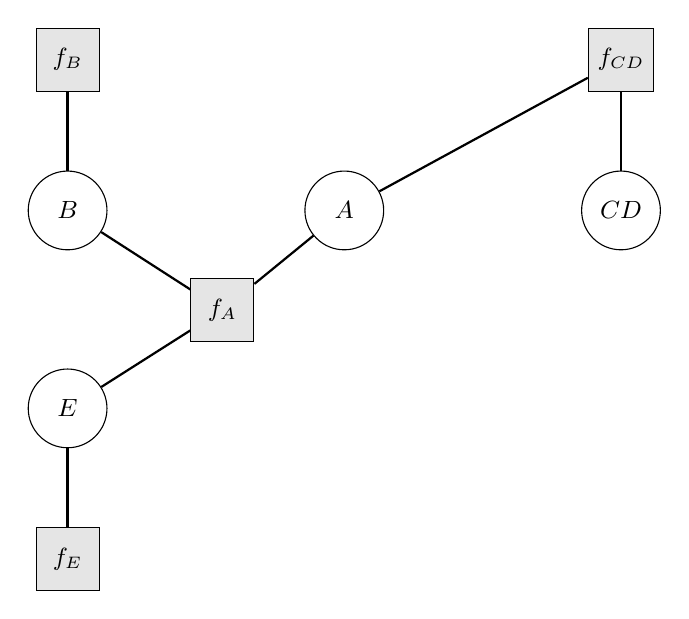
\begin{tikzpicture}[
  var/.style={circle, draw, minimum size=10mm, font=\small},
  fac/.style={rectangle, draw, fill=gray!20, minimum size=8mm, font=\small},
  edge/.style={thick},
  node distance=18mm
]
  % Variable nodes
  \node[var] (B) {$B$};
  \node[var, right=25mm of B] (A) {$A$};
  \node[var, below=15mm of B] (E) {$E$};
  \node[var, right=25mm of A] (CD) {$CD$};

  % Factor nodes
  \node[fac, above=10mm of B] (fB) {$f_B$};
  \node[fac, below=10mm of E] (fE) {$f_E$};
  \node[fac, below right=5mm and 12mm of B] (fA) {$f_A$};
  \node[fac, above=10mm of CD] (fCD) {$f_{CD}$};

  % Edges
  \draw[edge] (B) -- (fB);
  \draw[edge] (E) -- (fE);
  \draw[edge] (B) -- (fA);
  \draw[edge] (E) -- (fA);
  \draw[edge] (A) -- (fA);
  \draw[edge] (A) -- (fCD);
  \draw[edge] (CD) -- (fCD);
\end{tikzpicture}
\end{center}

\noindent Each factor's scope and adjacency:
\begin{center}
\begin{tabular}{llll}
\toprule
\textbf{Factor} & \textbf{Node} & \textbf{Parents} & \textbf{Scope} \\
\midrule
$f_B$ & $B$ & --- & $\{B\}$ \\
$f_E$ & $E$ & --- & $\{E\}$ \\
$f_A$ & $A$ & $B, E$ & $\{A, B, E\}$ \\
$f_{CD}$ & $CD$ & $A$ & $\{CD, A\}$ \\
\bottomrule
\end{tabular}
\end{center}

Variable adjacency: $B \leftrightarrow \{f_B, f_A\}$, \;
$E \leftrightarrow \{f_E, f_A\}$, \;
$A \leftrightarrow \{f_A, f_{CD}\}$, \;
$CD \leftrightarrow \{f_{CD}\}$.

\subsection{Credal Factors (Extreme Points)}

\paragraph{Factor $f_B$: $K(B)$, no parents.}
\begin{center}
\begin{tabular}{lcc}
\toprule
\textbf{Vertex} & $P(B{=}0)$ & $P(B{=}1)$ \\
\midrule
$v_1$ & 0.80 & 0.20 \\
$v_2$ & 0.90 & 0.10 \\
\bottomrule
\end{tabular}
\end{center}

\paragraph{Factor $f_E$: $K(E)$, no parents.}
\begin{center}
\begin{tabular}{lcc}
\toprule
\textbf{Vertex} & $P(E{=}0)$ & $P(E{=}1)$ \\
\midrule
$v_1$ & 0.90 & 0.10 \\
$v_2$ & 0.95 & 0.05 \\
\bottomrule
\end{tabular}
\end{center}

\paragraph{Factor $f_A$: $K(A \mid B, E)$, parents $\{B, E\}$.}
Four parent configurations, each with 2 vertices ($2^4 = 16$ vertex combinations):
\begin{center}
\begin{tabular}{llcc}
\toprule
\textbf{Parent config} & \textbf{Vertex} & $P(A{=}0 \mid \cdot)$ & $P(A{=}1 \mid \cdot)$ \\
\midrule
$B{=}0, E{=}0$ & $v_1$ & 0.9556 & 0.0444 \\
$B{=}0, E{=}0$ & $v_2$ & 1.0000 & 0.0000 \\
\midrule
$B{=}1, E{=}0$ & $v_1$ & 0.0000 & 1.0000 \\
$B{=}1, E{=}0$ & $v_2$ & 1.0000 & 0.0000 \\
\midrule
$B{=}0, E{=}1$ & $v_1$ & 0.0000 & 1.0000 \\
$B{=}0, E{=}1$ & $v_2$ & 1.0000 & 0.0000 \\
\midrule
$B{=}1, E{=}1$ & $v_1$ & 0.0000 & 1.0000 \\
$B{=}1, E{=}1$ & $v_2$ & 1.0000 & 0.0000 \\
\bottomrule
\end{tabular}
\end{center}

\paragraph{Factor $f_{CD}$: $K(CD \mid A)$, parent $\{A\}$.}
Two parent configurations: $A{=}0$ (4 vertices) and $A{=}1$ (11 vertices).
For brevity, we show a subset:
\begin{center}
\begin{tabular}{llcccc}
\toprule
\textbf{Config} & \textbf{Vtx} & $P(CD{=}0)$ & $P(CD{=}1)$ & $P(CD{=}2)$ & $P(CD{=}3)$ \\
\midrule
$A{=}0$ & $v_1$ & 0.00 & 0.00 & 0.00 & 1.00 \\
$A{=}0$ & $v_2$ & 0.00 & 0.00 & 1.00 & 0.00 \\
$A{=}0$ & $v_3$ & 0.00 & 1.00 & 0.00 & 0.00 \\
$A{=}0$ & $v_4$ & 1.00 & 0.00 & 0.00 & 0.00 \\
\midrule
$A{=}1$ & $v_1$ & 0.00 & 0.00 & 0.30 & 0.70 \\
$A{=}1$ & $v_2$ & 0.00 & 0.30 & 0.00 & 0.70 \\
\multicolumn{2}{l}{$\cdots$ (9 more)} \\
\bottomrule
\end{tabular}
\end{center}

There are $4 \times 11 = 44$ vertex combinations for $f_{CD}$.

\subsection{Query: $P(B{=}1)$, No Evidence}

\subsubsection{Iteration 1: Factor-to-Variable Messages}

\paragraph{Message $f_B \to B$.}
Factor $f_B$ has scope $\{B\}$ with no parents and no other variables ($\mathcal{O} = \emptyset$).

\begin{itemize}
\item \textbf{Vertex combinations:} 2 (one per vertex of $K(B)$, since there is only one parent configuration---the empty one).
\item \textbf{Corner-point combinations:} $2^0 = 1$ (no other variables).
\end{itemize}

Computation for each $\mathbf{vc}$:
\begin{align*}
  \mathbf{vc} = (1): \quad & m = v_1 = [0.80,\, 0.20], \quad
  p = m / 1.0 = [0.80,\, 0.20]. \\
  \mathbf{vc} = (2): \quad & m = v_2 = [0.90,\, 0.10], \quad
  p = m / 1.0 = [0.90,\, 0.10].
\end{align*}

Result:
\[
  \mu_{f_B \to B} = \bigl(\,\underbrace{[\,0.80,\; 0.10\,]}_{\mathbf{l} = \min},\;
  \underbrace{[\,0.90,\; 0.20\,]}_{\mathbf{u} = \max}\,\bigr).
\]

\paragraph{Message $f_E \to E$.} Analogous computation:
\[
  \mu_{f_E \to E} = \bigl(\,[\,0.90,\; 0.05\,],\; [\,0.95,\; 0.10\,]\,\bigr).
\]

\paragraph{Message $f_A \to A$.}
Factor $f_A$ has scope $\{A, B, E\}$, target is $A$, so $\mathcal{O} = \{B, E\}$.
Specializing Equation~\ref{eq:case-general} to this target gives:
\[
  m(A{=}x) = \sum_{\pi \in \{0,1\}^2} P_{\mathbf{vc}}(A{=}x \mid B{=}\pi_B, E{=}\pi_E)
  \cdot \mathbf{q}_B(\pi_B) \cdot \mathbf{q}_E(\pi_E).
\]

In iteration~1, the incoming messages are vacuous: $\mu_{B \to f_A} = ([0,0],[1,1])$,
$\mu_{E \to f_A} = ([0,0],[1,1])$.

\begin{itemize}
\item \textbf{Vertex combinations:} $2^4 = 16$ (2 vertices per each of 4 parent configs).
\item \textbf{Corner-point combinations:} $2^2 = 4$ (lower or upper for $B$ and $E$).
\end{itemize}

When both incoming messages are vacuous, many $(\mathbf{vc}, \mathbf{cc})$ pairs
produce $m = [0, 0]$ (zero total) because $\mathbf{q}_B = [0,0]$ or
$\mathbf{q}_E = [0,0]$ zeroes out the product.
Only $\mathbf{cc} = (1,1)$ (both upper bounds $=[1,1]$) produces nonzero marginals.

\textbf{Detailed example:} $\mathbf{vc} = (1,1,1,1)$ (vertex~1 for all configs),
$\mathbf{cc} = (1,1)$ ($\mathbf{q}_B = [1,1]$, $\mathbf{q}_E = [1,1]$):
\begin{align*}
  m(A{=}0) &= 0.9556 \cdot 1 \cdot 1 + 0.0000 \cdot 1 \cdot 1
              + 0.0000 \cdot 1 \cdot 1 + 0.0000 \cdot 1 \cdot 1 = 0.9556, \\
  m(A{=}1) &= 0.0444 \cdot 1 \cdot 1 + 1.0000 \cdot 1 \cdot 1
              + 1.0000 \cdot 1 \cdot 1 + 1.0000 \cdot 1 \cdot 1 = 3.0444, \\
  p &= [0.9556, 3.0444] / 4.0 = [0.2389,\, 0.7611].
\end{align*}

After scanning all 16 vertex combinations (with $\mathbf{cc} = (1,1)$),
the resulting message is wide because vacuous inputs provide no information.

\paragraph{Message $f_A \to B$.}
Target is $B$ (a parent), $\mathcal{O} = \{A, E\}$. This is Case~2.
With vacuous incoming messages, the message to $B$ is similarly wide.

\paragraph{Messages from $f_{CD}$.}
Factor $f_{CD}$ has scope $\{CD, A\}$ with 44 vertex combinations and $2^1 = 2$
corner-point combinations per target variable. In the first iteration with
vacuous incoming messages, these produce wide bounds.

\subsubsection{Iteration 1: Variable-to-Factor Messages}

After the factor-to-variable messages are computed, the variable-to-factor
messages are updated by \emph{tightening}: each variable sends to a factor
the intersection of messages from all \emph{other} factors.

\paragraph{Message $B \to f_A$.}
Variable $B$ has neighbors $\{f_B, f_A\}$. The message to $f_A$ excludes $f_A$ itself:
\[
  \mu_{B \to f_A} = \mu_{f_B \to B} = \bigl(\,[0.80,\, 0.10],\; [0.90,\, 0.20]\,\bigr).
\]
This is a significant tightening from the vacuous $([0,0],[1,1])$: factor $f_B$
directly constrains $B$'s marginal, and this information is now passed to $f_A$.

\paragraph{Message $E \to f_A$.}
Similarly, $E$ has neighbors $\{f_E, f_A\}$:
\[
  \mu_{E \to f_A} = \mu_{f_E \to E} = \bigl(\,[0.90,\, 0.05],\; [0.95,\, 0.10]\,\bigr).
\]

\paragraph{Message $A \to f_{CD}$.}
Variable $A$ has neighbors $\{f_A, f_{CD}\}$:
\[
  \mu_{A \to f_{CD}} = \mu_{f_A \to A}.
\]

\subsubsection{Iteration 2: Recomputing $f_A \to A$ with Informative Messages}

Now $f_A$ receives informative messages from $B$ and $E$. The computation of
$f_A \to A$ uses:
\begin{align*}
  \mathbf{q}_B &\in \{[0.80,\, 0.10],\; [0.90,\, 0.20]\}, \\
  \mathbf{q}_E &\in \{[0.90,\, 0.05],\; [0.95,\, 0.10]\}.
\end{align*}

\textbf{Detailed example:} $\mathbf{vc} = (1,1,1,1)$, $\mathbf{cc}$: $\mathbf{q}_B = [0.80, 0.10]$,
$\mathbf{q}_E = [0.90, 0.05]$:
\begin{align*}
  m(A{=}0) &= 0.9556 \cdot 0.80 \cdot 0.90 + 0.0000 \cdot 0.10 \cdot 0.90 \\
            &\quad + 0.0000 \cdot 0.80 \cdot 0.05 + 0.0000 \cdot 0.10 \cdot 0.05 = 0.6880, \\
  m(A{=}1) &= 0.0444 \cdot 0.80 \cdot 0.90 + 1.0000 \cdot 0.10 \cdot 0.90 \\
            &\quad + 1.0000 \cdot 0.80 \cdot 0.05 + 1.0000 \cdot 0.10 \cdot 0.05 = 0.1670, \\
  p &= [0.6880,\, 0.1670] / 0.8550 = [\,0.8047,\; 0.1953\,].
\end{align*}

Another example: $\mathbf{vc} = (1,1,1,1)$, $\mathbf{cc}$: $\mathbf{q}_B = [0.90, 0.20]$,
$\mathbf{q}_E = [0.95, 0.10]$:
\begin{align*}
  m(A{=}0) &= 0.9556 \cdot 0.90 \cdot 0.95 + 0.0 \cdot 0.20 \cdot 0.95 \\
            &\quad + 0.0 \cdot 0.90 \cdot 0.10 + 0.0 \cdot 0.20 \cdot 0.10 = 0.8170, \\
  m(A{=}1) &= 0.0444 \cdot 0.90 \cdot 0.95 + 1.0 \cdot 0.20 \cdot 0.95 \\
            &\quad + 1.0 \cdot 0.90 \cdot 0.10 + 1.0 \cdot 0.20 \cdot 0.10 = 0.3380, \\
  p &= [0.8170,\, 0.3380] / 1.1550 = [\,0.7074,\; 0.2926\,].
\end{align*}

As the incoming messages become more informative (tighter intervals), the factor
explores a more constrained space and the message to $A$ tightens accordingly.

\subsubsection{Final Marginal Extraction}

After convergence, the marginal bounds for $B$ are:
\[
  \underline{P}(B{=}x) = \max_{f \in \{f_B, f_A\}} l_{f \to B}(x), \quad
  \overline{P}(B{=}x) = \min_{f \in \{f_B, f_A\}} u_{f \to B}(x).
\]
Factor $f_B$ provides the tightest bounds for $B$ since it directly encodes $K(B)$:
\[
  P(B{=}1) \in [0.10,\; 0.20].
\]

\subsection{Query with Evidence: $P(B{=}1 \mid E{=}1)$}\label{sec:example-evidence}

We now rerun IBP with evidence $E = 1$. According to Section~\ref{sec:evidence},
the outgoing messages from $E$ are clamped to the one-hot indicator for state
$1$:
\[
  \mu_{E \to f_E} \;=\; \mu_{E \to f_A} \;=\; \bigl([0,\, 1],\; [0,\, 1]\bigr),
\]
and $E$ is skipped in every subsequent variable-to-factor update.

\subsubsection{Iteration 1: $f_B \to B$ and $f_E \to E$.}
$f_B$ is not adjacent to $E$, so its outgoing message is identical to the
no-evidence case:
\[
  \mu_{f_B \to B} = \bigl([\,0.80,\; 0.10\,],\; [\,0.90,\; 0.20\,]\bigr).
\]
$f_E \to E$ is also unchanged by the clamping of $\mu_{E \to f_E}$ (the factor
receives evidence on its target; the outgoing message still reflects
$K(E)$). However, this message will be intersected with the clamped
$\mu_{E \to f_E}$ only at the extraction step, so in practice $P(E)$ is pinned
to $[0, 1]$ on state $1$.

\subsubsection{Iteration 1: $f_A \to A$ with $E$ clamped.}
Target is $A$, $\mathcal{O} = \{B, E\}$. In iteration~1, $B$ still
sends the vacuous message $\mu_{B \to f_A} = ([0,0],[1,1])$, but
$\mu_{E \to f_A} = ([0,1], [0,1])$. The corner-point enumeration over
$\mathcal{O}$ now collapses along the $E$ axis since both corners select
$\mathbf{q}_E = [0, 1]$, leaving only the two $B$ corners free. Using
Equation~\ref{eq:case-general}:
\[
  m(A{=}x) = \sum_{\pi_B, \pi_E \in \{0,1\}}
             P_{\mathbf{vc}}(A{=}x \mid B{=}\pi_B, E{=}\pi_E) \cdot
             \mathbf{q}_B(\pi_B) \cdot \underbrace{\mathbf{q}_E(\pi_E)}_{0 \text{ if } \pi_E = 0}.
\]
Only the $\pi_E = 1$ terms survive. With $\mathbf{vc} = (1,1,1,1)$ (vertex~1
for every parent configuration) and $\mathbf{q}_B = [1, 1]$ (the upper corner,
since $B$'s message is vacuous):
\begin{align*}
  m(A{=}0) &= \underbrace{0.9556 \cdot 1 \cdot 0}_{B{=}0,E{=}0}
           + \underbrace{0.0000 \cdot 1 \cdot 0}_{B{=}1,E{=}0}
           + \underbrace{0.0000 \cdot 1 \cdot 1}_{B{=}0,E{=}1}
           + \underbrace{0.0000 \cdot 1 \cdot 1}_{B{=}1,E{=}1} = 0, \\
  m(A{=}1) &= \underbrace{0.0444 \cdot 1 \cdot 0}_{B{=}0,E{=}0}
           + \underbrace{1.0000 \cdot 1 \cdot 0}_{B{=}1,E{=}0}
           + \underbrace{1.0000 \cdot 1 \cdot 1}_{B{=}0,E{=}1}
           + \underbrace{1.0000 \cdot 1 \cdot 1}_{B{=}1,E{=}1} = 2.0, \\
  p &= [0,\; 2.0]/2.0 = [0,\; 1].
\end{align*}
Under $\mathbf{vc} = (2,2,1,1)$ (vertex~2 for $B{=}0,E{=}0$ and $B{=}1,E{=}0$,
vertex~1 for $B{=}0,E{=}1$ and $B{=}1,E{=}1$), the same calculation still gives
$p = [0, 1]$ because the $\pi_E = 0$ terms are zeroed out regardless of the
vertex choice there. Clamping $E{=}1$ drives the marginal of $A$ toward
$A{=}1$: whenever $E{=}1$ forces the child, all surviving vertices in these
configurations have $P(A{=}1 \mid \cdot) = 1.0$ for vertex~1 and $P(A{=}0 \mid
\cdot) = 1.0$ for vertex~2. Combining across vertex combinations yields
$\mu_{f_A \to A} = ([0, 0], [1, 1])$ in iteration~1 --- still wide, because
$B$ is vacuous.

\subsubsection{Iteration 1: $f_A \to B$ with $E$ clamped.}
Target is $B$, $\mathcal{O} = \{A, E\}$. Again $\mathbf{q}_E = [0, 1]$
in both corners, and only parent configurations with $\pi_E = 1$ contribute.
Specializing Equation~\ref{eq:case-general} with $\mathbf{q}_A = [0, 0]$ or $[1, 1]$
(vacuous):
\[
  m(B{=}x) = \sum_{\pi_E = 1}
             \Bigl(\sum_{x_i} P_{\mathbf{vc}}(A{=}x_i \mid B{=}x, E{=}1)
                   \cdot \mathbf{q}_A(x_i)\Bigr) \cdot \mathbf{q}_E(1).
\]
The inner sum over $x_i$ is exactly $\sum_{x_i} \mathbf{q}_A(x_i) \cdot 1$
(since vertex~1 has $P(A{=}1 \mid \cdot) = 1$ and vertex~2 has
$P(A{=}0 \mid \cdot) = 1$ for the two $E{=}1$ rows). The upper corner
$\mathbf{q}_A = [1,1]$ gives $m(B{=}0) = m(B{=}1) = 1$, i.e.\ $p = [0.5, 0.5]$;
the lower corner $\mathbf{q}_A = [0,0]$ zeros out the marginal. Combined with
other vertex combinations, $\mu_{f_A \to B}$ in iteration~1 remains wide.

\subsubsection{Iteration 2: $B \to f_A$ and recomputation.}
By Section~\ref{sec:evidence}, $E$ is skipped in the variable-to-factor phase;
only $B$ (and $A$, $CD$) are updated. $B$'s message to $f_A$ tightens to
$\mu_{B \to f_A} = \mu_{f_B \to B} = ([0.80, 0.10], [0.90, 0.20])$.
Re-executing $f_A \to B$ with this informative $B$ message and the still-clamped
$E$ produces a tighter interval. After message passing converges, the bounds on
$B$ follow from the extraction step applied to evidence-clamped messages:
\[
  \underline{P}(B{=}x \mid E{=}1) = \max_{f \in \{f_B, f_A\}} l_{f \to B}(x),
  \quad
  \overline{P}(B{=}x \mid E{=}1) = \min_{f \in \{f_B, f_A\}} u_{f \to B}(x).
\]
$f_B$ still contributes its prior bounds $[0.10, 0.20]$ on $P(B{=}1)$, while
$f_A$ now carries information about $B$ conditioned on $E{=}1$. On this
polytree the two are consistent and the conditional posterior recovers the
prior:
\[
  P(B{=}1 \mid E{=}1) \in [0.10,\; 0.20],
\]
reflecting the fact that $B$ and $E$ are marginally independent in the alarm
network and the asymmetry of $A$'s CPT does not alter $B$'s marginal under
evidence on $E$ alone.

\subsection{Proofs of Theorem 3 and 4}

The complexity bound of Theorem 3 follows immediately from the size of the messages passed along the edges of the factor graph. 

First, IBP is known to be exact on singly connected structures (ie, trees) \cite{pearl88,dechter-bucket}. Given that $\cL$ is family-realizable there are no cross-family constraints and by Proposition 2 we have that $\DSE = \DLCN$. It follows easily that CVE computes exact marginals with respect to $\DLCN$ if $\cL$ is singly connected. 

%% ================================================================
\section{Detailed Description: Coordinate Descent with Variable Elimination}
\label{sec-full-cdve}
%% ================================================================

\begin{algorithm}[t!]
\caption{Coordinate Descend with Variable Elimination (CDVE)}
\label{alg:cdve}
\begin{multicols}{2}
\begin{algorithmic}[1]
\Require LCN $\cL$ with variables $\{X_1, \ldots, X_n\}$, evidence $\mathbf{E} = \mathbf{e}$, iterations $T$
\Ensure Bounds $[\underline{P}(Z{=}z|\be),\; \overline{P}(Z{=}z|\be)]$ for
        non-evidence variables $Z$ and states $z$
\Statex
\State Build credal network $\cC$ using chain graph factorization of $\cL$

\For{each non-evidence variable $Z$}
  \State $\underline{\mathbf{p}},\, \overline{\mathbf{p}} \gets \mathbf{1},\, \mathbf{0}$
         \Comment{component-wise over $D_Z$}
  \For{$\mathrm{sense} \in \{\min, \max\}$}
    \State $P(X_i \mid \pi_i) \gets \mathrm{centroid}(\mathrm{ext}\,\kr{X_i \mid \pi_i})$
    \State $p^* \gets \mathrm{VE}(\{P(X_i|\pi_i)\},\, Z,\, \mathbf{y})$
    \For{sweep $t = 1, \dots, T$}
      \For{each $(X_i, \pi_i)$}
        \State $v^\star \gets \arg\,\mathrm{sense}_{v \in \mathrm{ext}\,K(X_i \mid \pi_i)}\;
               \mathrm{VE}(\{P\}[P(X_i \mid \pi_i){\gets}v],\, Z,\, \mathbf{y})(z)$
        \Statex \hspace{3em}\Comment{$z$ = target state this run is tracking}
        \State \textbf{if} $v^\star$ strictly improves $p^*(z)$
               \textbf{then} $P(X_i \mid \pi_i) \gets v^\star$,\;
               $p^* \gets \mathrm{VE}(\{P\},\, Z,\, \mathbf{y})$
      \EndFor
      \State \textbf{if} sweep made no change \textbf{then break}
    \EndFor
    \State $\underline{\mathbf{p}} \gets \min(\underline{\mathbf{p}},\, p^*)$,\quad
           $\overline{\mathbf{p}} \gets \max(\overline{\mathbf{p}},\, p^*)$
  \EndFor
  \State \Return $[\underline{p}(z),\, \overline{p}(z)]$ for every $z \in D_Z$
\EndFor
\end{algorithmic}
\end{multicols}
\end{algorithm}

Our third approach is called Coordinate Descent with Variable Elimination (CDVE) and is described by Algorithm \ref{alg:cdve}. CDVE extends the ApproxLP method \cite{antonucci2015approxlp} that reformulates credal marginal inference as a multilinear program and solves it via coordinate descent. 

Specifically, for every non-evidence variable $Z$, the CDVE runs coordinate descent twice --- once with sense $\min$ and once with sense $\max$. Each run starts by initializing all $P(X_i \mid \pi_i)$ at the centroid of their respective credal sets and computing $p^* = \mathrm{VE}(\{P\}, Z, \mathbf{y})$, the full posterior vector on $D_Z$ under these fixed distributions. A \emph{sweep} then visits every $(X_i, \pi_i)$: for each vertex $v \in \mathrm{ext}\,K(X_i \mid \pi_i)$, it temporarily sets $P(X_i \mid \pi_i) \gets v$, re-evaluates $\mathrm{VE}$, and accepts $v$ (strictly, else rejects) if the target component $p^*(z)$ moves in the sense's direction. Sweeps repeat until one produces no improvement or the cap $T$ is reached. Because
each $\mathrm{VE}$ call returns a full vector, the two runs together yield componentwise bounds $[\underline{p}(z), \overline{p}(z)]$ for every state $z \in D_Z$ simultaneously. Evidence variables are skipped by a point-mass shortcut. The output is \emph{inner bounds} --- coordinate descent explores only a subset of feasible vertex combinations, so the returned interval is
contained in the true interval. 

\subsection{Detailed Example}
We trace CDVE on the example LCN with variables $B$, $E$, $A$,
$CD$ and the DAG $B \to A$, $E \to A$, $A \to CD$.

\subsubsection{Factor Graph}

\begin{center}
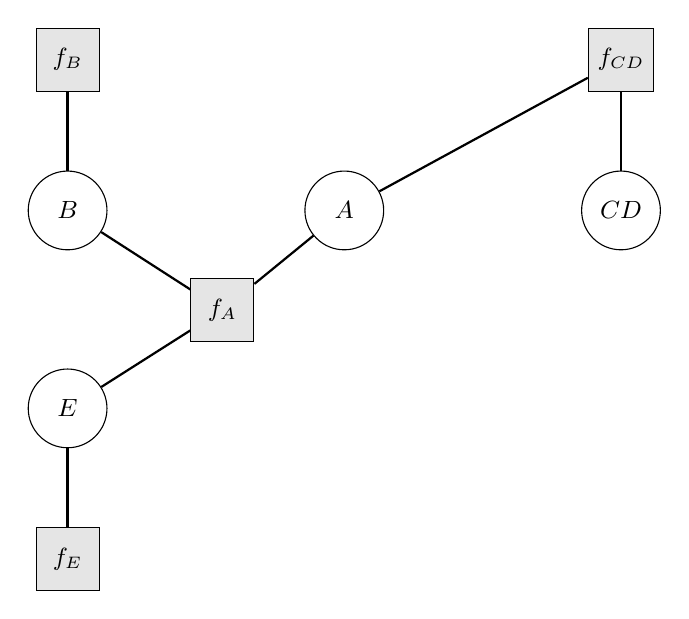
\begin{tikzpicture}[
  var/.style={circle, draw, minimum size=10mm, font=\small},
  fac/.style={rectangle, draw, fill=gray!20, minimum size=8mm, font=\small},
  edge/.style={thick},
  node distance=18mm
]
  \node[var] (B) {$B$};
  \node[var, right=25mm of B] (A) {$A$};
  \node[var, below=15mm of B] (E) {$E$};
  \node[var, right=25mm of A] (CD) {$CD$};
  \node[fac, above=10mm of B] (fB) {$f_B$};
  \node[fac, below=10mm of E] (fE) {$f_E$};
  \node[fac, below right=5mm and 12mm of B] (fA) {$f_A$};
  \node[fac, above=10mm of CD] (fCD) {$f_{CD}$};
  \draw[edge] (B) -- (fB);
  \draw[edge] (E) -- (fE);
  \draw[edge] (B) -- (fA);
  \draw[edge] (E) -- (fA);
  \draw[edge] (A) -- (fA);
  \draw[edge] (A) -- (fCD);
  \draw[edge] (CD) -- (fCD);
\end{tikzpicture}
\end{center}

\subsubsection{Credal Factors (Extreme Points)}

\paragraph{$f_B$: $K(B)$.} $v_1 = [0.80, 0.20]$, \; $v_2 = [0.90, 0.10]$.

\paragraph{$f_E$: $K(E)$.} $v_1 = [0.90, 0.10]$, \; $v_2 = [0.95, 0.05]$.

\paragraph{$f_A$: $K(A \mid B, E)$.} 4 parent configs, 2 vertices each:

\begin{center}
\begin{tabular}{llcc}
\toprule
\textbf{Config} & \textbf{Vtx} & $P(A{=}0)$ & $P(A{=}1)$ \\
\midrule
$B{=}0, E{=}0$ & $v_1$ & 0.9556 & 0.0444 \\
$B{=}0, E{=}0$ & $v_2$ & 1.0000 & 0.0000 \\
\midrule
$B{=}1, E{=}0$ & $v_1$ & 0.0000 & 1.0000 \\
$B{=}1, E{=}0$ & $v_2$ & 1.0000 & 0.0000 \\
\midrule
$B{=}0, E{=}1$ & $v_1$ & 0.0000 & 1.0000 \\
$B{=}0, E{=}1$ & $v_2$ & 1.0000 & 0.0000 \\
\midrule
$B{=}1, E{=}1$ & $v_1$ & 0.0000 & 1.0000 \\
$B{=}1, E{=}1$ & $v_2$ & 1.0000 & 0.0000 \\
\bottomrule
\end{tabular}
\end{center}

\paragraph{$f_{CD}$: $K(CD \mid A)$.} $A{=}0$: 4 vertices; $A{=}1$: 11 vertices (see companion documents for full listing).

\subsubsection{Query 1: $P(B{=}1)$, No Evidence}

\paragraph{Step 1: Initialization.}
Each distribution is set to the center (average) of its credal set:
\begin{align*}
  P(B) &= \tfrac{1}{2}([0.80, 0.20] + [0.90, 0.10]) = [0.85,\; 0.15], \\
  P(E) &= \tfrac{1}{2}([0.90, 0.10] + [0.95, 0.05]) = [0.925,\; 0.075], \\
  P(A \mid B{=}0, E{=}0) &= \tfrac{1}{2}([0.9556, 0.0444] + [1.0, 0.0]) = [0.9778,\; 0.0222].
\end{align*}
(Other parent configs for $A$ are similarly averaged.)

\paragraph{Step 2: Initial evaluation.}
Run VE with these fixed distributions:
\[
  P(B{=}1) = 0.1500 \quad \text{(the center value for $B$).}
\]

\paragraph{Step 3: Coordinate descent (sense = $\min$).}

\textbf{Iteration 0:}

\emph{Try variable $B$, config $()$:}
\begin{itemize}
  \item Set $P(B) = v_1 = [0.80, 0.20]$, run VE: $P(B{=}1) = 0.2000$.
        Worse than $0.1500$ $\to$ reject.
  \item Set $P(B) = v_2 = [0.90, 0.10]$, run VE: $P(B{=}1) = 0.1000$.
        Better $\to$ \textbf{accept}. Update incumbent: $p^* = 0.1000$.
\end{itemize}

\emph{Try variable $E$, config $()$:}
\begin{itemize}
  \item $v_1 = [0.90, 0.10]$: VE gives $P(B{=}1) = 0.1000$. No improvement.
  \item $v_2 = [0.95, 0.05]$: VE gives $P(B{=}1) = 0.1000$. No improvement.
\end{itemize}

Since $B$ is a root node, $P(B)$ directly determines $P(B{=}1)$ regardless of
other distributions. The algorithm correctly identifies $v_2 = [0.90, 0.10]$ as the
minimizer in one iteration.

\emph{Other variables ($A$, $CD$)} have no effect on $P(B{=}1)$ after $B$'s vertex is fixed.

\textbf{Iteration 1:} No improvement found $\to$ converged.

\textbf{Result (min):} $\underline{P}(B{=}1) = 0.1000$.

\paragraph{Coordinate descent (sense = $\max$).}
Analogous: selecting $v_1 = [0.80, 0.20]$ gives $\overline{P}(B{=}1) = 0.2000$.
Converges in 1 iteration.

\paragraph{Final result:}
\[
  \boxed{P(B{=}1) \in [0.1000,\; 0.2000].}
\]

\subsubsection{Query 2: $P(A{=}1 \mid B{=}0, E{=}0)$}

\paragraph{Initialization.}
With evidence $B{=}0, E{=}0$, the only relevant parent config for $A$ is $(B{=}0, E{=}0)$.
The initial center distribution is:
\[
  P(A \mid B{=}0, E{=}0) = [0.9778,\; 0.0222].
\]

\paragraph{Initial evaluation.}
VE with fixed distributions and evidence gives $P(A{=}1 \mid B{=}0, E{=}0) = 0.0222$.

\paragraph{Coordinate descent (sense = $\min$).}

\emph{Try $A$, config $(B{=}0, E{=}0)$:}
\begin{itemize}
  \item $v_1 = [0.9556, 0.0444]$: VE gives $P(A{=}1) = 0.0444$. Worse $\to$ reject.
  \item $v_2 = [1.0000, 0.0000]$: VE gives $P(A{=}1) = 0.0000$. Better $\to$ \textbf{accept}.
\end{itemize}

Converged: $\underline{P}(A{=}1 \mid B{=}0, E{=}0) = 0.0000$.

\paragraph{Coordinate descent (sense = $\max$).}

\emph{Try $A$, config $(B{=}0, E{=}0)$:}
\begin{itemize}
  \item $v_1 = [0.9556, 0.0444]$: $P(A{=}1) = 0.0444$. Better $\to$ \textbf{accept}.
  \item $v_2 = [1.0, 0.0]$: $P(A{=}1) = 0.0000$. Worse $\to$ reject.
\end{itemize}

Converged: $\overline{P}(A{=}1 \mid B{=}0, E{=}0) = 0.0444$.

\paragraph{Final result:}
\[
  \boxed{P(A{=}1 \mid B{=}0, E{=}0) \in [0.0000,\; 0.0444].}
\]

\subsection{Proof of Theorem 5}
The complexity bound follows easily since the inner computation is done by variable elimination which is exponential in the treewidth $w^*$ of the network \cite{dechter-bucket}.

%% ================================================================
\section{Detailed Description of the \textsc{CJT} Algorithm}
\label{sec-full-cjt}
%% ================================================================


\textsc{CJT} proceeds in four steps. It builds a cluster tree over the atoms
from the family scopes of the chain graph \eqref{eq:factor}; it assigns every
sentence and every non-redundant independence assertion to a cluster containing
its scope; it writes a single constraint system whose variables are one
distribution per cluster; and it reads the query off a cluster containing it,
minimizing and maximizing over that system. Algorithm~\ref{alg:cjt} states the
procedure; Section~\ref{sec:nlp} writes the constraint system formally.

The only input the algorithm takes from the chain graph is the collection of
family \emph{scopes} $\{\ch_v\cup\pa_v\}_v$, together with the LCN's own
sentences and assertions. It never forms the local credal sets $K_{v,\pi}$ of
\eqref{eq:se}, and never enumerates their extreme points. This is the structural
reason its target is $\DLCN$ rather than $\DSE$: neither Gap~A nor Gap~B can
arise from a construction that does not build the objects in which those gaps
live.

Throughout, $\mathcal C$ denotes the clusters, $A(C)\subseteq\mathbf V$ the atoms
of cluster $C$, $S_{CD}=A(C)\cap A(D)$ the separator on a tree edge, and
\begin{equation}\label{eq:width}
  w+1=\max_{C\in\mathcal C}|A(C)|,
\end{equation}
so $w$ is the treewidth of the triangulated graph and $w+1$ the largest cluster
measured in atoms. Cluster sizes are always reported in atoms below.

\begin{algorithm}[t]
\caption{\textsc{CJT}: marginal bounds at treewidth cost}
\label{alg:cjt}
\begin{algorithmic}[1]
\Require sentences $\Sigma$, LMC assertions $\Lambda$, family scopes $\mathcal F$,
  evidence $e$, width budget $b$
\Ensure $[\lo P(a\mid e),\ \hi P(a\mid e)]$ for every atom $a\notin\atoms(e)$
\State $\mathcal S\gets\mathcal F\cup\{\atoms(s):s\in\Sigma\text{ cross-family}\}$
  \Comment{assertions do not augment}
\State $T\gets\textsc{BucketTree}(\mathcal S,\textsc{MinFillOrder}(\mathcal S))$;
  \ $A(C)\gets\bigcup_{v\in C}\atoms(v)$
  \Comment{RIP holds \hfill [H1]}
\State remove subsumed leaves; \ $S_{CD}\gets A(C)\cap A(D)$ for each edge
\ForAll{$s\in\Sigma$}
  \Comment{every sentence must be hosted \hfill [H2]}
  \State host $s$ on a cluster $C$ with $\atoms(s)\subseteq A(C)$, if one exists
\EndFor
\If{$\max_C|A(C)|>b$ \textbf{or} some $s\in\Sigma$ was not hosted}
  \State \Return $\textsc{Direct}(a,e)$ for every atom $a\notin\atoms(e)$
    \Comment{$2^n$, uncertified; Rem.~\ref{rem:oracle}}
\EndIf
\ForAll{$\iota=(X\indep Y\mid S)\in\Lambda$}
  \Comment{three-way triage \hfill [H3]}
  \If{$S$ separates $X$ from $Y$ in $G^\ast$} \State skip $\iota$
    \Comment{entailed by the separators}
  \ElsIf{$X\cup Y\cup S\subseteq A(C)$ for some $C$} \State host $\iota$ on $C$
  \Else \State drop $\iota$ \Comment{bound stays outer, may be loose}
  \EndIf
\EndFor
\State build $\mathcal G$: \ $q_C\in\Delta(2^{|A(C)|})$,
  \ $q_C\restr S_{CD}=q_D\restr S_{CD}$, \ and \eqref{eq:nlp-t1}--\eqref{eq:nlp-lmc}
  on each host \Comment{once}
\ForAll{atoms $a\notin\atoms(e)$}
  \If{$\{a\}\cup\atoms(e)\subseteq A(C_a)$ for some $C_a$}
    \Comment{objective only \hfill [H4]}
    \State $\lo P\gets\min_{q\in\mathcal G}\readoff_a(q)$, \
      $\hi P\gets\max_{q\in\mathcal G}\readoff_a(q)$
      \Comment{\eqref{eq:nlp-obj}, \eqref{eq:nlp-obj-ev}}
  \Else
    \State $[\lo P,\hi P]\gets\textsc{Direct}(a,e)$
  \EndIf
  \State clamp $[\lo P,\hi P]$ to $[0,1]$
\EndFor
\end{algorithmic}
\end{algorithm}

\subsection{Constructing the cluster tree}\label{sec:algo-jt}

The scopes to be covered are the family scopes, augmented by one clique per
\emph{cross-family sentence} --- a sentence whose atoms fit inside no single
family scope. Augmenting forces such a sentence's atoms to co-occur in a cluster,
which is what guarantees it a host in Section~\ref{sec:algo-host}.

Independence assertions are deliberately \emph{not} used to augment. They are
structural, and a cluster tree with the running-intersection property already
enforces them through its separators (Section~\ref{sec:algo-host}); adding them
as cliques would inflate the width for no gain. A Markov chain, for instance,
would collapse from width~$2$ to a single cluster containing all $n$ atoms.

Given the scopes, an elimination order is computed greedily by \emph{min-fill} on
the interaction graph --- the graph in which two nodes are adjacent when they
co-occur in some scope --- eliminating at each step a vertex whose elimination
adds fewest fill-in edges. Buckets are then formed along that order, each scope
placed in the bucket of the first order variable it contains; a bucket's cluster
is the union of its scopes, and its parent is the first later order variable
appearing in the cluster after the bucket variable is removed. This is standard
bucket elimination, so \textbf{the resulting tree has the running-intersection
property by construction}, discharging hypothesis~H1 of
Theorem~\ref{thm:d5} without further argument.

Each cluster's atom set $A(C)$ is the union of the atoms of its nodes; a compound
node contributes all atoms of its chain component at once, so a cluster may be
wider in atoms than in nodes. Finally, any \emph{leaf} whose atom set is contained
in its parent's is removed, repeatedly: such a leaf is redundant, since the parent
already carries that joint, and removing it is safe because a leaf has no children
to reattach. Only subsumed leaves are removed, so the tree is not claimed to be
minimal --- a non-maximal cluster may survive in the interior.

\subsection{Hosting and the assertion triage}\label{sec:algo-host}

Say a constraint is \emph{hosted} on a cluster $C$ when $\scope(c)\subseteq A(C)$;
by Lemma~\ref{lem:locality} its value is then a function of $q_C$ alone. Hosting
each constraint on a single cluster suffices: separator consistency propagates its
effect to the rest of the tree, as the reconstruction argument of
Theorem~\ref{thm:d5} makes precise.

Every sentence is hosted if it can be. A sentence with no host cannot be
represented exactly on this tree, and the algorithm falls back to the direct
formulation (Section~\ref{sec:algo-solve}).

Independence assertions admit a three-way triage, and this is the algorithm's most
consequential step:
\begin{enumerate}
  \item \textbf{Separator-entailed $\Rightarrow$ omitted.} If the conditioning set
    $S$ separates $X$ from $Y$ in the chordal graph $G^\ast$ (Definition~\ref{def:d5}),
    every separator-consistent family of cluster marginals already satisfies
    $(X\indep Y\mid S)$, so imposing it would be redundant. This is what keeps a
    chain at width~$2$.
  \item \textbf{Hosted $\Rightarrow$ imposed} as the bilinear equalities
    \eqref{eq:lmc} on the host cluster.
  \item \textbf{Neither $\Rightarrow$ dropped.}
\end{enumerate}
Case~3 is the algorithm's only source of looseness, and it is exactly the failure
of hypothesis~H3. The bound remains valid --- the projection half of
Theorem~\ref{thm:d5} requires neither H2 nor H3 --- but it can be strictly loose;
Remark~\ref{rem:d5reading} exhibits an instance where it is.

\subsection{Solving}\label{sec:algo-solve}

The constraint system of Step~3 mentions no query, and every atom lies in some
cluster because each family scope is itself a clique. One system therefore serves
all marginals: per atom, only the objective changes, and two optimizations are
solved. This is the sense in which the construction is \emph{query-independent}.

\paragraph{Global solution.}
The system is nonconvex: the assertion equalities \eqref{eq:nlp-lmc} are bilinear,
and under evidence so is the ratio equality \eqref{eq:nlp-obj-ev}. Exactness in
Theorem~\ref{thm:d5} refers to the global optimum, so the bounds reported here
were computed with a spatial branch-and-bound solver at gap tolerance $0$.

\begin{remark}[A local solver yields an inner bound]\label{rem:ipoptinner}
Solved instead by a local method from a finite set of starting points --- keeping
the smallest minimum and largest maximum found --- the procedure returns a value
no more extreme than the true optimum in each direction. The resulting interval is
therefore contained in the exact one: an \emph{inner} bound in the sense of
Definition~\ref{def:char}, and not a guarantee. Global solution is what makes
Theorem~\ref{thm:d5} applicable.
\end{remark}

\paragraph{Fallback.}
Two conditions divert a query to the direct $2^n$ formulation: some cluster
exceeding the width budget $b$, and a sentence or query having no host. The first
is global to the instance; the second may be local to one atom, arising when that
atom and the evidence share no cluster, i.e.\ when H4 fails for it alone.

\begin{remark}[The fallback is exact in formulation, not in certificate]\label{rem:oracle}
The fallback optimizes the true $2^n$ program over $\DLCN$, but by a local method,
so its output carries no global guarantee and can be over-tight. Conversely, on
instances where the $2^n$ formulation is solvable but its global solver fails to
certify some endpoint, the cluster program of Section~\ref{sec:nlp} is often the
more reliable route to a bound, even at $n$ small enough for the joint to be
written down.
\end{remark}

A failed optimization is reported as the corresponding vacuous endpoint ($0$ for a
minimum, $1$ for a maximum): uninformative, never unsound. If every marginal
returns vacuous, the instance or the evidence is likely inconsistent.

\subsection{Complexity}\label{sec:algo-complexity}

\emph{Variables.} One per cluster state, so by \eqref{eq:width}
\begin{equation}\label{eq:cost}
  \sum_{C\in\mathcal C}2^{|A(C)|}\;=\;O\!\bigl(n\,2^{w+1}\bigr),
\end{equation}
since $|\mathcal C|=O(n)$, plus one auxiliary scalar per atom under evidence.
Against $2^n$ for the direct formulation, this is the algorithm's reason for
being: the cost is exponential in the treewidth, not in the number of atoms.

\emph{Constraints.} There are $|\mathcal C|$ normalization equalities;
$\sum_{(C,D),\,S_{CD}\ne\varnothing}2^{|S_{CD}|}=O(n2^{w})$ separator equalities;
two rows per hosted sentence; and, per hosted assertion $(X\indep Y\mid S)$,
\begin{equation}\label{eq:lmcrows}
  2^{|Y|}\cdot\max\bigl(1,2^{|S|}\bigr)\quad\text{equalities.}
\end{equation}

\begin{remark}[Which rows are nonconvex, and why the width bound survives]\label{rem:counting}
(a) Only the assertion equalities \eqref{eq:nlp-lmc} and, under evidence, the
ratio equality \eqref{eq:nlp-obj-ev} are nonconvex. The cleared Type-2 rows
\eqref{eq:nlp-t2} are \emph{linear} in $q$, since $\ell$ and $u$ are constants.
Consequently an instance with no evidence and no hosted assertion yields a
\emph{linear} program --- which is exactly the situation in
Section~\ref{sec:cjt-example}, despite that instance being loopy.
(b) The count \eqref{eq:lmcrows} appears unbounded in $|Y|$, but a \emph{hosted}
assertion satisfies $X\cup Y\cup S\subseteq A(C)$, so it contributes at most
$2^{w+1}$ rows and \eqref{eq:cost} is unaffected. An assertion with a wide $Y$ is
precisely one that the triage of Section~\ref{sec:algo-host} either discharges
structurally or drops.
\end{remark}

Per atom the cost is two optimizations over the shared system, hence $2|\mathbf V|$
in total.

\section{The nonlinear program}\label{sec:nlp}

Fix a cluster $C$ and index the $2^{|A(C)|}$ assignments of $A(C)$ by
$i$, writing $\omega^C_i$ for the $i$-th. For a formula $\varphi$ with
$\atoms(\varphi)\subseteq A(C)$ let $A^{(C)}_\varphi\in\{0,1\}^{2^{|A(C)|}}$ be
its indicator vector, $A^{(C)}_\varphi[i]=\mathbf 1[\omega^C_i\models\varphi]$,
and abbreviate $\langle v,q_C\rangle=\sum_i v_iq_{C,i}$; thus
$\langle A^{(C)}_\varphi,q_C\rangle=P(\varphi)$ whenever $q_C$ is the marginal of
a joint on $A(C)$.

\paragraph{Variables and normalization.}
One distribution per cluster,
\begin{equation}\label{eq:nlp-var}
  q_C\in[0,1]^{2^{|A(C)|}},\qquad
  \sum_{i=0}^{2^{|A(C)|}-1}q_{C,i}=1
  \qquad\forall C\in\mathcal C .
\end{equation}
There are no separator variables, no per-family conditional variables and no
global joint variable; the tree structure enters only through the equalities
below.

\paragraph{Marginalization.}
Let $\pi_{C\to S}$ map a state of $C$ to its restriction to $S\subseteq A(C)$,
and define the $0/1$ aggregation matrix
\begin{equation}\label{eq:nlp-M}
  M^{C\to S}_{r,j}=\mathbf 1\bigl[\pi_{C\to S}(j)=r\bigr],
  \qquad\text{so}\qquad
  \bigl(M^{C\to S}q_C\bigr)[r]=(q_C\restr S)(r).
\end{equation}

\paragraph{Separator consistency.}
For every edge with a non-empty separator, the two endpoints must agree on it:
\begin{equation}\label{eq:nlp-sep}
  \sum_{j:\,\pi_{C\to S}(j)=r}q_{C,j}
  \;=\;\sum_{k:\,\pi_{D\to S}(k)=r}q_{D,k}
  \qquad\forall(C,D)\in E,\ \forall r\in\{0,\dots,2^{|S_{CD}|}-1\},
\end{equation}
equivalently $q_C\restr S_{CD}=q_D\restr S_{CD}$: linear equalities,
$2^{|S_{CD}|}$ per edge. No messages are computed; the consistency conditions are
imposed simultaneously with all others, which is what distinguishes this
formulation from message passing.

\paragraph{Sentences.}
A Type-1 sentence hosted on $C_h\supseteq\atoms(\varphi)$ contributes
\begin{equation}\label{eq:nlp-t1}
  \ell\;\le\;\bigl\langle A^{(C_h)}_{\varphi},\,q_{C_h}\bigr\rangle\;\le\;u,
\end{equation}
and a Type-2 sentence contributes the cleared pair
\begin{equation}\label{eq:nlp-t2}
  \ell\,\bigl\langle A^{(C_h)}_{\psi},q_{C_h}\bigr\rangle
  \;\le\;\bigl\langle A^{(C_h)}_{\varphi\wedge\psi},q_{C_h}\bigr\rangle
  \;\le\;u\,\bigl\langle A^{(C_h)}_{\psi},q_{C_h}\bigr\rangle .
\end{equation}
No division appears, and consistently with Remark~\ref{rem:cleared} the rows
\eqref{eq:nlp-t2} are vacuously satisfied when $P(\psi)=0$: a Type-2 sentence
constrains nothing on a null conditioning event.

\paragraph{Independence assertions.}
For a hosted $(X\indep Y\mid S)$ with $X=\{x\}$, one equality per configuration
$(\mathbf y,\mathbf s)$. With $S\ne\varnothing$, writing the four indicators for
$\{x{=}1,Y{=}\mathbf y,S{=}\mathbf s\}$, $\{S{=}\mathbf s\}$,
$\{x{=}1,S{=}\mathbf s\}$, $\{Y{=}\mathbf y,S{=}\mathbf s\}$ as
$A_a,A_b,A_c,A_d$:
\begin{equation}\label{eq:nlp-lmc}
  \langle A_a,q_{C_h}\rangle\,\langle A_b,q_{C_h}\rangle
  -\langle A_c,q_{C_h}\rangle\,\langle A_d,q_{C_h}\rangle=0 ,
\end{equation}
which is \eqref{eq:lmc} verbatim; and with $S=\varnothing$ the marginal form
$\langle A_a,q\rangle-\langle A_b,q\rangle\langle A_c,q\rangle=0$ for
$P(x,\mathbf y)=P(x)P(\mathbf y)$. These rows are bilinear, hence nonconvex, and
are the reason a global solver is required.

Two features of this encoding matter. First, only the $x{=}1$ slice is needed:
with $(\mathbf y,\mathbf s)$ fixed a binary $X$ has one degree of freedom, so the
$x{=}0$ equality follows. Second, the configurations $\mathbf y$ must range over
\emph{whole} assignments of $Y$. Replacing $(X\indep Y\mid S)$ by the pairwise
family $\{(X\indep t\mid S)\}_{t\in Y}$ is strictly weaker for $|Y|\ge2$ ---
pairwise independence does not imply joint independence --- and under-constrains
the program, yielding spuriously loose bounds.

\paragraph{Objective.}\label{sec:nlp-obj}
Let $C_a$ be a cluster containing the query atom $a$ and all evidence atoms
(hypothesis H4). Without evidence the read-off is linear,
\begin{equation}\label{eq:nlp-obj}
  \readoff_a(q)=\bigl\langle A^{(C_a)}_{a=1},\,q_{C_a}\bigr\rangle=P(a{=}1).
\end{equation}
With evidence $e$ the ratio is reformulated with one auxiliary $t\in[0,1]$,
\begin{equation}\label{eq:nlp-obj-ev}
  \readoff_a(q)=t,\qquad
  t\cdot\bigl\langle A^{(C_a)}_{e},q_{C_a}\bigr\rangle
  =\bigl\langle A^{(C_a)}_{a=1}\!\cdot\!A^{(C_a)}_{e},\,q_{C_a}\bigr\rangle ,
\end{equation}
so $t=P(a{=}1\mid e)$ whenever $P(e)>0$. Since $t$ is unconstrained where
$P(e)=0$, a global solver must be prevented from exploiting that degeneracy, and a
denominator floor
\begin{equation}\label{eq:nlp-floor}
  \bigl\langle A^{(C_a)}_{e},q_{C_a}\bigr\rangle\;\ge\;\varepsilon
\end{equation}
is imposed for a small $\varepsilon>0$. Remark~\ref{rem:denfloor} shows this
floor is a soundness hypothesis, not a numerical convenience.

\paragraph{The program.}
Collecting \eqref{eq:nlp-var}--\eqref{eq:nlp-obj-ev},
\begin{equation}\label{eq:nlp-all}
\begin{aligned}
\lo P(a),\ \hi P(a)\;=\;\min/\max\quad &\readoff_a(q)\\
\text{s.t.}\quad
&\textstyle\sum_i q_{C,i}=1,\quad q_{C,i}\in[0,1] && \forall C\in\mathcal C\\
&q_C\restr S_{CD}=q_D\restr S_{CD} && \forall (C,D)\in E,\ S_{CD}\ne\varnothing\\
&\text{\eqref{eq:nlp-t1}, \eqref{eq:nlp-t2}} && \forall\text{ hosted sentence}\\
&\text{\eqref{eq:nlp-lmc}} && \forall\text{ hosted assertion.}
\end{aligned}
\end{equation}

\subsection{A worked example}\label{sec:cjt-example}

We work \texttt{examples/ktree\_fr\_k2\_n4\_example.lcn} completely. It is a
$k$-tree with $k=2$ on four atoms --- \emph{loopy} after moralization, so the
example is not a degenerate singly-connected case --- yet small enough that every
variable and every constraint can be written down.

\subsubsection{The instance}

\begin{align*}
s_0:&\quad 0.084382 \le P(x_1) \le 0.684382\\
s_1:&\quad 0.01 \le P(\lnot x_2 \mid \lnot x_1) \le 0.572656\\
s_2:&\quad 0.092785 \le P(x_3 \mid x_1\wedge x_2) \le 0.692785\\
s_3:&\quad 0.068242 \le P(x_0 \mid x_1\wedge x_3) \le 0.668242
\end{align*}
The chain-graph families, in construction order, are
\[
  x_1\mid\varnothing,\qquad x_2\mid x_1,\qquad x_3\mid x_1,x_2,\qquad
  x_0\mid x_1,x_3,
\]
and the Local Markov Condition yields exactly one assertion,
\[
  (x_0\indep x_2\mid x_1,x_3).
\]

\subsubsection{The junction tree}

Min-fill elimination produces four clusters of at most three atoms, arranged in a
path (Figure~\ref{fig:jt}). In the convention \eqref{eq:width} this is
$w+1=3$, i.e.\ treewidth $w=2=k$, as expected for a $k$-tree:
\[
  \underbrace{\{x_3\}}_{C_4}\ -\
  \underbrace{\{x_2,x_3\}}_{C_3}\ -\
  \underbrace{\{x_1,x_2,x_3\}}_{C_2}\ -\
  \underbrace{\{x_1,x_3,x_0\}}_{C_1},
\]
with separators $S_{12}=\{x_1,x_3\}$, $S_{23}=\{x_2,x_3\}$, $S_{34}=\{x_3\}$.
Hosting assigns $s_0,s_3$ to $C_1$ and $s_1,s_2$ to $C_2$.

\begin{figure}[ht]\centering
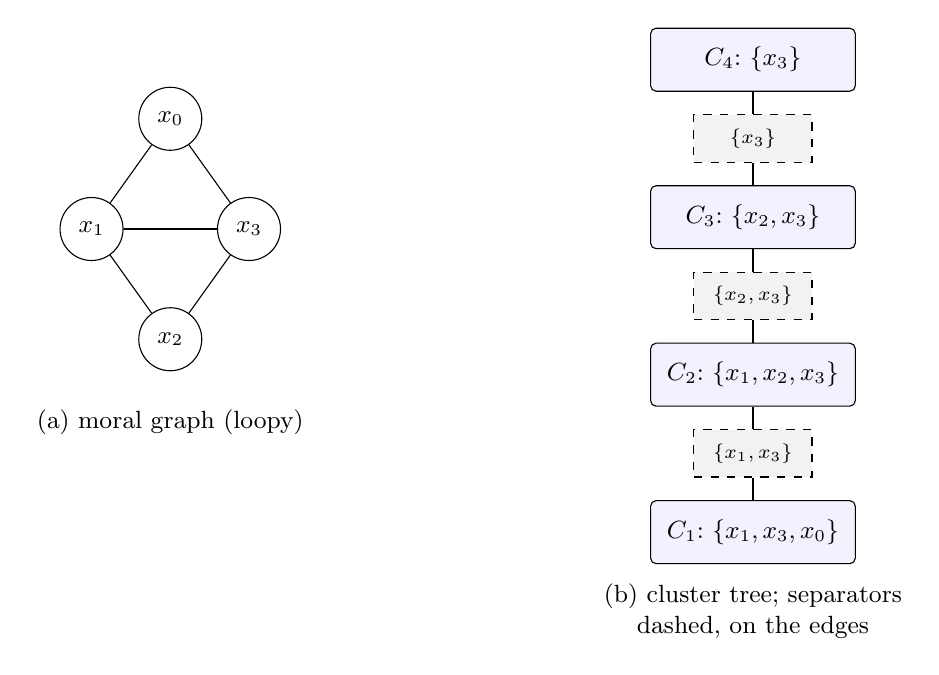
\begin{tikzpicture}[
  atom/.style={circle,draw,minimum size=8mm,inner sep=0pt,font=\small},
  clus/.style={rectangle,draw,rounded corners=2pt,minimum height=8mm,
               minimum width=26mm,inner sep=4pt,font=\small,fill=blue!5},
  sep/.style={rectangle,draw,dashed,minimum height=6mm,minimum width=15mm,
              inner sep=2pt,font=\scriptsize,fill=gray!10},
  panel/.style={font=\small}]

% ---- panel (a): moral graph ----
\begin{scope}[shift={(0,0)}]
  \node[atom] (x0) at (0,3.3)    {$x_0$};
  \node[atom] (x1) at (-1.0,1.9) {$x_1$};
  \node[atom] (x3) at (1.0,1.9)  {$x_3$};
  \node[atom] (x2) at (0,0.5)    {$x_2$};
  \draw (x0)--(x1); \draw (x0)--(x3); \draw (x1)--(x3);
  \draw (x1)--(x2); \draw (x2)--(x3);
  \node[panel] at (0,-0.55) {(a) moral graph (loopy)};
\end{scope}

% ---- panel (b): junction tree, separators as on-edge nodes ----
\begin{scope}[shift={(7.4,0)}]
  \node[clus] (c4) at (0,4.05)  {$C_4{:}\ \{x_3\}$};
  \node[sep]  (s34) at (0,3.05) {$\{x_3\}$};
  \node[clus] (c3) at (0,2.05)  {$C_3{:}\ \{x_2,x_3\}$};
  \node[sep]  (s23) at (0,1.05) {$\{x_2,x_3\}$};
  \node[clus] (c2) at (0,0.05)  {$C_2{:}\ \{x_1,x_2,x_3\}$};
  \node[sep]  (s12) at (0,-0.95){$\{x_1,x_3\}$};
  \node[clus] (c1) at (0,-1.95) {$C_1{:}\ \{x_1,x_3,x_0\}$};
  \draw (c4)--(s34); \draw (s34)--(c3);
  \draw (c3)--(s23); \draw (s23)--(c2);
  \draw (c2)--(s12); \draw (s12)--(c1);
  \node[panel,align=center] at (0,-2.95)
    {(b) cluster tree; separators\\ dashed, on the edges};
\end{scope}
\end{tikzpicture}
\caption{The example instance. Moralization makes $\{x_1,x_2,x_3\}$ and
$\{x_0,x_1,x_3\}$ triangles, so the graph is loopy; the cluster tree nonetheless
has width $2$. The separator $S_{12}=\{x_1,x_3\}$ equals the conditioning set of
the sole assertion $(x_0\indep x_2\mid x_1,x_3)$, which is therefore
separator-entailed and never imposed.}
\label{fig:jt}
\end{figure}

\subsubsection{Separator-entailment discharges the assertion}

The chordal graph $G^\ast$ of Definition~\ref{def:d5} --- two atoms adjacent iff
they co-occur in a cluster --- has edge set
\[
  x_0x_1,\quad x_0x_3,\quad x_1x_2,\quad x_1x_3,\quad x_2x_3,
\]
and in particular $x_0x_2\notin G^\ast$. Deleting $S=\{x_1,x_3\}$ therefore
disconnects $x_0$ from $x_2$: the only paths between them run through $x_1$ or
$x_3$. So $S$ separates $x_0$ from $x_2$ in $G^\ast$, and the sole assertion
$(x_0\indep x_2\mid x_1,x_3)$ is separator-entailed --- case~1 of the triage in
Section~\ref{sec:algo-host}. It is \emph{not} imposed, and the constraint count
below shows zero assertion rows. By Remark~\ref{rem:counting}(a) the program is
consequently a \emph{linear} program, even though the instance is loopy.

This is the mechanism of Theorem~\ref{thm:d5} in its clearest form: the
independence is enforced by the tree's \emph{topology} --- through
Lemma~\ref{lem:rip}'s reconstruction, which produces a joint factorizing over
the chordal graph and hence satisfying its global Markov property --- rather than
by any algebraic row.

\subsubsection{The program in full}

\paragraph{Variables ($22$).}
$q_{C_1}\in\Delta(8)$ over $(x_1,x_3,x_0)$; $q_{C_2}\in\Delta(8)$ over
$(x_1,x_2,x_3)$; $q_{C_3}\in\Delta(4)$ over $(x_2,x_3)$;
$q_{C_4}\in\Delta(2)$ over $(x_3)$. Total $8+8+4+2=22$.

\paragraph{Simplex ($4$).}
$\sum_i q_{C_k,i}=1$ for $k=1,\dots,4$.

\paragraph{Separator consistency ($4+4+2=10$).}
Writing $q_{C}[\,\cdot\,]$ for a cell of cluster $C$, edge $C_1\!-\!C_2$ over
$\{x_1,x_3\}$ gives four equalities,
\[
\begin{aligned}
q_{C_1}[x_1{=}0,x_3{=}0,x_0{=}0]+q_{C_1}[x_1{=}0,x_3{=}0,x_0{=}1]
 &= q_{C_2}[x_1{=}0,x_2{=}0,x_3{=}0]+q_{C_2}[x_1{=}0,x_2{=}1,x_3{=}0],\\
q_{C_1}[x_1{=}0,x_3{=}1,x_0{=}0]+q_{C_1}[x_1{=}0,x_3{=}1,x_0{=}1]
 &= q_{C_2}[x_1{=}0,x_2{=}0,x_3{=}1]+q_{C_2}[x_1{=}0,x_2{=}1,x_3{=}1],\\
q_{C_1}[x_1{=}1,x_3{=}0,x_0{=}0]+q_{C_1}[x_1{=}1,x_3{=}0,x_0{=}1]
 &= q_{C_2}[x_1{=}1,x_2{=}0,x_3{=}0]+q_{C_2}[x_1{=}1,x_2{=}1,x_3{=}0],\\
q_{C_1}[x_1{=}1,x_3{=}1,x_0{=}0]+q_{C_1}[x_1{=}1,x_3{=}1,x_0{=}1]
 &= q_{C_2}[x_1{=}1,x_2{=}0,x_3{=}1]+q_{C_2}[x_1{=}1,x_2{=}1,x_3{=}1];
\end{aligned}
\]
edge $C_2\!-\!C_3$ over $\{x_2,x_3\}$ gives four more,
\[
  q_{C_2}[x_1{=}0,x_2{=}\beta,x_3{=}\gamma]+q_{C_2}[x_1{=}1,x_2{=}\beta,x_3{=}\gamma]
  = q_{C_3}[x_2{=}\beta,x_3{=}\gamma],
  \qquad \beta,\gamma\in\{0,1\};
\]
and edge $C_3\!-\!C_4$ over $\{x_3\}$ gives two,
\[
  q_{C_3}[x_2{=}0,x_3{=}\gamma]+q_{C_3}[x_2{=}1,x_3{=}\gamma]
  = q_{C_4}[x_3{=}\gamma],\qquad \gamma\in\{0,1\}.
\]

\paragraph{Sentence rows ($8$).}
On $C_1$, from $s_0$ (Type-1) and $s_3$ (Type-2, cleared per
\eqref{eq:nlp-t2}):
\[
\begin{aligned}
0.084382&\le\bigl\langle A^{(C_1)}_{x_1},q_{C_1}\bigr\rangle\le 0.684382,\\
0.068242\,\bigl\langle A^{(C_1)}_{x_1\wedge x_3},q_{C_1}\bigr\rangle
&\le\bigl\langle A^{(C_1)}_{x_0\wedge x_1\wedge x_3},q_{C_1}\bigr\rangle
\le 0.668242\,\bigl\langle A^{(C_1)}_{x_1\wedge x_3},q_{C_1}\bigr\rangle .
\end{aligned}
\]
On $C_2$, from $s_1$ and $s_2$ (both Type-2):
\[
\begin{aligned}
0.01\,\bigl\langle A^{(C_2)}_{\lnot x_1},q_{C_2}\bigr\rangle
&\le\bigl\langle A^{(C_2)}_{\lnot x_2\wedge\lnot x_1},q_{C_2}\bigr\rangle
\le 0.572656\,\bigl\langle A^{(C_2)}_{\lnot x_1},q_{C_2}\bigr\rangle,\\
0.092785\,\bigl\langle A^{(C_2)}_{x_1\wedge x_2},q_{C_2}\bigr\rangle
&\le\bigl\langle A^{(C_2)}_{x_3\wedge x_1\wedge x_2},q_{C_2}\bigr\rangle
\le 0.692785\,\bigl\langle A^{(C_2)}_{x_1\wedge x_2},q_{C_2}\bigr\rangle .
\end{aligned}
\]

\paragraph{Independence rows ($0$).}
None, by separator-entailment as argued above.

\paragraph{Totals.}
$22$ variables and $22$ constraints ($4$ simplex, $10$ separator, $8$ sentence,
$0$ LMC), against a joint formulation's $2^4=16$ variables. The example is
deliberately small enough that the treewidth formulation is not yet a saving; the
saving is asymptotic, $O(n2^{w+1})$ against $2^n$, and Table~\ref{tab:contrast}
shows the same machinery on two five-atom instances.

\subsubsection{Results}

Solving \eqref{eq:nlp-all} for each atom with SCIP (global, gap $0$) and
comparing against the independent $2^n$ global engine:

\begin{center}\small
\begin{tabular}{@{}lcccc@{}}
\toprule
engine & $P(x_0)$ & $P(x_1)$ & $P(x_2)$ & $P(x_3)$ \\
\midrule
direct $2^n$ formulation, global & $[0,1]$ & $[0.084382,0.684382]$
  & $[0.134877,0.996844]$ & $[0,1]$ \\
\textsc{CJT} (SCIP)              & $[0,1]$ & $[0.084382,0.684382]$
  & $[0.134877,0.996844]$ & $[0,1]$ \\
\bottomrule
\end{tabular}
\end{center}

\noindent The two solvers agree on every atom to every digit reported, with all
eight of the reference optimizations certified at optimality gap $0$. \textsc{CJT} reports maximum
cluster $3$ atoms, and a total time of about $1.8$\,s.

The vacuous $[0,1]$ on $x_0$ and $x_3$ is genuine rather than a solver artifact,
and the independent oracle confirms it: no sentence constrains $P(x_3)$ except
through conditioning events that can themselves be driven to probability zero,
at which point \eqref{eq:nlp-t2} becomes vacuous (Remark~\ref{rem:cleared}) and
frees the atom. Setting $P(x_1\wedge x_3)=0$ likewise releases $s_3$ and hence
$x_0$. Both endpoints are thus attained by feasible witnesses.

The separator marginals attained at an optimum make the mechanism concrete.
Table~\ref{tab:msgs} lists them at the maximizer of $P(x_1)$. Both endpoints of
every edge agree on these values by \eqref{eq:nlp-sep}; this is the calibrated
family of cluster marginals that Lemma~\ref{lem:rip} reassembles into a joint of
$\DLCN$ attaining the bound.

\begin{table}[ht]\centering\small
\caption{Separator marginals $q_C\restr S$ at the maximizer of $P(x_1)$, listed
over the assignments of $S$. Both clusters incident to an edge realize the same
vector, by \eqref{eq:nlp-sep}.}\label{tab:msgs}
\begin{tabular}{@{}llcccc@{}}
\toprule
edge & separator $S$ & \multicolumn{4}{c}{$q\restr S$ by assignment of $S$}\\
\midrule
$C_1\!-\!C_2$ & $\{x_1,x_3\}$ & $00{:}\,0.3125$ & $01{:}\,0.0032$
  & $10{:}\,0.6844$ & $11{:}\,0.0000$\\
$C_2\!-\!C_3$ & $\{x_2,x_3\}$ & $00{:}\,0.6844$ & $01{:}\,0.0032$
  & $10{:}\,0.3125$ & $11{:}\,0.0000$\\
$C_3\!-\!C_4$ & $\{x_3\}$     & $0{:}\,0.9968$  & $1{:}\,0.0032$
  & & \\
\bottomrule
\end{tabular}
\end{table}


\subsection{Exactness}\label{sec:theory}

This section states and proves the guarantees. The development is closed: it uses
only Lemma~\ref{lem:locality} from Section~\ref{sec:prelim} and
Lemma~\ref{lem:rip} below, and in particular needs no notion of realizability, no
property of the strong extension, and no result about any other engine.

\begin{definition}[Cluster-feasible set, hosting, separator-entailment, read-off]\label{def:d5}
Let $T$ be a clique tree over clusters $\mathcal C$, built by the standard
moralize~$\to$~triangulate~$\to$~clique-tree pipeline, and let $G^\ast$ be the
chordal graph whose maximal cliques are the clusters (two atoms adjacent iff they
co-occur in a cluster).
\begin{itemize}
  \item The \emph{cluster-feasible set} is
  \begin{align*}
    \mathcal G=\bigl\{(q_C)_{C\in\mathcal C}\;:\;
      &q_C\in\Delta(2^{|C|})\ \text{for each }C;\\
      &q_C\restr S=q_D\restr S\ \text{for every edge }(C,D)\in T,\ S=C\cap D;\\
      &\text{every hosted constraint holds on its host cluster}\bigr\}.
  \end{align*}
  \item A constraint $c$ is \emph{hosted} if some cluster
    $C_h\supseteq\scope(c)$ exists; its row is then imposed on $q_{C_h}$'s
    marginal.
  \item An LMC assertion $(X\indep Y\mid S)$ is \emph{separator-entailed} if $S$
    separates $X$ from $Y$ in $G^\ast$.
  \item For a query atom $a$ and evidence $e$ lying together in a cluster $C_a$,
    the \emph{read-off} is $\readoff_a(q)=\sum_{i:a=1}q_{C_a}[i]$ (no evidence),
    or $\readoff_a(q)=\bigl(\sum_{i:a=1,e}q_{C_a}[i]\bigr)/
    \bigl(\sum_{i:e}q_{C_a}[i]\bigr)$ (with evidence).
  \item $\pi(p)=(p\restr C)_{C\in\mathcal C}$ is the \emph{projection} of a joint
    onto the clusters.
\end{itemize}
\end{definition}

The reconstruction direction needs the following lemma, whose usual statement
contains two defects we must repair: it is normally asserted with a
\emph{uniqueness} claim that is false in the presence of zero separator cells,
and the division in the product formula is left unaddressed.

\begin{lemma}[RIP reconstruction, with zeros]\label{lem:rip}
Let $T$ be a clique tree with the running-intersection property over clusters
$\mathcal C$, and let $(q_C)\in\prod_C\Delta(2^{|C|})$ be separator-consistent:
$q_C\restr S=q_D\restr S$ for every edge $(C,D)$ with $S=C\cap D$. Then there
exists a joint distribution $p\in\Delta(2^{\mathbf V})$ with $p\restr C=q_C$ for
every $C\in\mathcal C$, and $p$ factorizes over the cliques of $G^\ast$. Such $p$
is unique if every separator marginal is strictly positive, but \emph{not} in
general.
\end{lemma}

\begin{proof}
Induction on $|\mathcal C|$. If $|\mathcal C|=1$ take $p=q_C$.

Let $|\mathcal C|\ge2$ and pick a leaf cluster $C$ of $T$ with neighbour $D$ and
separator $S=C\cap D$. Let $T'=T-C$; by the running-intersection property
$C\setminus S$ meets no cluster of $T'$, and $(q_{C'})_{C'\in T'}$ is still
separator-consistent, so the inductive hypothesis gives a joint $p'$ over
$\mathbf V'=\bigcup_{C'\in T'}C'$ with $p'\restr C'=q_{C'}$ for all
$C'\in T'$. Note
$p'\restr S=(p'\restr D)\restr S=q_D\restr S=q_C\restr S=:q_S$, using separator
consistency.

Define a conditional kernel on the fresh atoms $C\setminus S$: for each
assignment $s$ of $S$,
\[
  \kappa(\,\cdot\mid s)=
  \begin{cases}
    q_C(\,\cdot\,,s)/q_S(s), & q_S(s)>0,\\
    \delta_{c_0}, & q_S(s)=0,
  \end{cases}
\]
where $c_0$ is any fixed assignment of $C\setminus S$. This is well defined: when
$q_S(s)>0$ the right-hand side is non-negative and sums over $C\setminus S$ to
$q_S(s)/q_S(s)=1$, so it is a distribution. Now set
$p(x)=p'(x_{\mathbf V'})\cdot\kappa(x_{C\setminus S}\mid x_S)$.

$p$ is a distribution: it is non-negative, and summing over $x_{C\setminus S}$
first gives $p'$, which sums to $1$.

\emph{The arbitrary choice is irrelevant.} On $\{x:q_S(x_S)=0\}$ we have
$p'(x_{\mathbf V'})=0$, because $p'\restr S=q_S$ assigns zero mass to that event
and $p'\ge0$. Hence $p$ vanishes there regardless of $\kappa$, so $p$ does not
depend on $c_0$. (This is also the precise sense in which the familiar quotient
formula $p=\prod_C q_C/\prod_{(C,D)}q_S$ is legitimate: a zero separator cell
forces every contributing cluster cell to zero, since $q_S=q_C\restr S$ is a sum
of non-negative $q_C$ entries, so numerator and denominator vanish together and
the term is assigned $0$.)

\emph{Cluster marginals.} For $C'\in T'$: summing $p$ over $x_{C\setminus S}$
gives $p'$, so $p\restr C'=p'\restr C'=q_{C'}$. For $C$ itself:
$p\restr C(c,s)=\bigl(\sum$ of $p$ over $\mathbf V'\setminus S$ at fixed
$x_S=s\bigr)\cdot\kappa(c\mid s)=p'\restr S(s)\,\kappa(c\mid s)
=q_S(s)\kappa(c\mid s)$, which equals $q_C(c,s)$ when $q_S(s)>0$ and equals
$0=q_C(c,s)$ when $q_S(s)=0$. So $p\restr C=q_C$.

\emph{Factorization.} Unwinding the induction, $p$ is a product of one
non-negative factor per cluster (namely $q_C$ or the kernel $\kappa$ derived from
it, each a function of the atoms of that cluster only), hence factorizes over the
cliques of $G^\ast$.

\emph{Non-uniqueness.} If some separator cell $q_S(s)=0$, then
$\kappa(\cdot\mid s)$ was chosen arbitrarily; any other choice yields a joint
with the same cluster marginals, since all such joints vanish on that event.
Hence $p$ is not unique. When all separator marginals are positive the kernels
are forced and the induction determines $p$ uniquely.
\end{proof}

\begin{theorem}[\textsc{CJT} exactness]\label{thm:d5}
Suppose \textup{(H1)} $T$ has the running-intersection property (true by
construction); \textup{(H2)} every LCN sentence is hosted; \textup{(H3)} every
LMC assertion is either hosted or separator-entailed in $G^\ast$; \textup{(H4)}
the query atom and all evidence atoms lie together in some cluster. Then for
every such atom $a$,
\[
  \min_{q\in\mathcal G}\readoff_a(q)=\min_{p\in\DLCN}\readoff_a(\pi(p))=\lo P(a),
  \qquad
  \max_{q\in\mathcal G}\readoff_a(q)=\max_{p\in\DLCN}\readoff_a(\pi(p))=\hi P(a),
\]
and likewise for a conditional query $P(a\mid e)$ subject to
Remark~\ref{rem:denfloor}. Moreover the \emph{projection} half holds without
\textup{(H2)}/\textup{(H3)}, so \textsc{CJT} is always a valid \emph{outer}
bound.
\end{theorem}

\begin{proof}
First note the read-off identity: for any joint $p$,
$\readoff_a(\pi(p))=P_p(a)$ (resp.\ $P_p(a\mid e)$), because $\readoff_a$ sums
the cells of $\pi(p)_{C_a}=p\restr C_a$ in which $a$ (and $e$) hold, which by
definition of a marginal equals $P_p(a)$ (resp.\ the ratio). So both sides
optimize the \emph{same} functional.

\emph{Projection $\DLCN\to\mathcal G$ (needs only H1, H4).} Let $p\in\DLCN$ and
set $q_C:=p\restr C$, i.e.\ $q=\pi(p)$. Each $q_C$ is a distribution (a marginal
of one). Each separator equality holds because both $q_C\restr S$ and
$q_D\restr S$ equal $p\restr S$. Each hosted constraint $c$ holds: by
Lemma~\ref{lem:locality} its value depends on $p$ only through
$p\restr\scope(c)$, and since $\scope(c)\subseteq C_h$ we have
$q_{C_h}\restr\scope(c)=p\restr\scope(c)$, so $c$ holds on the host exactly
because it holds for $p$. Hence $q\in\mathcal G$, with
$\readoff_a(q)=P_p(a)$. Therefore every value achievable over $\DLCN$ is
achievable over $\mathcal G$, giving
$\min_{\mathcal G}\readoff_a\le\min_{\DLCN}$ and
$\max_{\mathcal G}\readoff_a\ge\max_{\DLCN}$: the cluster interval
\emph{contains} the true interval. This is the outer-bound claim, and it used
neither H2 nor H3.

\emph{Reconstruction $\mathcal G\to\DLCN$ (needs H2, H3).} Let
$q\in\mathcal G$. By H1 and Lemma~\ref{lem:rip} there is a joint $p$ with
$p\restr C=q_C$ for every cluster, factorizing over the cliques of $G^\ast$. We
check $p\in\DLCN$.

Sub-scope consistency: if $A\subseteq C$ for some cluster $C$, then
$p\restr A=(p\restr C)\restr A=q_C\restr A$, since marginalizing in stages agrees
with marginalizing at once.

\emph{Hosted constraints} (H2 and the hosted part of H3): let $c$ be hosted on
$C_h$. By the previous paragraph $p\restr\scope(c)=q_{C_h}\restr\scope(c)$, and
$q$ satisfies $c$ on $C_h$ by definition of $\mathcal G$; by
Lemma~\ref{lem:locality} $c$ therefore holds for $p$.

\emph{Separator-entailed LMC} (the other part of H3): let
$(X\indep Y\mid S)$ be separator-entailed, so $S$ separates $X$ from $Y$ in
$G^\ast$. Since $p$ factorizes over the cliques of $G^\ast$, it satisfies the
\emph{global Markov property} of $G^\ast$: factorization implies global Markov
for any undirected graph, and crucially this direction requires \emph{no}
positivity assumption. Global Markov states that if $S$ separates $A$ from $B$ in
$G^\ast$ then $A\indep B\mid S$ under $p$; applying it to the connected
components separated by $S$ and then restricting to the subsets $X$ and $Y$ of
those components (conditional independence is preserved under taking subsets, by
the decomposition property of conditional independence) gives
$X\indep Y\mid S$ under $p$, i.e.\ \eqref{eq:lmc} holds. Note this assertion was
never imposed on $\mathcal G$: it holds automatically for the reconstructed $p$.

Hence $p\in\DLCN$, and $\readoff_a(q)=\readoff_a(\pi(p))=P_p(a)$ because
$\pi(p)=q$ on the host cluster. So every value achievable over $\mathcal G$ is
achievable over $\DLCN$, giving the reverse inequalities. Combined with the
projection half, the optima coincide. For a conditional query, by H4 the read-off
is a functional of the single cluster $C_a$ and both maps preserve $q_{C_a}$, so
the same argument applies verbatim.
\end{proof}


\begin{remark}[The denominator floor is a soundness hypothesis]\label{rem:denfloor}
The conditional read-off is linearized by the auxiliary equality
\eqref{eq:nlp-obj-ev} together with the denominator floor \eqref{eq:nlp-floor}.
The floor is an extra constraint on $\mathcal G$ that $\DLCN$ does not have, so
the projection half of Theorem~\ref{thm:d5} --- and with it the outer-bound
guarantee --- holds only for joints with $P(e)\ge\varepsilon$. If
$\min_{p\in\DLCN}P(e)<\varepsilon$, the returned conditional interval can be
\emph{unsound}. This is a soundness caveat, not merely a tightness one, and it is
the price of admitting conditional queries into a globally solved formulation.
\end{remark}



%% ================================================================
\section{Detailed Experimental Evaluation}
\label{sec-full-results}
%% ================================================================

This appendix reports every measurement behind Section~\ref{sec-experiments}:
all four random families at both scales, and the complete per-instance results
for the two realistic suites. Throughout, the reference is CredalJT and the
budget is $3600$ seconds and $30$\,GB per run.

\subsection{Coverage and exclusions}
\label{sec-coverage}

Not every algorithm completes on every instance, and reading the figures without
this in mind would overstate coverage, since a curve simply stops where its
algorithm ran out of budget. Over the $480$ random instances, ARIEL and IBP
complete essentially all of them, and CredalJT's \texttt{ipopt} backend completes
all of the instances it was run on. The exceptions are concentrated in the
CVE family. Plain CVE, without clustering, is the least scalable: it solves
$35/60$ of \texttt{tree\_small}, $30/60$ of \texttt{polytree\_small} and $24/60$
of \texttt{dag\_small}, but \emph{none} of \texttt{ktree\_small} ($21$ timeouts
and $39$ errors) and none of \texttt{polytree\_large}; on the other three large
families it was not run at all. It is therefore absent from most plots, and where
present it covers only the smallest sizes. Clustering restores coverage at small
scale --- CVE$_{cm}$ and CVE$_{cp}$ solve all $60$ instances of every small
family --- but degrades on the large loopy ones, where CVE$_{cm}$ reaches only
$14/60$ on \texttt{ktree\_large} and $30/60$ on \texttt{dag\_large}. Exact
inference over the $2^n$ joint is viable only at the very smallest sizes
($15/60$ on \texttt{tree\_small}, $13/60$ on \texttt{polytree\_small}, $2/10$ on
the Bayesian-network instances, none of the Supreme Court ones), which is why it
is not used as the reference. Three bookkeeping gaps are worth recording: the
\texttt{ktree\_large} CDVE log holds $58$ records rather than $60$, the Supreme
Court exact-inference log holds $12$ rather than $16$, and the
Bayesian-network CVE log holds $7$ rather than $10$; the corresponding instances
are simply missing rather than failed, and are excluded from the aggregates.

\subsection{Random LCNs}

Figures~\ref{fig:tree-full}--\ref{fig:dag-full} give the error and timing curves
for all four families at both scales. The tables that follow them give the
underlying per-size aggregates; for each family and scale the first table reports
means and the second the corresponding standard deviations over the ten instances
at each size.

\begin{figure}[htbp]
    \centering
    \begin{subfigure}{\linewidth}
        \centering
        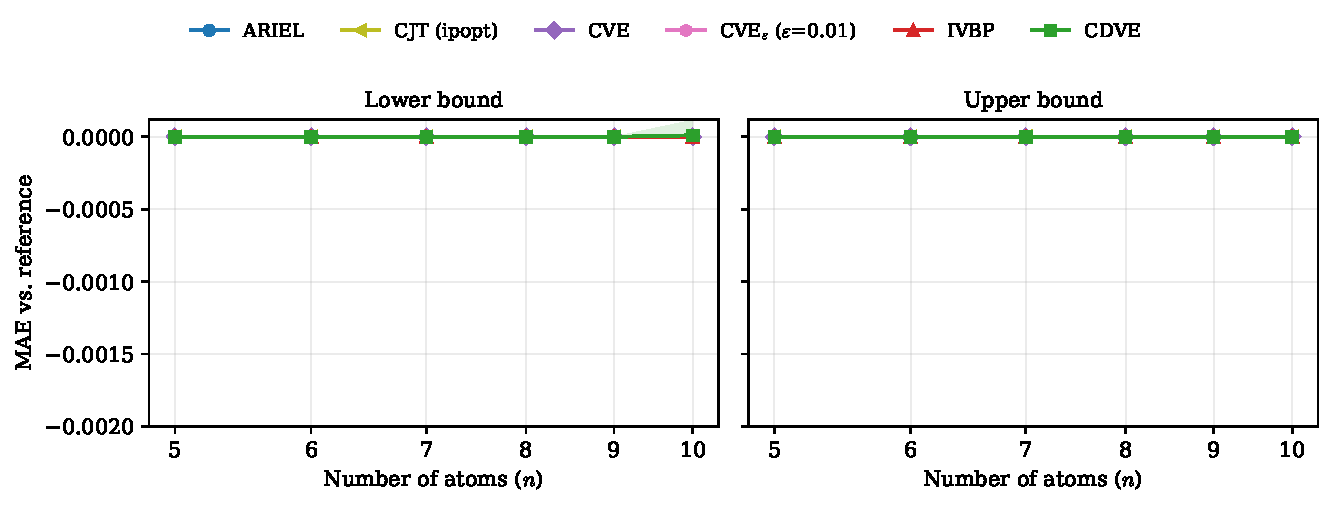
\includegraphics[width=0.9\linewidth]{figs/tree_small_fr_mae.pdf}
        \caption{small, error}
    \end{subfigure}\hfill
    \begin{subfigure}{\linewidth}
        \centering
        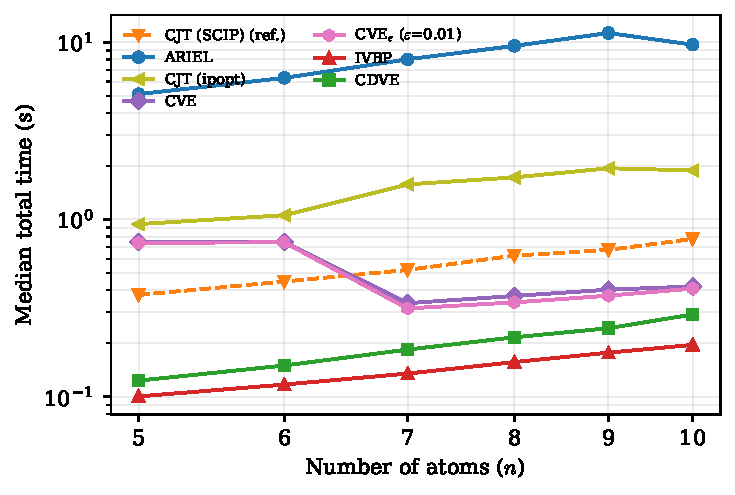
\includegraphics[width=0.5\linewidth]{figs/tree_small_fr_runtime.pdf}
        \caption{small, time}
    \end{subfigure}
    \\[0.3em]
    \begin{subfigure}{\linewidth}
        \centering
        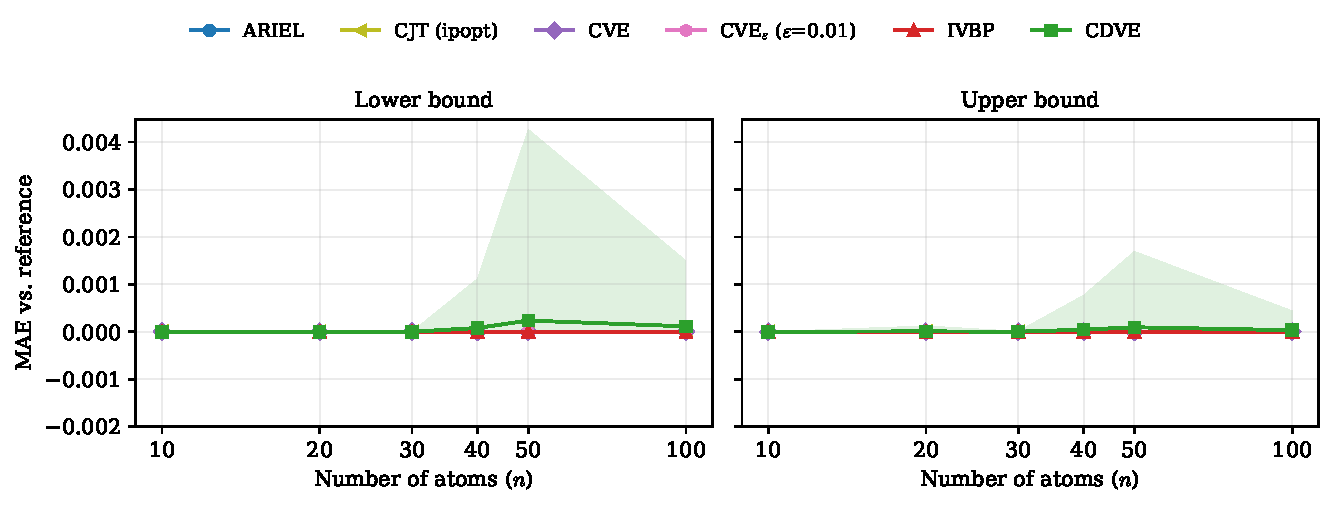
\includegraphics[width=0.9\linewidth]{figs/tree_large_fr_mae.pdf}
        \caption{large, error}
    \end{subfigure}\hfill
    \begin{subfigure}{\linewidth}
        \centering
        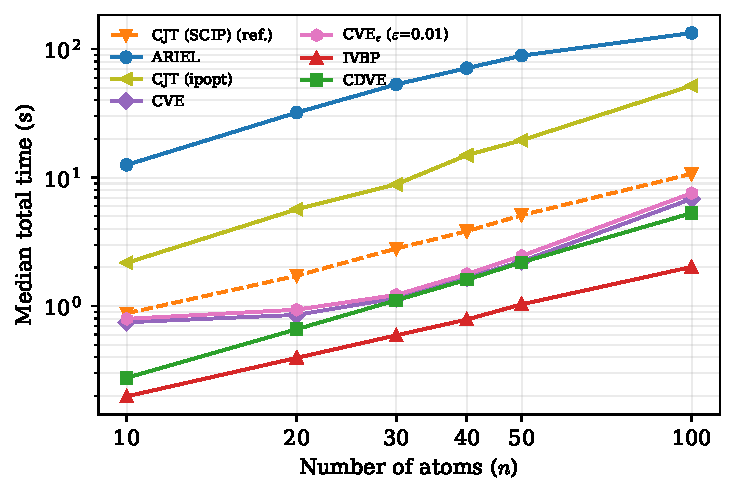
\includegraphics[width=0.5\linewidth]{figs/tree_large_fr_runtime.pdf}
        \caption{large, time}
    \end{subfigure}
    \caption{Random \texttt{tree} LCNs. Singly connected and fully realizable, so
    the credal-network relaxation is tight: ARIEL and IBP are indistinguishable
    from the reference.}
    \label{fig:tree-full}
\end{figure}

\begin{figure}[htbp]
    \centering
    \begin{subfigure}{\linewidth}
        \centering
        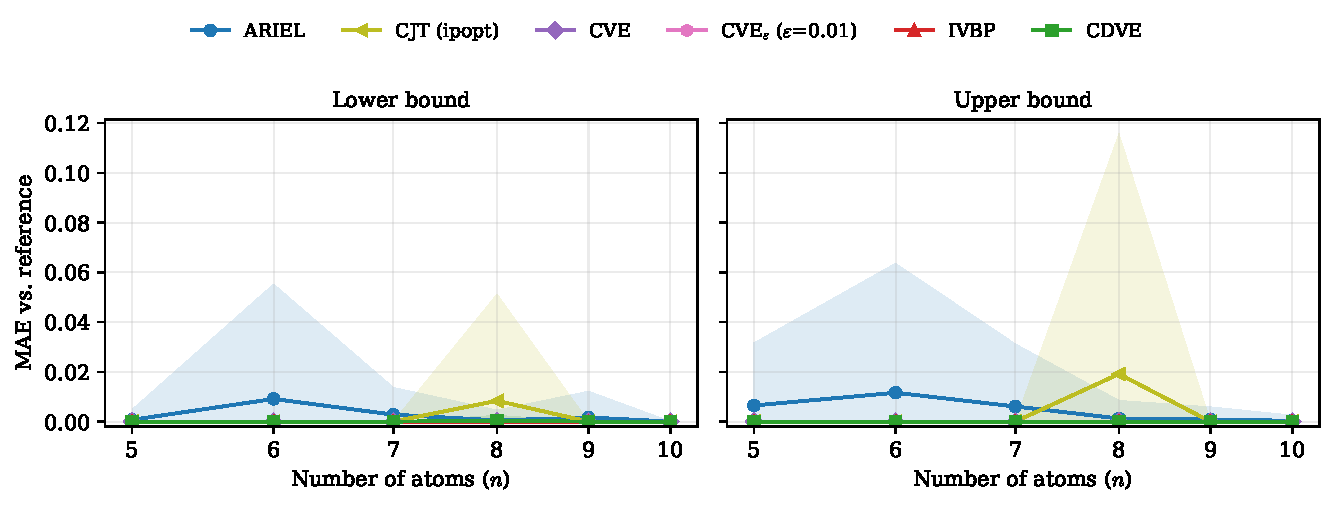
\includegraphics[width=0.9\linewidth]{figs/polytree_small_fr_mae.pdf}
        \caption{small, error}
    \end{subfigure}\hfill
    \begin{subfigure}{\linewidth}
        \centering
        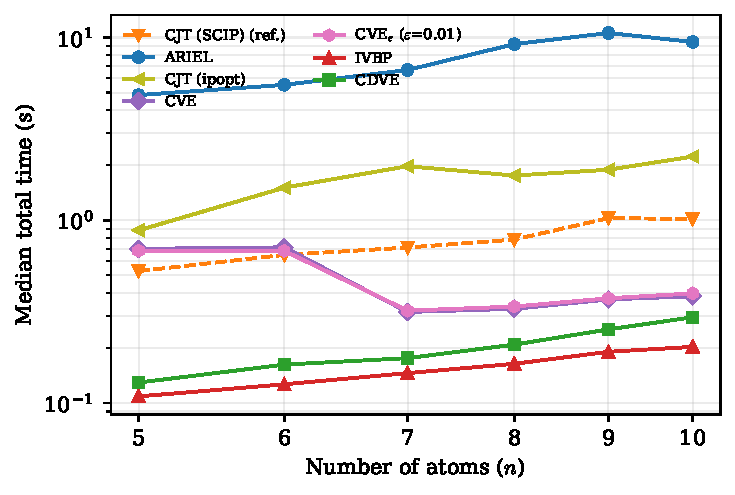
\includegraphics[width=0.5\linewidth]{figs/polytree_small_fr_runtime.pdf}
        \caption{small, time}
    \end{subfigure}
    \\[0.3em]
    \begin{subfigure}{\linewidth}
        \centering
        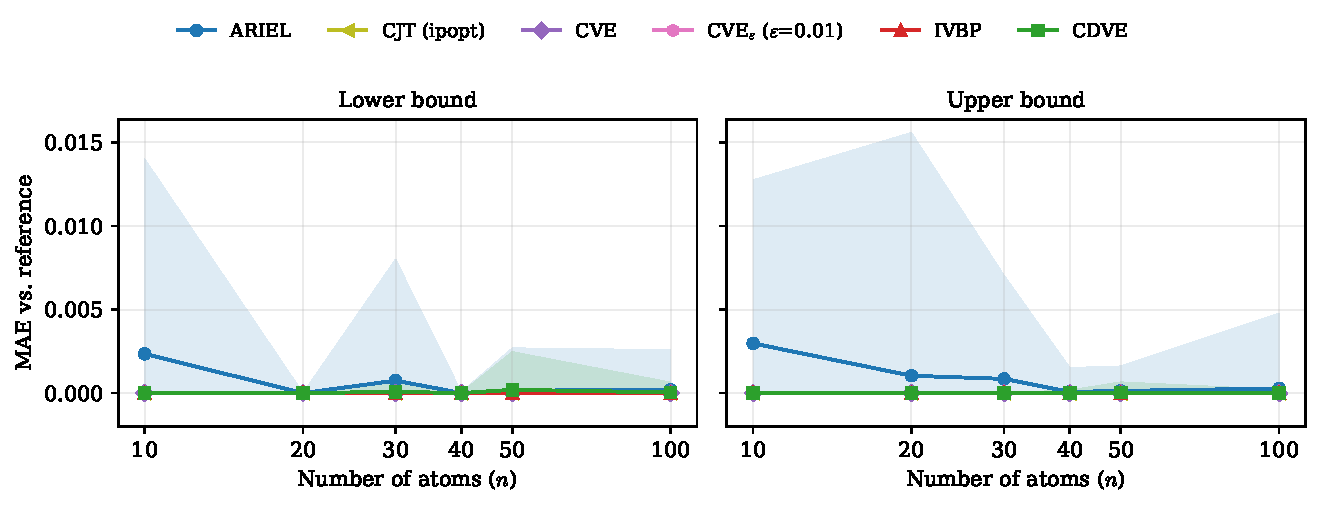
\includegraphics[width=0.9\linewidth]{figs/polytree_large_fr_mae.pdf}
        \caption{large, error}
    \end{subfigure}\hfill
    \begin{subfigure}{0.5\linewidth}
        \centering
        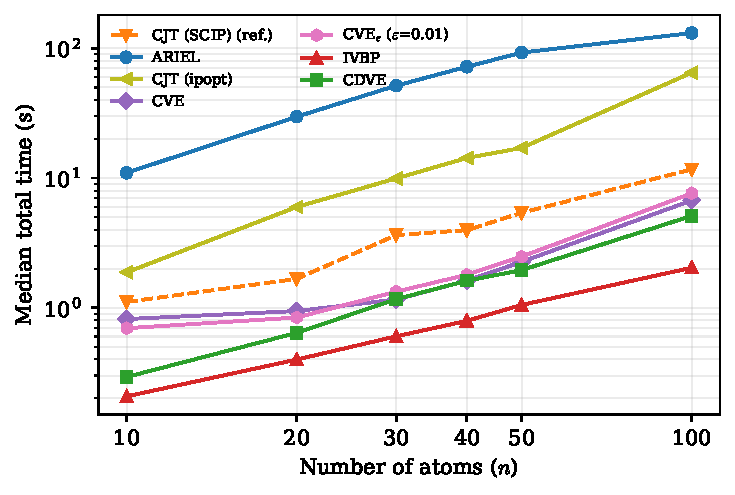
\includegraphics[width=\linewidth]{figs/polytree_large_fr_runtime.pdf}
        \caption{large, time}
    \end{subfigure}
    \caption{Random \texttt{polytree} LCNs. Also singly connected; the residual
    ARIEL error at the small scale comes from instances where the reference
    itself is the tighter engine.}
    \label{fig:polytree-full}
\end{figure}

\begin{figure}[htbp]
    \centering
    \begin{subfigure}{\linewidth}
        \centering
        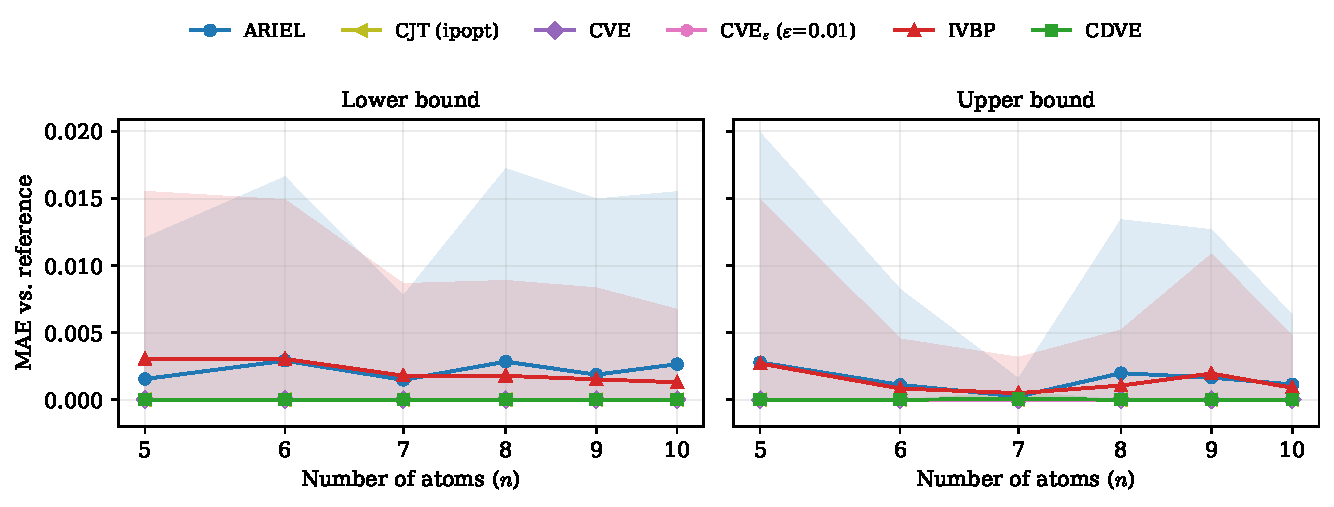
\includegraphics[width=0.9\linewidth]{figs/ktree_small_fr_mae.pdf}
        \caption{small, error}
    \end{subfigure}\hfill
    \begin{subfigure}{\linewidth}
        \centering
        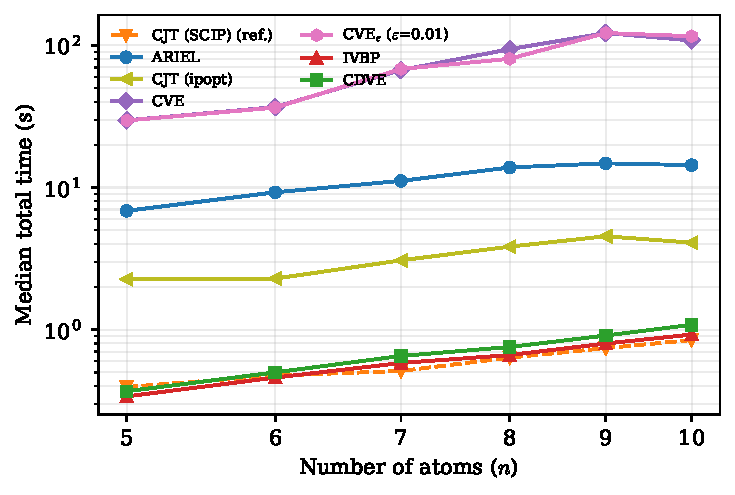
\includegraphics[width=0.5\linewidth]{figs/ktree_small_fr_runtime.pdf}
        \caption{small, time}
    \end{subfigure}
    \\[0.3em]
    \begin{subfigure}{\linewidth}
        \centering
        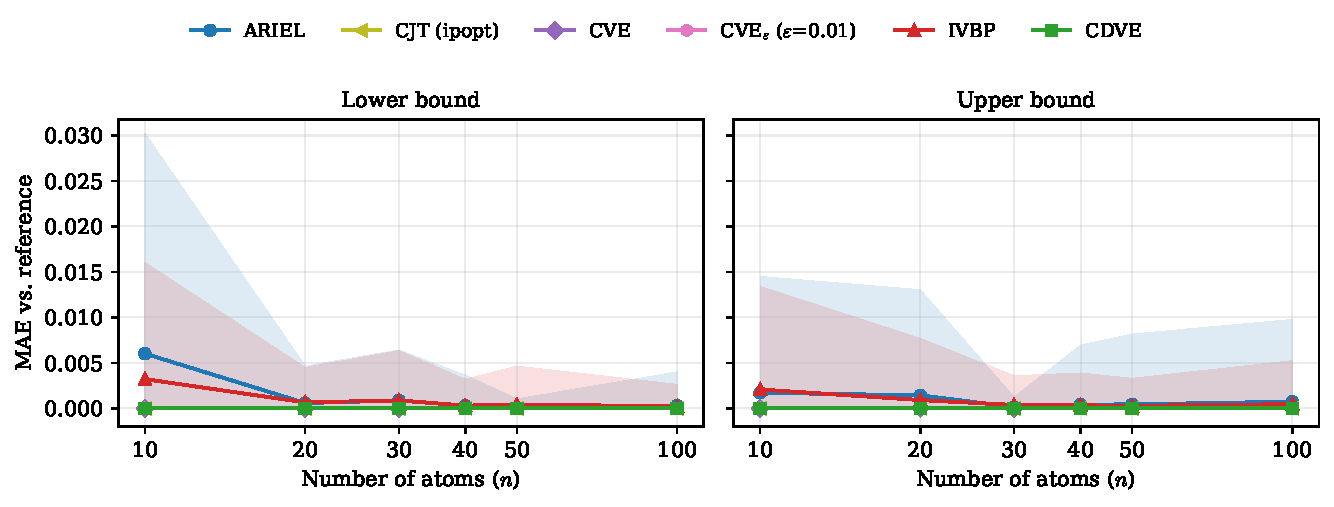
\includegraphics[width=0.9\linewidth]{figs/ktree_large_fr_mae.pdf}
        \caption{large, error}
    \end{subfigure}\hfill
    \begin{subfigure}{\linewidth}
        \centering
        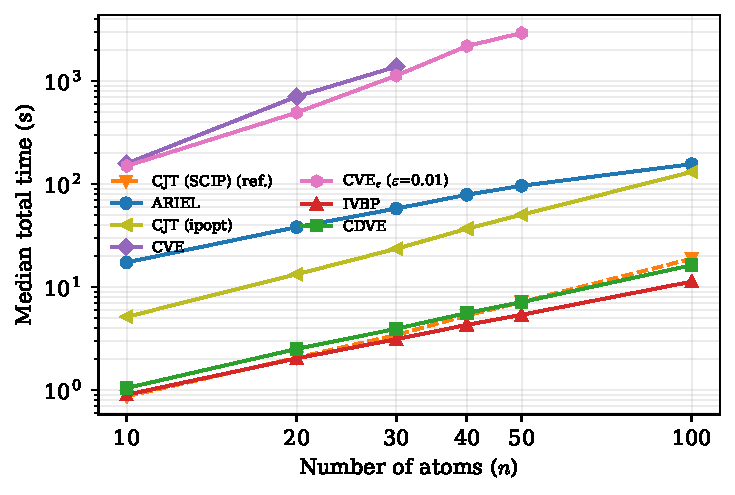
\includegraphics[width=0.5\linewidth]{figs/ktree_large_fr_runtime.pdf}
        \caption{large, time}
    \end{subfigure}
    \caption{Random \texttt{ktree} LCNs ($k{=}3$). Loopy despite bounded
    treewidth, so all credal-network methods give outer bounds only; plain CVE
    solves none of these instances and CVE$_{cm}$ stops after $n{=}20$.}
    \label{fig:ktree-full}
\end{figure}

\begin{figure}[htbp]
    \centering
    \begin{subfigure}{\linewidth}
        \centering
        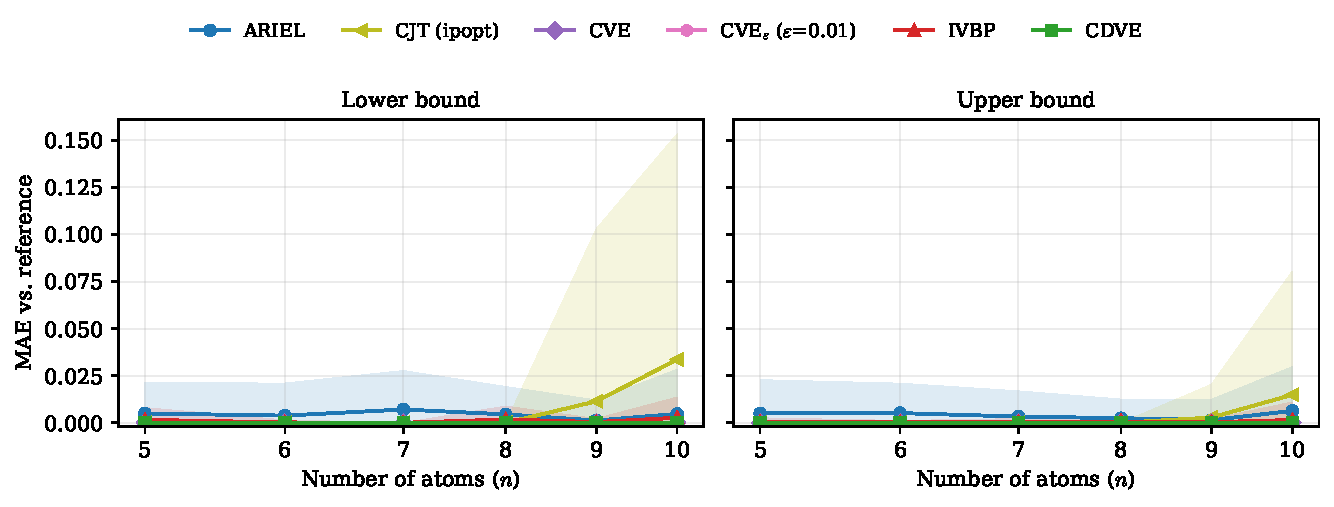
\includegraphics[width=0.9\linewidth]{figs/dag_small_fr_mae.pdf}
        \caption{small, error}
    \end{subfigure}\hfill
    \begin{subfigure}{\linewidth}
        \centering
        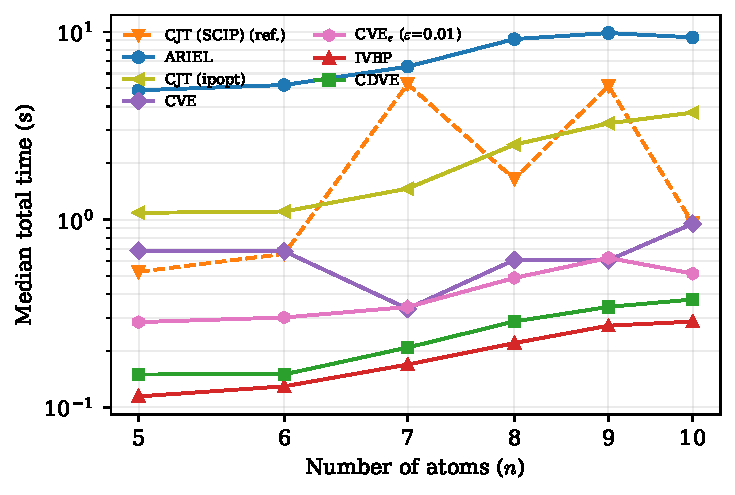
\includegraphics[width=0.5\linewidth]{figs/dag_small_fr_runtime.pdf}
        \caption{small, time}
    \end{subfigure}
    \\[0.3em]
    \begin{subfigure}{\linewidth}
        \centering
        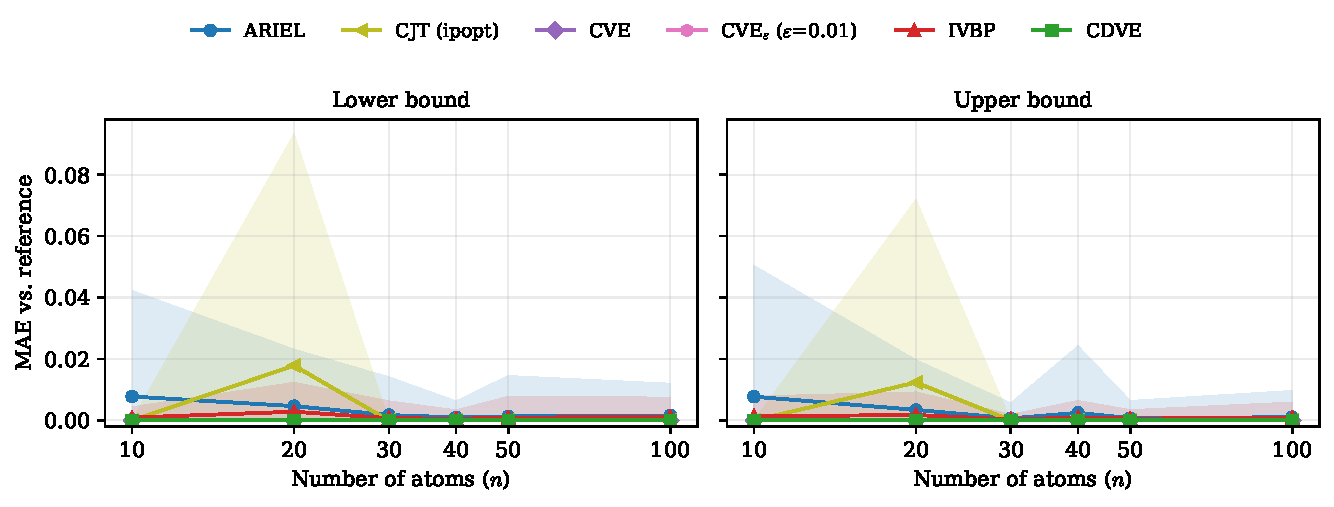
\includegraphics[width=0.9\linewidth]{figs/dag_large_fr_mae.pdf}
        \caption{large, error}
    \end{subfigure}\hfill
    \begin{subfigure}{\linewidth}
        \centering
        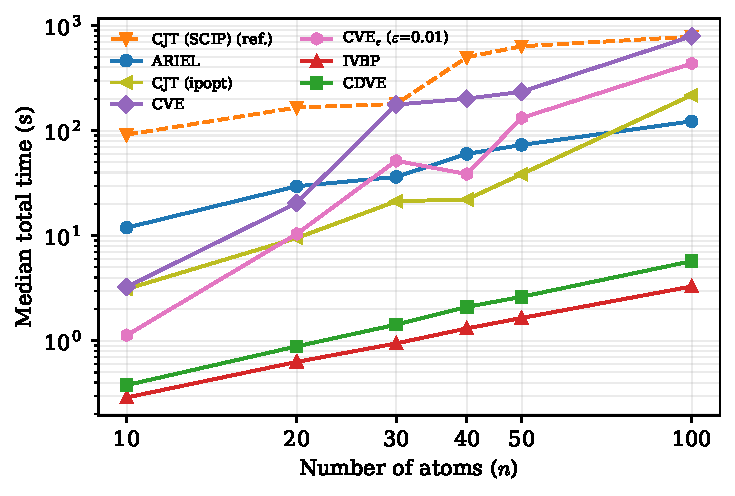
\includegraphics[width=0.5\linewidth]{figs/dag_large_fr_runtime.pdf}
        \caption{large, time}
    \end{subfigure}
    \caption{Random \texttt{dag} LCNs (moralized treewidth $\le 3$, at most two
    parents). The least structured family; CDVE's runtime grows fastest here,
    exceeding $600$ seconds at $n{=}100$.}
    \label{fig:dag-full}
\end{figure}

\clearpage
\begin{table}[htbp]
\centering
\scriptsize
\caption{Random \texttt{tree} LCNs, small scale: errors against the certified CJT (SCIP) endpoints, per size ($10$ instances each). MAE and SD are over atoms; max is the largest error of either endpoint; out/in are the fractions of atoms whose interval contains / is contained in the reference interval (tolerance $10^{-4}$); solved counts give timeouts (t) and memory-outs (m); time is the median total time in seconds over the solved instances. Exact inference over the $2^n$ joint is run only for $n \le 15$; its \emph{solved} instances may hold uncertified (dual) endpoints, hence its large errors.}
\label{tab:full-tree-small}
\begin{tabular}{rlrrrrrrrlr}
\toprule
$n$ & Method & MAE$_l$ & SD$_l$ & MAE$_u$ & SD$_u$ & max & out & in & solved & time \\
\midrule
5 & CJT (SCIP), reference & \multicolumn{7}{l}{certified endpoints 100/100, instances 10/10} & 10/10 & 0.37 \\
 & Exact (SCIP) & 0 & 0 & 0 & 0 & 0 & 1.000 & 1.000 & 10/10 & 9.87 \\
 & Exact (ipopt) & .1687 & .1866 & .1615 & .1559 & .6715 & 0.400 & 0.800 & 10/10 & 27.8 \\
 & ARIEL & 0 & 0 & 0 & 0 & 0 & 1.000 & 1.000 & 10/10 & 5.10 \\
 & CJT (ipopt) & 0 & 0 & 0 & 0 & 0 & 1.000 & 1.000 & 10/10 & 0.94 \\
 & CVE & 0 & 0 & 0 & 0 & 0 & 1.000 & 1.000 & 10/10 & 0.74 \\
 & CVE$_\varepsilon$ ($\varepsilon{=}0.01$) & 0 & 0 & 0 & 0 & 0 & 1.000 & 1.000 & 10/10 & 0.74 \\
 & IVBP & 0 & 0 & 0 & 0 & 0 & 1.000 & 1.000 & 10/10 & 0.10 \\
 & CDVE & 0 & 0 & 0 & 0 & 0 & 1.000 & 1.000 & 10/10 & 0.12 \\
\midrule
6 & CJT (SCIP), reference & \multicolumn{7}{l}{certified endpoints 120/120, instances 10/10} & 10/10 & 0.45 \\
 & Exact (SCIP) & .0449 & .1395 & .0360 & .1247 & .8108 & 0.850 & 0.767 & 10/10 & 1434 \\
 & Exact (ipopt) & .1701 & .2252 & .1537 & .2056 & .9175 & 0.833 & 0.217 & 10/10 & 136 \\
 & ARIEL & 0 & 0 & 0 & 0 & 0 & 1.000 & 1.000 & 10/10 & 6.29 \\
 & CJT (ipopt) & 0 & 0 & 0 & 0 & 0 & 1.000 & 1.000 & 10/10 & 1.06 \\
 & CVE & 0 & 0 & 0 & 0 & 0 & 1.000 & 1.000 & 10/10 & 0.74 \\
 & CVE$_\varepsilon$ ($\varepsilon{=}0.01$) & 0 & 0 & 0 & 0 & 0 & 1.000 & 1.000 & 10/10 & 0.74 \\
 & IVBP & 0 & 0 & 0 & 0 & 0 & 1.000 & 1.000 & 10/10 & 0.12 \\
 & CDVE & 0 & 0 & 0 & 0 & 0 & 1.000 & 1.000 & 10/10 & 0.15 \\
\midrule
7 & CJT (SCIP), reference & \multicolumn{7}{l}{certified endpoints 140/140, instances 10/10} & 10/10 & 0.52 \\
 & Exact (SCIP) & .0923 & .1538 & .1085 & .2136 & .9478 & 0.971 & 0.229 & 10/10 & 3246 \\
 & Exact (ipopt) & .0760 & .1396 & .1131 & .2321 & .9478 & 1.000 & 0.232 & 8/10 (2t) & 390 \\
 & ARIEL & 0 & 0 & 0 & 0 & 0 & 1.000 & 1.000 & 10/10 & 8.02 \\
 & CJT (ipopt) & 0 & 0 & 0 & 0 & 0 & 1.000 & 1.000 & 10/10 & 1.58 \\
 & CVE & 0 & 0 & 0 & 0 & 0 & 1.000 & 1.000 & 10/10 & 0.34 \\
 & CVE$_\varepsilon$ ($\varepsilon{=}0.01$) & 0 & 0 & 0 & 0 & 0 & 1.000 & 1.000 & 10/10 & 0.31 \\
 & IVBP & 0 & 0 & 0 & 0 & 0 & 1.000 & 1.000 & 10/10 & 0.13 \\
 & CDVE & 0 & 0 & 0 & 0 & 0 & 1.000 & 1.000 & 10/10 & 0.18 \\
\midrule
8 & CJT (SCIP), reference & \multicolumn{7}{l}{certified endpoints 160/160, instances 10/10} & 10/10 & 0.63 \\
 & Exact (SCIP) & .1010 & .1789 & .1187 & .2176 & .8828 & 1.000 & 0.050 & 10/10 & 3277 \\
 & Exact (ipopt) & .0869 & .1339 & .1233 & .2225 & .7944 & 1.000 & 0.054 & 7/10 (3t) & 2211 \\
 & ARIEL & 0 & 0 & 0 & 0 & 0 & 1.000 & 1.000 & 10/10 & 9.54 \\
 & CJT (ipopt) & 0 & 0 & 0 & 0 & 0 & 1.000 & 1.000 & 10/10 & 1.73 \\
 & CVE & 0 & 0 & 0 & 0 & 0 & 1.000 & 1.000 & 10/10 & 0.37 \\
 & CVE$_\varepsilon$ ($\varepsilon{=}0.01$) & 0 & 0 & 0 & 0 & 0 & 1.000 & 1.000 & 10/10 & 0.34 \\
 & IVBP & 0 & 0 & 0 & 0 & 0 & 1.000 & 1.000 & 10/10 & 0.16 \\
 & CDVE & 0 & 0 & 0 & 0 & 0 & 1.000 & 1.000 & 10/10 & 0.22 \\
\midrule
9 & CJT (SCIP), reference & \multicolumn{7}{l}{certified endpoints 180/180, instances 10/10} & 10/10 & 0.67 \\
 & Exact (SCIP) & .0971 & .1825 & .0937 & .1759 & .9416 & 1.000 & 0.222 & 10/10 & 3371 \\
 & Exact (ipopt) & -- & -- & -- & -- & -- & -- & -- & 0/10 (10t) & -- \\
 & ARIEL & 0 & 0 & 0 & 0 & 0 & 1.000 & 1.000 & 10/10 & 11.3 \\
 & CJT (ipopt) & 0 & 0 & 0 & 0 & 0 & 1.000 & 1.000 & 10/10 & 1.95 \\
 & CVE & 0 & 0 & 0 & 0 & 0 & 1.000 & 1.000 & 10/10 & 0.40 \\
 & CVE$_\varepsilon$ ($\varepsilon{=}0.01$) & 0 & 0 & 0 & 0 & 0 & 1.000 & 1.000 & 10/10 & 0.37 \\
 & IVBP & 0 & 0 & 0 & 0 & 0 & 1.000 & 1.000 & 10/10 & 0.18 \\
 & CDVE & 0 & 0 & 0 & 0 & 0 & 1.000 & 1.000 & 10/10 & 0.24 \\
\midrule
10 & CJT (SCIP), reference & \multicolumn{7}{l}{certified endpoints 200/200, instances 10/10} & 10/10 & 0.78 \\
 & Exact (SCIP) & .0641 & .1512 & .1071 & .1919 & .8389 & 1.000 & 0.167 & 9/10 (1t) & 3066 \\
 & Exact (ipopt) & -- & -- & -- & -- & -- & -- & -- & 0/10 (10t) & -- \\
 & ARIEL & 0 & 0 & 0 & 0 & 0 & 1.000 & 1.000 & 10/10 & 9.69 \\
 & CJT (ipopt) & 0 & 0 & 0 & 0 & 0 & 1.000 & 1.000 & 10/10 & 1.89 \\
 & CVE & 0 & 0 & 0 & 0 & 0 & 1.000 & 1.000 & 10/10 & 0.42 \\
 & CVE$_\varepsilon$ ($\varepsilon{=}0.01$) & 0 & 0 & 0 & 0 & 0 & 1.000 & 1.000 & 10/10 & 0.41 \\
 & IVBP & 0 & 0 & 0 & 0 & 0 & 1.000 & 1.000 & 10/10 & 0.20 \\
 & CDVE & 0 & .0001 & 0 & 0 & .0010 & 0.990 & 1.000 & 10/10 & 0.29 \\
\bottomrule
\end{tabular}
\end{table}

\begin{table}[htbp]
\centering
\scriptsize
\caption{Random \texttt{tree} LCNs, large scale: errors against the certified CJT (SCIP) endpoints, per size ($10$ instances each). MAE and SD are over atoms; max is the largest error of either endpoint; out/in are the fractions of atoms whose interval contains / is contained in the reference interval (tolerance $10^{-4}$); solved counts give timeouts (t) and memory-outs (m); time is the median total time in seconds over the solved instances. Exact inference over the $2^n$ joint is run only for $n \le 15$; its \emph{solved} instances may hold uncertified (dual) endpoints, hence its large errors.}
\label{tab:full-tree-large}
\begin{tabular}{rlrrrrrrrlr}
\toprule
$n$ & Method & MAE$_l$ & SD$_l$ & MAE$_u$ & SD$_u$ & max & out & in & solved & time \\
\midrule
10 & CJT (SCIP), reference & \multicolumn{7}{l}{certified endpoints 200/200, instances 10/10} & 10/10 & 0.88 \\
 & Exact (SCIP) & .0677 & .1600 & .1093 & .1930 & .9166 & 1.000 & 0.222 & 9/10 (1t) & 3180 \\
 & ARIEL & 0 & 0 & 0 & 0 & 0 & 1.000 & 1.000 & 10/10 & 12.6 \\
 & CJT (ipopt) & 0 & 0 & 0 & 0 & 0 & 1.000 & 1.000 & 10/10 & 2.17 \\
 & CVE & 0 & 0 & 0 & 0 & 0 & 1.000 & 1.000 & 10/10 & 0.75 \\
 & CVE$_\varepsilon$ ($\varepsilon{=}0.01$) & 0 & 0 & 0 & 0 & 0 & 1.000 & 1.000 & 10/10 & 0.80 \\
 & IVBP & 0 & 0 & 0 & 0 & 0 & 1.000 & 1.000 & 10/10 & 0.20 \\
 & CDVE & 0 & 0 & 0 & 0 & 0 & 1.000 & 1.000 & 10/10 & 0.28 \\
\midrule
20 & CJT (SCIP), reference & \multicolumn{7}{l}{certified endpoints 400/400, instances 10/10} & 10/10 & 1.72 \\
 & ARIEL & 0 & 0 & 0 & 0 & 0 & 1.000 & 1.000 & 10/10 & 32.1 \\
 & CJT (ipopt) & 0 & 0 & 0 & 0 & 0 & 1.000 & 1.000 & 10/10 & 5.67 \\
 & CVE & 0 & 0 & 0 & 0 & 0 & 1.000 & 1.000 & 10/10 & 0.85 \\
 & CVE$_\varepsilon$ ($\varepsilon{=}0.01$) & 0 & 0 & 0 & 0 & 0 & 1.000 & 1.000 & 10/10 & 0.94 \\
 & IVBP & 0 & 0 & 0 & 0 & 0 & 1.000 & 1.000 & 10/10 & 0.40 \\
 & CDVE & 0 & 0 & 0 & .0001 & .0016 & 0.995 & 1.000 & 10/10 & 0.66 \\
\midrule
30 & CJT (SCIP), reference & \multicolumn{7}{l}{certified endpoints 600/600, instances 10/10} & 10/10 & 2.80 \\
 & ARIEL & 0 & 0 & 0 & 0 & 0 & 1.000 & 1.000 & 10/10 & 53.1 \\
 & CJT (ipopt) & 0 & 0 & 0 & 0 & 0 & 1.000 & 1.000 & 10/10 & 8.87 \\
 & CVE & 0 & 0 & 0 & 0 & 0 & 1.000 & 1.000 & 10/10 & 1.15 \\
 & CVE$_\varepsilon$ ($\varepsilon{=}0.01$) & 0 & 0 & 0 & 0 & 0 & 1.000 & 1.000 & 10/10 & 1.22 \\
 & IVBP & 0 & 0 & 0 & 0 & 0 & 1.000 & 1.000 & 10/10 & 0.59 \\
 & CDVE & 0 & 0 & 0 & 0 & .0002 & 0.997 & 1.000 & 10/10 & 1.11 \\
\midrule
40 & CJT (SCIP), reference & \multicolumn{7}{l}{certified endpoints 800/800, instances 10/10} & 10/10 & 3.83 \\
 & ARIEL & 0 & 0 & 0 & 0 & 0 & 1.000 & 1.000 & 10/10 & 71.1 \\
 & CJT (ipopt) & 0 & 0 & 0 & 0 & 0 & 1.000 & 1.000 & 10/10 & 15.0 \\
 & CVE & 0 & 0 & 0 & 0 & 0 & 1.000 & 1.000 & 10/10 & 1.66 \\
 & CVE$_\varepsilon$ ($\varepsilon{=}0.01$) & 0 & 0 & 0 & 0 & 0 & 1.000 & 1.000 & 10/10 & 1.78 \\
 & IVBP & 0 & 0 & 0 & 0 & 0 & 1.000 & 1.000 & 10/10 & 0.79 \\
 & CDVE & .0001 & .0010 & 0 & .0007 & .0183 & 0.983 & 1.000 & 10/10 & 1.61 \\
\midrule
50 & CJT (SCIP), reference & \multicolumn{7}{l}{certified endpoints 1000/1000, instances 10/10} & 10/10 & 5.10 \\
 & ARIEL & 0 & 0 & 0 & 0 & 0 & 1.000 & 1.000 & 10/10 & 88.9 \\
 & CJT (ipopt) & 0 & 0 & 0 & 0 & 0 & 1.000 & 1.000 & 10/10 & 19.5 \\
 & CVE & 0 & 0 & 0 & 0 & 0 & 1.000 & 1.000 & 10/10 & 2.23 \\
 & CVE$_\varepsilon$ ($\varepsilon{=}0.01$) & 0 & 0 & 0 & 0 & 0 & 1.000 & 1.000 & 10/10 & 2.46 \\
 & IVBP & 0 & 0 & 0 & 0 & 0 & 1.000 & 1.000 & 10/10 & 1.03 \\
 & CDVE & .0002 & .0040 & .0001 & .0016 & .0848 & 0.986 & 1.000 & 10/10 & 2.19 \\
\midrule
100 & CJT (SCIP), reference & \multicolumn{7}{l}{certified endpoints 2000/2000, instances 10/10} & 10/10 & 10.7 \\
 & ARIEL & 0 & 0 & 0 & 0 & 0 & 1.000 & 1.000 & 10/10 & 134 \\
 & CJT (ipopt) & 0 & 0 & 0 & 0 & 0 & 1.000 & 1.000 & 10/10 & 52.0 \\
 & CVE & 0 & 0 & 0 & 0 & 0 & 1.000 & 1.000 & 10/10 & 6.84 \\
 & CVE$_\varepsilon$ ($\varepsilon{=}0.01$) & 0 & 0 & 0 & 0 & 0 & 1.000 & 1.000 & 10/10 & 7.56 \\
 & IVBP & 0 & 0 & 0 & 0 & 0 & 1.000 & 1.000 & 10/10 & 2.02 \\
 & CDVE & .0001 & .0014 & 0 & .0004 & .0344 & 0.964 & 1.000 & 10/10 & 5.30 \\
\bottomrule
\end{tabular}
\end{table}

\clearpage
\begin{table}[htbp]
\centering
\scriptsize
\caption{Random \texttt{polytree} LCNs, small scale: errors against the certified CJT (SCIP) endpoints, per size ($10$ instances each). MAE and SD are over atoms; max is the largest error of either endpoint; out/in are the fractions of atoms whose interval contains / is contained in the reference interval (tolerance $10^{-4}$); solved counts give timeouts (t) and memory-outs (m); time is the median total time in seconds over the solved instances. Exact inference over the $2^n$ joint is run only for $n \le 15$; its \emph{solved} instances may hold uncertified (dual) endpoints, hence its large errors.}
\label{tab:full-polytree-small}
\begin{tabular}{rlrrrrrrrlr}
\toprule
$n$ & Method & MAE$_l$ & SD$_l$ & MAE$_u$ & SD$_u$ & max & out & in & solved & time \\
\midrule
5 & CJT (SCIP), reference & \multicolumn{7}{l}{certified endpoints 100/100, instances 10/10} & 10/10 & 0.53 \\
 & Exact (SCIP) & .0001 & .0006 & .0057 & .0393 & .2809 & 0.940 & 0.980 & 10/10 & 400 \\
 & Exact (ipopt) & .2072 & .1742 & .1949 & .1718 & .5715 & 0.060 & 1.000 & 10/10 & 34.9 \\
 & ARIEL & .0007 & .0041 & .0065 & .0251 & .1563 & 0.960 & 0.840 & 10/10 & 4.84 \\
 & CJT (ipopt) & 0 & 0 & 0 & 0 & 0 & 1.000 & 1.000 & 10/10 & 0.88 \\
 & CVE & 0 & 0 & 0 & 0 & 0 & 1.000 & 1.000 & 10/10 & 0.70 \\
 & CVE$_\varepsilon$ ($\varepsilon{=}0.01$) & 0 & 0 & 0 & 0 & 0 & 1.000 & 1.000 & 10/10 & 0.68 \\
 & IVBP & 0 & 0 & 0 & 0 & 0 & 1.000 & 1.000 & 10/10 & 0.11 \\
 & CDVE & 0 & 0 & 0 & 0 & 0 & 1.000 & 1.000 & 10/10 & 0.13 \\
\midrule
6 & CJT (SCIP), reference & \multicolumn{7}{l}{certified endpoints 120/120, instances 10/10} & 10/10 & 0.65 \\
 & Exact (SCIP) & .0384 & .0811 & .0843 & .2010 & .7774 & 0.650 & 0.683 & 10/10 & 1378 \\
 & Exact (ipopt) & .1267 & .1568 & .1691 & .2154 & .7580 & 0.567 & 0.617 & 10/10 & 147 \\
 & ARIEL & .0091 & .0461 & .0116 & .0520 & .3315 & 0.917 & 0.883 & 10/10 & 5.51 \\
 & CJT (ipopt) & 0 & 0 & 0 & 0 & 0 & 1.000 & 1.000 & 10/10 & 1.51 \\
 & CVE & 0 & 0 & 0 & 0 & 0 & 1.000 & 1.000 & 10/10 & 0.71 \\
 & CVE$_\varepsilon$ ($\varepsilon{=}0.01$) & 0 & 0 & 0 & 0 & 0 & 1.000 & 1.000 & 10/10 & 0.68 \\
 & IVBP & 0 & 0 & 0 & 0 & 0 & 1.000 & 1.000 & 10/10 & 0.13 \\
 & CDVE & 0 & 0 & 0 & 0 & 0 & 1.000 & 1.000 & 10/10 & 0.16 \\
\midrule
7 & CJT (SCIP), reference & \multicolumn{7}{l}{certified endpoints 140/140, instances 10/10} & 10/10 & 0.71 \\
 & Exact (SCIP) & .1648 & .2221 & .1281 & .2019 & .8119 & 0.986 & 0.086 & 10/10 & 3247 \\
 & Exact (ipopt) & .1867 & .2383 & .1414 & .2018 & .8119 & 0.889 & 0.206 & 9/10 (1t) & 695 \\
 & ARIEL & .0028 & .0109 & .0061 & .0252 & .1689 & 0.929 & 0.943 & 10/10 & 6.64 \\
 & CJT (ipopt) & 0 & 0 & 0 & 0 & 0 & 1.000 & 1.000 & 10/10 & 1.98 \\
 & CVE & 0 & 0 & 0 & 0 & 0 & 1.000 & 1.000 & 10/10 & 0.32 \\
 & CVE$_\varepsilon$ ($\varepsilon{=}0.01$) & 0 & 0 & 0 & 0 & 0 & 1.000 & 1.000 & 10/10 & 0.32 \\
 & IVBP & 0 & 0 & 0 & 0 & 0 & 1.000 & 1.000 & 10/10 & 0.15 \\
 & CDVE & 0 & 0 & 0 & 0 & 0 & 1.000 & 1.000 & 10/10 & 0.18 \\
\midrule
8 & CJT (SCIP), reference & \multicolumn{7}{l}{certified endpoints 160/160, instances 10/10} & 10/10 & 0.79 \\
 & Exact (SCIP) & .1185 & .2169 & .1090 & .2034 & .9386 & 1.000 & 0.188 & 10/10 & 3272 \\
 & Exact (ipopt) & .1363 & .2288 & .1041 & .1858 & .8437 & 1.000 & 0.083 & 3/10 (7t) & 2254 \\
 & ARIEL & .0005 & .0041 & .0012 & .0073 & .0533 & 1.000 & 0.950 & 10/10 & 9.20 \\
 & CJT (ipopt) & .0084 & .0428 & .0192 & .0965 & .6598 & 1.000 & 0.912 & 10/10 & 1.76 \\
 & CVE & 0 & 0 & 0 & 0 & 0 & 1.000 & 1.000 & 10/10 & 0.33 \\
 & CVE$_\varepsilon$ ($\varepsilon{=}0.01$) & 0 & 0 & 0 & 0 & 0 & 1.000 & 1.000 & 10/10 & 0.34 \\
 & IVBP & 0 & 0 & 0 & 0 & 0 & 1.000 & 1.000 & 10/10 & 0.16 \\
 & CDVE & .0003 & .0022 & 0 & 0 & .0202 & 0.988 & 1.000 & 10/10 & 0.21 \\
\midrule
9 & CJT (SCIP), reference & \multicolumn{7}{l}{certified endpoints 180/180, instances 10/10} & 10/10 & 1.03 \\
 & Exact (SCIP) & .0829 & .1521 & .1193 & .2137 & .7798 & 1.000 & 0.167 & 10/10 & 3344 \\
 & Exact (ipopt) & -- & -- & -- & -- & -- & -- & -- & 0/10 (10t) & -- \\
 & ARIEL & .0017 & .0105 & .0008 & .0051 & .0873 & 1.000 & 0.922 & 10/10 & 10.6 \\
 & CJT (ipopt) & 0 & 0 & 0 & 0 & 0 & 1.000 & 1.000 & 10/10 & 1.89 \\
 & CVE & 0 & 0 & 0 & 0 & 0 & 1.000 & 1.000 & 10/10 & 0.37 \\
 & CVE$_\varepsilon$ ($\varepsilon{=}0.01$) & 0 & 0 & 0 & 0 & 0 & 1.000 & 1.000 & 10/10 & 0.37 \\
 & IVBP & 0 & 0 & 0 & 0 & 0 & 1.000 & 1.000 & 10/10 & 0.19 \\
 & CDVE & 0 & 0 & 0 & 0 & 0 & 1.000 & 1.000 & 10/10 & 0.25 \\
\midrule
10 & CJT (SCIP), reference & \multicolumn{7}{l}{certified endpoints 200/200, instances 10/10} & 10/10 & 1.02 \\
 & Exact (SCIP) & .0722 & .1491 & .0729 & .1738 & .8009 & 1.000 & 0.180 & 5/10 (5t) & 3144 \\
 & Exact (ipopt) & -- & -- & -- & -- & -- & -- & -- & 0/10 (10t) & -- \\
 & ARIEL & 0 & .0001 & .0003 & .0022 & .0188 & 1.000 & 0.930 & 10/10 & 9.45 \\
 & CJT (ipopt) & 0 & 0 & 0 & 0 & 0 & 1.000 & 1.000 & 10/10 & 2.23 \\
 & CVE & 0 & 0 & 0 & 0 & 0 & 1.000 & 1.000 & 10/10 & 0.38 \\
 & CVE$_\varepsilon$ ($\varepsilon{=}0.01$) & 0 & 0 & 0 & 0 & 0 & 1.000 & 1.000 & 10/10 & 0.40 \\
 & IVBP & 0 & 0 & 0 & 0 & 0 & 1.000 & 1.000 & 10/10 & 0.20 \\
 & CDVE & 0 & 0 & 0 & 0 & 0 & 1.000 & 1.000 & 10/10 & 0.30 \\
\bottomrule
\end{tabular}
\end{table}

\begin{table}[htbp]
\centering
\scriptsize
\caption{Random \texttt{polytree} LCNs, large scale: errors against the certified CJT (SCIP) endpoints, per size ($10$ instances each). MAE and SD are over atoms; max is the largest error of either endpoint; out/in are the fractions of atoms whose interval contains / is contained in the reference interval (tolerance $10^{-4}$); solved counts give timeouts (t) and memory-outs (m); time is the median total time in seconds over the solved instances. Exact inference over the $2^n$ joint is run only for $n \le 15$; its \emph{solved} instances may hold uncertified (dual) endpoints, hence its large errors.}
\label{tab:full-polytree-large}
\begin{tabular}{rlrrrrrrrlr}
\toprule
$n$ & Method & MAE$_l$ & SD$_l$ & MAE$_u$ & SD$_u$ & max & out & in & solved & time \\
\midrule
10 & CJT (SCIP), reference & \multicolumn{7}{l}{certified endpoints 200/200, instances 10/10} & 10/10 & 1.11 \\
 & Exact (SCIP) & .0949 & .2337 & .0658 & .1634 & .8935 & 1.000 & 0.133 & 3/10 (7t) & 3185 \\
 & ARIEL & .0024 & .0117 & .0030 & .0098 & .0909 & 1.000 & 0.820 & 10/10 & 11.0 \\
 & CJT (ipopt) & 0 & 0 & 0 & 0 & 0 & 1.000 & 1.000 & 10/10 & 1.87 \\
 & CVE & 0 & 0 & 0 & 0 & 0 & 1.000 & 1.000 & 10/10 & 0.82 \\
 & CVE$_\varepsilon$ ($\varepsilon{=}0.01$) & 0 & 0 & 0 & 0 & 0 & 1.000 & 1.000 & 10/10 & 0.69 \\
 & IVBP & 0 & 0 & 0 & 0 & 0 & 1.000 & 1.000 & 10/10 & 0.21 \\
 & CDVE & 0 & 0 & 0 & 0 & 0 & 1.000 & 1.000 & 10/10 & 0.29 \\
\midrule
20 & CJT (SCIP), reference & \multicolumn{7}{l}{certified endpoints 400/400, instances 10/10} & 10/10 & 1.67 \\
 & ARIEL & 0 & 0 & .0010 & .0146 & .2064 & 0.980 & 0.990 & 10/10 & 29.7 \\
 & CJT (ipopt) & 0 & 0 & 0 & 0 & 0 & 1.000 & 1.000 & 10/10 & 5.98 \\
 & CVE & 0 & 0 & 0 & 0 & 0 & 1.000 & 1.000 & 10/10 & 0.94 \\
 & CVE$_\varepsilon$ ($\varepsilon{=}0.01$) & 0 & 0 & 0 & 0 & 0 & 1.000 & 1.000 & 10/10 & 0.84 \\
 & IVBP & 0 & 0 & 0 & 0 & 0 & 1.000 & 1.000 & 10/10 & 0.40 \\
 & CDVE & 0 & 0 & 0 & 0 & 0 & 1.000 & 1.000 & 10/10 & 0.64 \\
\midrule
30 & CJT (SCIP), reference & \multicolumn{7}{l}{certified endpoints 600/600, instances 10/10} & 10/10 & 3.63 \\
 & ARIEL & .0007 & .0073 & .0009 & .0062 & .1174 & 0.997 & 0.900 & 10/10 & 51.6 \\
 & CJT (ipopt) & 0 & 0 & 0 & 0 & 0 & 1.000 & 1.000 & 10/10 & 9.94 \\
 & CVE & 0 & 0 & 0 & 0 & 0 & 1.000 & 1.000 & 10/10 & 1.16 \\
 & CVE$_\varepsilon$ ($\varepsilon{=}0.01$) & 0 & 0 & 0 & 0 & 0 & 1.000 & 1.000 & 10/10 & 1.33 \\
 & IVBP & 0 & 0 & 0 & 0 & 0 & 1.000 & 1.000 & 10/10 & 0.60 \\
 & CDVE & .0001 & .0007 & 0 & 0 & .0100 & 0.983 & 1.000 & 10/10 & 1.16 \\
\midrule
40 & CJT (SCIP), reference & \multicolumn{7}{l}{certified endpoints 800/800, instances 10/10} & 10/10 & 3.97 \\
 & ARIEL & 0 & .0001 & .0001 & .0015 & .0293 & 1.000 & 0.995 & 10/10 & 72.1 \\
 & CJT (ipopt) & 0 & 0 & 0 & 0 & 0 & 1.000 & 1.000 & 10/10 & 14.3 \\
 & CVE & 0 & 0 & 0 & 0 & 0 & 1.000 & 1.000 & 10/10 & 1.62 \\
 & CVE$_\varepsilon$ ($\varepsilon{=}0.01$) & 0 & 0 & 0 & 0 & 0 & 1.000 & 1.000 & 10/10 & 1.79 \\
 & IVBP & 0 & 0 & 0 & 0 & 0 & 1.000 & 1.000 & 10/10 & 0.79 \\
 & CDVE & 0 & 0 & 0 & .0002 & .0034 & 0.983 & 1.000 & 10/10 & 1.62 \\
\midrule
50 & CJT (SCIP), reference & \multicolumn{7}{l}{certified endpoints 1000/1000, instances 10/10} & 10/10 & 5.39 \\
 & ARIEL & .0002 & .0026 & .0001 & .0015 & .0564 & 1.000 & 0.968 & 10/10 & 92.8 \\
 & CJT (ipopt) & 0 & 0 & 0 & 0 & 0 & 1.000 & 1.000 & 10/10 & 17.1 \\
 & CVE & 0 & 0 & 0 & 0 & 0 & 1.000 & 1.000 & 10/10 & 2.26 \\
 & CVE$_\varepsilon$ ($\varepsilon{=}0.01$) & 0 & 0 & 0 & 0 & 0 & 1.000 & 1.000 & 10/10 & 2.48 \\
 & IVBP & 0 & 0 & 0 & 0 & 0 & 1.000 & 1.000 & 10/10 & 1.05 \\
 & CDVE & .0002 & .0023 & 0 & .0006 & .0366 & 0.986 & 1.000 & 10/10 & 1.95 \\
\midrule
100 & CJT (SCIP), reference & \multicolumn{7}{l}{certified endpoints 2000/2000, instances 10/10} & 10/10 & 11.7 \\
 & ARIEL & .0002 & .0024 & .0003 & .0045 & .1154 & 1.000 & 0.971 & 10/10 & 131 \\
 & CJT (ipopt) & 0 & 0 & 0 & 0 & 0 & 1.000 & 1.000 & 10/10 & 65.0 \\
 & CVE & 0 & 0 & 0 & 0 & 0 & 1.000 & 1.000 & 10/10 & 6.72 \\
 & CVE$_\varepsilon$ ($\varepsilon{=}0.01$) & 0 & 0 & 0 & 0 & 0 & 1.000 & 1.000 & 10/10 & 7.62 \\
 & IVBP & 0 & 0 & 0 & 0 & 0 & 1.000 & 1.000 & 10/10 & 2.03 \\
 & CDVE & 0 & .0006 & 0 & .0002 & .0117 & 0.985 & 1.000 & 10/10 & 5.11 \\
\bottomrule
\end{tabular}
\end{table}

\clearpage
\begin{table}[htbp]
\centering
\scriptsize
\caption{Random \texttt{ktree} LCNs, small scale: errors against the certified CJT (SCIP) endpoints, per size ($10$ instances each). MAE and SD are over atoms; max is the largest error of either endpoint; out/in are the fractions of atoms whose interval contains / is contained in the reference interval (tolerance $10^{-4}$); solved counts give timeouts (t) and memory-outs (m); time is the median total time in seconds over the solved instances. Exact inference over the $2^n$ joint is run only for $n \le 15$; its \emph{solved} instances may hold uncertified (dual) endpoints, hence its large errors.}
\label{tab:full-ktree-small}
\begin{tabular}{rlrrrrrrrlr}
\toprule
$n$ & Method & MAE$_l$ & SD$_l$ & MAE$_u$ & SD$_u$ & max & out & in & solved & time \\
\midrule
5 & CJT (SCIP), reference & \multicolumn{7}{l}{certified endpoints 100/100, instances 10/10} & 10/10 & 0.39 \\
 & Exact (SCIP) & 0 & 0 & 0 & 0 & 0 & 1.000 & 1.000 & 10/10 & 0.82 \\
 & Exact (ipopt) & 0 & 0 & 0 & 0 & 0 & 1.000 & 1.000 & 10/10 & 20.0 \\
 & ARIEL & .0015 & .0105 & .0028 & .0171 & .1217 & 1.000 & 0.940 & 10/10 & 6.85 \\
 & CJT (ipopt) & 0 & 0 & 0 & 0 & 0 & 1.000 & 1.000 & 10/10 & 2.27 \\
 & CVE & 0 & 0 & 0 & 0 & 0 & 1.000 & 1.000 & 10/10 & 29.7 \\
 & CVE$_\varepsilon$ ($\varepsilon{=}0.01$) & 0 & 0 & 0 & 0 & 0 & 1.000 & 1.000 & 10/10 & 29.6 \\
 & IVBP & .0030 & .0125 & .0027 & .0122 & .0849 & 0.820 & 0.940 & 10/10 & 0.34 \\
 & CDVE & 0 & 0 & 0 & 0 & 0 & 1.000 & 1.000 & 10/10 & 0.37 \\
\midrule
6 & CJT (SCIP), reference & \multicolumn{7}{l}{certified endpoints 120/120, instances 10/10} & 10/10 & 0.47 \\
 & Exact (SCIP) & 0 & 0 & 0 & 0 & 0 & 1.000 & 1.000 & 10/10 & 2.49 \\
 & Exact (ipopt) & .0797 & .1494 & .0808 & .1437 & .4578 & 0.617 & 1.000 & 10/10 & 181 \\
 & ARIEL & .0029 & .0137 & .0011 & .0071 & .0878 & 1.000 & 0.833 & 10/10 & 9.25 \\
 & CJT (ipopt) & 0 & 0 & 0 & 0 & 0 & 1.000 & 1.000 & 10/10 & 2.29 \\
 & CVE & 0 & 0 & 0 & 0 & 0 & 1.000 & 1.000 & 10/10 & 36.8 \\
 & CVE$_\varepsilon$ ($\varepsilon{=}0.01$) & 0 & 0 & 0 & 0 & 0 & 1.000 & 1.000 & 10/10 & 36.5 \\
 & IVBP & .0030 & .0119 & .0008 & .0037 & .0673 & 0.933 & 0.850 & 10/10 & 0.46 \\
 & CDVE & 0 & 0 & 0 & 0 & 0 & 1.000 & 1.000 & 10/10 & 0.50 \\
\midrule
7 & CJT (SCIP), reference & \multicolumn{7}{l}{certified endpoints 140/140, instances 10/10} & 10/10 & 0.51 \\
 & Exact (SCIP) & 0 & 0 & 0 & 0 & 0 & 1.000 & 1.000 & 10/10 & 21.2 \\
 & Exact (ipopt) & .1365 & .1896 & .0972 & .1857 & .8015 & 0.614 & 0.943 & 10/10 & 723 \\
 & ARIEL & .0015 & .0063 & .0002 & .0013 & .0421 & 1.000 & 0.829 & 10/10 & 11.1 \\
 & CJT (ipopt) & 0 & 0 & 0 & 0 & 0 & 1.000 & 1.000 & 10/10 & 3.07 \\
 & CVE & 0 & 0 & 0 & 0 & 0 & 1.000 & 1.000 & 10/10 & 67.0 \\
 & CVE$_\varepsilon$ ($\varepsilon{=}0.01$) & 0 & 0 & 0 & 0 & 0 & 1.000 & 1.000 & 10/10 & 68.2 \\
 & IVBP & .0018 & .0069 & .0005 & .0027 & .0409 & 0.914 & 0.829 & 10/10 & 0.58 \\
 & CDVE & 0 & 0 & .0001 & .0005 & .0045 & 0.986 & 1.000 & 10/10 & 0.65 \\
\midrule
8 & CJT (SCIP), reference & \multicolumn{7}{l}{certified endpoints 160/160, instances 10/10} & 10/10 & 0.64 \\
 & Exact (SCIP) & 0 & 0 & 0 & .0001 & .0009 & 0.988 & 1.000 & 10/10 & 127 \\
 & Exact (ipopt) & .0631 & .1301 & .0799 & .1892 & .6709 & 1.000 & 0.625 & 2/10 (8t) & 2266 \\
 & ARIEL & .0028 & .0144 & .0020 & .0114 & .1136 & 1.000 & 0.925 & 10/10 & 13.8 \\
 & CJT (ipopt) & 0 & 0 & 0 & 0 & 0 & 1.000 & 1.000 & 10/10 & 3.84 \\
 & CVE & 0 & 0 & 0 & 0 & 0 & 1.000 & 1.000 & 10/10 & 94.1 \\
 & CVE$_\varepsilon$ ($\varepsilon{=}0.01$) & 0 & 0 & 0 & 0 & 0 & 1.000 & 1.000 & 10/10 & 80.5 \\
 & IVBP & .0018 & .0071 & .0011 & .0041 & .0452 & 0.887 & 0.925 & 10/10 & 0.66 \\
 & CDVE & 0 & 0 & 0 & 0 & 0 & 1.000 & 1.000 & 10/10 & 0.75 \\
\midrule
9 & CJT (SCIP), reference & \multicolumn{7}{l}{certified endpoints 180/180, instances 10/10} & 10/10 & 0.74 \\
 & Exact (SCIP) & .0206 & .1000 & .0440 & .1528 & .9627 & 0.933 & 0.867 & 10/10 & 845 \\
 & Exact (ipopt) & -- & -- & -- & -- & -- & -- & -- & 0/10 (10t) & -- \\
 & ARIEL & .0019 & .0131 & .0017 & .0110 & .1157 & 1.000 & 0.911 & 10/10 & 14.8 \\
 & CJT (ipopt) & 0 & 0 & 0 & 0 & 0 & 1.000 & 1.000 & 10/10 & 4.54 \\
 & CVE & 0 & 0 & 0 & 0 & 0 & 1.000 & 1.000 & 10/10 & 122 \\
 & CVE$_\varepsilon$ ($\varepsilon{=}0.01$) & 0 & 0 & 0 & 0 & 0 & 1.000 & 1.000 & 10/10 & 122 \\
 & IVBP & .0015 & .0068 & .0020 & .0089 & .0625 & 0.889 & 0.911 & 10/10 & 0.80 \\
 & CDVE & 0 & 0 & 0 & 0 & 0 & 1.000 & 1.000 & 10/10 & 0.91 \\
\midrule
10 & CJT (SCIP), reference & \multicolumn{7}{l}{certified endpoints 200/200, instances 10/10} & 10/10 & 0.84 \\
 & Exact (SCIP) & .0585 & .1671 & .0727 & .1896 & .9237 & 0.870 & 0.700 & 10/10 & 2488 \\
 & Exact (ipopt) & -- & -- & -- & -- & -- & -- & -- & 0/10 (10t) & -- \\
 & ARIEL & .0027 & .0129 & .0011 & .0052 & .0983 & 1.000 & 0.840 & 10/10 & 14.4 \\
 & CJT (ipopt) & 0 & 0 & 0 & 0 & 0 & 1.000 & 1.000 & 10/10 & 4.09 \\
 & CVE & 0 & 0 & 0 & 0 & 0 & 1.000 & 1.000 & 8/10 (2m) & 108 \\
 & CVE$_\varepsilon$ ($\varepsilon{=}0.01$) & 0 & 0 & 0 & 0 & 0 & 1.000 & 1.000 & 10/10 & 116 \\
 & IVBP & .0013 & .0054 & .0009 & .0039 & .0371 & 0.920 & 0.840 & 10/10 & 0.92 \\
 & CDVE & 0 & 0 & 0 & 0 & 0 & 1.000 & 1.000 & 10/10 & 1.08 \\
\bottomrule
\end{tabular}
\end{table}

\begin{table}[htbp]
\centering
\scriptsize
\caption{Random \texttt{ktree} LCNs, large scale: errors against the certified CJT (SCIP) endpoints, per size ($10$ instances each). MAE and SD are over atoms; max is the largest error of either endpoint; out/in are the fractions of atoms whose interval contains / is contained in the reference interval (tolerance $10^{-4}$); solved counts give timeouts (t) and memory-outs (m); time is the median total time in seconds over the solved instances. Exact inference over the $2^n$ joint is run only for $n \le 15$; its \emph{solved} instances may hold uncertified (dual) endpoints, hence its large errors.}
\label{tab:full-ktree-large}
\begin{tabular}{rlrrrrrrrlr}
\toprule
$n$ & Method & MAE$_l$ & SD$_l$ & MAE$_u$ & SD$_u$ & max & out & in & solved & time \\
\midrule
10 & CJT (SCIP), reference & \multicolumn{7}{l}{certified endpoints 200/200, instances 10/10} & 10/10 & 0.87 \\
 & Exact (SCIP) & .0495 & .1495 & .0595 & .1451 & .9066 & 0.910 & 0.750 & 10/10 & 2471 \\
 & ARIEL & .0060 & .0242 & .0017 & .0128 & .1530 & 1.000 & 0.890 & 10/10 & 17.3 \\
 & CJT (ipopt) & 0 & 0 & 0 & 0 & 0 & 1.000 & 1.000 & 10/10 & 5.13 \\
 & CVE & 0 & 0 & 0 & 0 & 0 & 1.000 & 1.000 & 8/10 (2m) & 158 \\
 & CVE$_\varepsilon$ ($\varepsilon{=}0.01$) & 0 & 0 & 0 & 0 & 0 & 1.000 & 1.000 & 8/10 (2m) & 150 \\
 & IVBP & .0032 & .0128 & .0021 & .0113 & .0907 & 0.880 & 0.890 & 10/10 & 0.90 \\
 & CDVE & 0 & 0 & 0 & 0 & 0 & 1.000 & 1.000 & 10/10 & 1.05 \\
\midrule
20 & CJT (SCIP), reference & \multicolumn{7}{l}{certified endpoints 400/400, instances 10/10} & 10/10 & 2.06 \\
 & ARIEL & .0006 & .0041 & .0014 & .0116 & .1162 & 1.000 & 0.925 & 10/10 & 38.2 \\
 & CJT (ipopt) & 0 & 0 & 0 & 0 & 0 & 1.000 & 1.000 & 10/10 & 13.3 \\
 & CVE & 0 & 0 & 0 & 0 & 0 & 1.000 & 1.000 & 5/10 (5m) & 706 \\
 & CVE$_\varepsilon$ ($\varepsilon{=}0.01$) & 0 & 0 & 0 & 0 & 0 & 1.000 & 1.000 & 6/10 (4m) & 493 \\
 & IVBP & .0007 & .0038 & .0009 & .0068 & .0806 & 0.985 & 0.925 & 10/10 & 2.03 \\
 & CDVE & 0 & 0 & 0 & 0 & 0 & 1.000 & 1.000 & 10/10 & 2.51 \\
\midrule
30 & CJT (SCIP), reference & \multicolumn{7}{l}{certified endpoints 600/600, instances 10/10} & 10/10 & 3.43 \\
 & ARIEL & .0009 & .0055 & .0001 & .0011 & .0606 & 1.000 & 0.957 & 10/10 & 57.7 \\
 & CJT (ipopt) & 0 & 0 & 0 & 0 & 0 & 1.000 & 1.000 & 10/10 & 23.5 \\
 & CVE & 0 & 0 & 0 & 0 & 0 & 1.000 & 1.000 & 2/10 (8m) & 1375 \\
 & CVE$_\varepsilon$ ($\varepsilon{=}0.01$) & 0 & 0 & 0 & 0 & 0 & 1.000 & 1.000 & 9/10 (1m) & 1126 \\
 & IVBP & .0009 & .0055 & .0004 & .0032 & .0578 & 0.957 & 0.957 & 10/10 & 3.11 \\
 & CDVE & 0 & 0 & 0 & 0 & 0 & 1.000 & 1.000 & 10/10 & 3.93 \\
\midrule
40 & CJT (SCIP), reference & \multicolumn{7}{l}{certified endpoints 800/800, instances 10/10} & 10/10 & 5.29 \\
 & ARIEL & .0003 & .0034 & .0004 & .0065 & .1292 & 1.000 & 0.980 & 10/10 & 78.6 \\
 & CJT (ipopt) & 0 & 0 & 0 & 0 & 0 & 1.000 & 1.000 & 10/10 & 36.7 \\
 & CVE & -- & -- & -- & -- & -- & -- & -- & 0/10 (10m) & -- \\
 & CVE$_\varepsilon$ ($\varepsilon{=}0.01$) & 0 & 0 & 0 & 0 & 0 & 1.000 & 1.000 & 7/10 (3m) & 2179 \\
 & IVBP & .0003 & .0029 & .0003 & .0036 & .0560 & 0.968 & 0.980 & 10/10 & 4.29 \\
 & CDVE & 0 & 0 & 0 & 0 & 0 & 1.000 & 1.000 & 10/10 & 5.60 \\
\midrule
50 & CJT (SCIP), reference & \multicolumn{7}{l}{certified endpoints 1000/1000, instances 10/10} & 10/10 & 7.16 \\
 & ARIEL & .0001 & .0010 & .0004 & .0077 & .1663 & 1.000 & 0.990 & 10/10 & 96.1 \\
 & CJT (ipopt) & 0 & 0 & 0 & 0 & 0 & 1.000 & 1.000 & 10/10 & 50.4 \\
 & CVE & -- & -- & -- & -- & -- & -- & -- & 0/10 (10m) & -- \\
 & CVE$_\varepsilon$ ($\varepsilon{=}0.01$) & 0 & 0 & 0 & 0 & 0 & 1.000 & 1.000 & 6/10 (4m) & 2921 \\
 & IVBP & .0004 & .0042 & .0003 & .0030 & .0736 & 0.964 & 0.990 & 10/10 & 5.37 \\
 & CDVE & 0 & 0 & 0 & 0 & 0 & 1.000 & 1.000 & 10/10 & 7.13 \\
\midrule
100 & CJT (SCIP), reference & \multicolumn{7}{l}{certified endpoints 2000/2000, instances 10/10} & 10/10 & 18.8 \\
 & ARIEL & .0003 & .0037 & .0007 & .0090 & .2336 & 1.000 & 0.977 & 10/10 & 156 \\
 & CJT (ipopt) & 0 & 0 & 0 & 0 & 0 & 1.000 & 1.000 & 10/10 & 131 \\
 & CVE & -- & -- & -- & -- & -- & -- & -- & 0/10 (10m) & -- \\
 & CVE$_\varepsilon$ ($\varepsilon{=}0.01$) & -- & -- & -- & -- & -- & -- & -- & 0/10 (4t,6m) & -- \\
 & IVBP & .0002 & .0024 & .0005 & .0048 & .1035 & 0.986 & 0.977 & 10/10 & 11.3 \\
 & CDVE & 0 & 0 & 0 & 0 & 0 & 1.000 & 1.000 & 10/10 & 16.3 \\
\bottomrule
\end{tabular}
\end{table}

\clearpage
\begin{table}[htbp]
\centering
\scriptsize
\caption{Random \texttt{dag} LCNs, small scale: errors against the certified CJT (SCIP) endpoints, per size ($10$ instances each). MAE and SD are over atoms; max is the largest error of either endpoint; out/in are the fractions of atoms whose interval contains / is contained in the reference interval (tolerance $10^{-4}$); solved counts give timeouts (t) and memory-outs (m); time is the median total time in seconds over the solved instances. Exact inference over the $2^n$ joint is run only for $n \le 15$; its \emph{solved} instances may hold uncertified (dual) endpoints, hence its large errors.}
\label{tab:full-dag-small}
\begin{tabular}{rlrrrrrrrlr}
\toprule
$n$ & Method & MAE$_l$ & SD$_l$ & MAE$_u$ & SD$_u$ & max & out & in & solved & time \\
\midrule
5 & CJT (SCIP), reference & \multicolumn{7}{l}{certified endpoints 100/100, instances 10/10} & 10/10 & 0.53 \\
 & Exact (SCIP) & .0009 & .0043 & .0006 & .0029 & .0232 & 0.880 & 1.000 & 10/10 & 466 \\
 & Exact (ipopt) & .1597 & .1734 & .1196 & .1576 & .5231 & 0.120 & 1.000 & 10/10 & 39.7 \\
 & ARIEL & .0050 & .0163 & .0050 & .0179 & .1059 & 0.980 & 0.760 & 10/10 & 4.88 \\
 & CJT (ipopt) & 0 & 0 & 0 & 0 & 0 & 1.000 & 1.000 & 10/10 & 1.09 \\
 & CVE & 0 & 0 & 0 & 0 & 0 & 1.000 & 1.000 & 10/10 & 0.68 \\
 & CVE$_\varepsilon$ ($\varepsilon{=}0.01$) & 0 & 0 & 0 & 0 & 0 & 1.000 & 1.000 & 10/10 & 0.28 \\
 & IVBP & .0016 & .0065 & .0005 & .0022 & .0345 & 1.000 & 0.880 & 10/10 & 0.11 \\
 & CDVE & 0 & 0 & 0 & 0 & 0 & 1.000 & 1.000 & 10/10 & 0.15 \\
\midrule
6 & CJT (SCIP), reference & \multicolumn{7}{l}{certified endpoints 120/120, instances 10/10} & 10/10 & 0.66 \\
 & Exact (SCIP) & .1196 & .2180 & .1085 & .1861 & .8757 & 0.583 & 0.400 & 10/10 & 2452 \\
 & Exact (ipopt) & .2334 & .2471 & .1531 & .1826 & .8757 & 0.900 & 0.150 & 10/10 & 162 \\
 & ARIEL & .0038 & .0173 & .0052 & .0159 & .1282 & 0.983 & 0.817 & 10/10 & 5.21 \\
 & CJT (ipopt) & 0 & 0 & 0 & 0 & 0 & 1.000 & 1.000 & 10/10 & 1.10 \\
 & CVE & 0 & 0 & 0 & 0 & 0 & 1.000 & 1.000 & 10/10 & 0.68 \\
 & CVE$_\varepsilon$ ($\varepsilon{=}0.01$) & 0 & 0 & 0 & 0 & 0 & 1.000 & 1.000 & 10/10 & 0.30 \\
 & IVBP & .0002 & .0013 & .0002 & .0010 & .0101 & 0.983 & 0.950 & 10/10 & 0.13 \\
 & CDVE & 0 & 0 & 0 & 0 & 0 & 1.000 & 1.000 & 10/10 & 0.15 \\
\midrule
7 & CJT (SCIP), reference & \multicolumn{7}{l}{certified endpoints 138/140, instances 9/10} & 10/10 & 5.27 \\
 & Exact (SCIP) & .1887 & .2641 & .1467 & .2126 & .8872 & 1.000 & 0.116 & 10/10 & 3247 \\
 & Exact (ipopt) & .1887 & .2641 & .1467 & .2126 & .8872 & 1.000 & 0.116 & 10/10 & 1034 \\
 & ARIEL & .0071 & .0207 & .0033 & .0136 & .0899 & 1.000 & 0.739 & 10/10 & 6.53 \\
 & CJT (ipopt) & 0 & 0 & 0 & 0 & 0 & 1.000 & 1.000 & 10/10 & 1.46 \\
 & CVE & 0 & 0 & 0 & 0 & 0 & 1.000 & 1.000 & 10/10 & 0.34 \\
 & CVE$_\varepsilon$ ($\varepsilon{=}0.01$) & 0 & 0 & 0 & 0 & 0 & 1.000 & 1.000 & 10/10 & 0.34 \\
 & IVBP & 0 & 0 & .0002 & .0020 & .0165 & 0.986 & 0.986 & 10/10 & 0.17 \\
 & CDVE & 0 & 0 & 0 & 0 & 0 & 1.000 & 1.000 & 10/10 & 0.21 \\
\midrule
8 & CJT (SCIP), reference & \multicolumn{7}{l}{certified endpoints 159/160, instances 9/10} & 10/10 & 1.65 \\
 & Exact (SCIP) & .1110 & .2000 & .1513 & .2766 & .9247 & 0.987 & 0.342 & 10/10 & 3268 \\
 & Exact (ipopt) & .1878 & .2530 & .0339 & .0340 & .7966 & 1.000 & 0.250 & 1/10 (9t) & 3078 \\
 & ARIEL & .0045 & .0148 & .0025 & .0101 & .0940 & 0.962 & 0.823 & 10/10 & 9.15 \\
 & CJT (ipopt) & 0 & 0 & 0 & 0 & .0001 & 1.000 & 1.000 & 10/10 & 2.51 \\
 & CVE & 0 & 0 & 0 & 0 & .0001 & 1.000 & 1.000 & 10/10 & 0.61 \\
 & CVE$_\varepsilon$ ($\varepsilon{=}0.01$) & 0 & 0 & 0 & 0 & .0001 & 1.000 & 1.000 & 10/10 & 0.49 \\
 & IVBP & .0018 & .0071 & .0007 & .0025 & .0535 & 0.823 & 0.937 & 10/10 & 0.22 \\
 & CDVE & 0 & 0 & 0 & 0 & .0004 & 0.987 & 1.000 & 10/10 & 0.29 \\
\midrule
9 & CJT (SCIP), reference & \multicolumn{7}{l}{certified endpoints 180/180, instances 10/10} & 10/10 & 5.16 \\
 & Exact (SCIP) & .0905 & .1952 & .1084 & .2106 & .8272 & 0.956 & 0.322 & 10/10 & 3359 \\
 & Exact (ipopt) & -- & -- & -- & -- & -- & -- & -- & 0/10 (10t) & -- \\
 & ARIEL & .0012 & .0109 & .0015 & .0110 & .1043 & 0.978 & 0.844 & 10/10 & 9.86 \\
 & CJT (ipopt) & .0114 & .0916 & .0028 & .0176 & .8271 & 1.000 & 0.926 & 9/10 (1t) & 3.26 \\
 & CVE & 0 & 0 & 0 & 0 & .0001 & 1.000 & 1.000 & 10/10 & 0.61 \\
 & CVE$_\varepsilon$ ($\varepsilon{=}0.01$) & 0 & 0 & 0 & 0 & .0001 & 1.000 & 1.000 & 10/10 & 0.63 \\
 & IVBP & .0004 & .0018 & .0003 & .0018 & .0146 & 0.867 & 0.967 & 10/10 & 0.27 \\
 & CDVE & 0 & 0 & 0 & 0 & .0001 & 1.000 & 1.000 & 10/10 & 0.34 \\
\midrule
10 & CJT (SCIP), reference & \multicolumn{7}{l}{certified endpoints 190/200, instances 8/10} & 10/10 & 0.96 \\
 & Exact (SCIP) & .1143 & .2004 & .1370 & .2289 & .8666 & 1.000 & 0.300 & 3/10 (7t) & 2968 \\
 & Exact (ipopt) & -- & -- & -- & -- & -- & -- & -- & 0/10 (10t) & -- \\
 & ARIEL & .0047 & .0236 & .0063 & .0234 & .1916 & 1.000 & 0.798 & 10/10 & 9.34 \\
 & CJT (ipopt) & .0336 & .1198 & .0149 & .0657 & .7755 & 1.000 & 0.809 & 10/10 & 3.72 \\
 & CVE & 0 & 0 & 0 & 0 & .0001 & 1.000 & 1.000 & 10/10 & 0.95 \\
 & CVE$_\varepsilon$ ($\varepsilon{=}0.01$) & 0 & 0 & 0 & 0 & .0001 & 1.000 & 1.000 & 10/10 & 0.52 \\
 & IVBP & .0027 & .0109 & .0015 & .0095 & .0799 & 0.862 & 0.957 & 10/10 & 0.29 \\
 & CDVE & 0 & 0 & 0 & 0 & .0001 & 1.000 & 1.000 & 10/10 & 0.38 \\
\bottomrule
\end{tabular}
\end{table}

\begin{table}[htbp]
\centering
\scriptsize
\caption{Random \texttt{dag} LCNs, large scale: errors against the certified CJT (SCIP) endpoints, per size ($10$ instances each). MAE and SD are over atoms; max is the largest error of either endpoint; out/in are the fractions of atoms whose interval contains / is contained in the reference interval (tolerance $10^{-4}$); solved counts give timeouts (t) and memory-outs (m); time is the median total time in seconds over the solved instances. Exact inference over the $2^n$ joint is run only for $n \le 15$; its \emph{solved} instances may hold uncertified (dual) endpoints, hence its large errors.}
\label{tab:full-dag-large}
\begin{tabular}{rlrrrrrrrlr}
\toprule
$n$ & Method & MAE$_l$ & SD$_l$ & MAE$_u$ & SD$_u$ & max & out & in & solved & time \\
\midrule
10 & CJT (SCIP), reference & \multicolumn{7}{l}{certified endpoints 194/200, instances 7/10} & 10/10 & 91.7 \\
 & Exact (SCIP) & .0909 & .1601 & .1094 & .2441 & .8658 & 1.000 & 0.321 & 3/10 (7t) & 2570 \\
 & ARIEL & .0078 & .0345 & .0077 & .0427 & .3835 & 0.947 & 0.840 & 10/10 & 11.9 \\
 & CJT (ipopt) & 0 & 0 & 0 & 0 & .0002 & 0.989 & 1.000 & 10/10 & 3.11 \\
 & CVE & 0 & 0 & 0 & 0 & .0002 & 0.989 & 1.000 & 10/10 & 3.25 \\
 & CVE$_\varepsilon$ ($\varepsilon{=}0.01$) & 0 & 0 & 0 & 0 & .0002 & 0.989 & 1.000 & 10/10 & 1.13 \\
 & IVBP & .0009 & .0035 & .0013 & .0066 & .0485 & 0.862 & 0.926 & 10/10 & 0.29 \\
 & CDVE & 0 & 0 & 0 & 0 & .0002 & 0.989 & 1.000 & 10/10 & 0.38 \\
\midrule
20 & CJT (SCIP), reference & \multicolumn{7}{l}{certified endpoints 385/400, instances 4/10} & 10/10 & 166 \\
 & ARIEL & .0047 & .0185 & .0034 & .0163 & .1758 & 1.000 & 0.783 & 10/10 & 29.6 \\
 & CJT (ipopt) & .0178 & .0754 & .0124 & .0595 & .5784 & 1.000 & 0.794 & 10/10 & 9.51 \\
 & CVE & 0 & 0 & 0 & 0 & .0001 & 1.000 & 1.000 & 10/10 & 20.5 \\
 & CVE$_\varepsilon$ ($\varepsilon{=}0.01$) & 0 & 0 & 0 & 0 & .0001 & 1.000 & 1.000 & 10/10 & 10.4 \\
 & IVBP & .0028 & .0095 & .0018 & .0075 & .0769 & 0.899 & 0.836 & 10/10 & 0.63 \\
 & CDVE & 0 & 0 & 0 & .0001 & .0009 & 0.995 & 1.000 & 10/10 & 0.88 \\
\midrule
30 & CJT (SCIP), reference & \multicolumn{7}{l}{certified endpoints 564/600, instances 4/10} & 10/10 & 180 \\
 & ARIEL & .0017 & .0125 & .0007 & .0050 & .1447 & 1.000 & 0.884 & 10/10 & 36.3 \\
 & CJT (ipopt) & 0 & 0 & 0 & 0 & .0001 & 1.000 & 1.000 & 10/10 & 21.3 \\
 & CVE & 0 & 0 & 0 & 0 & .0001 & 1.000 & 1.000 & 10/10 & 177 \\
 & CVE$_\varepsilon$ ($\varepsilon{=}0.01$) & 0 & 0 & 0 & 0 & .0001 & 1.000 & 1.000 & 10/10 & 51.8 \\
 & IVBP & .0007 & .0056 & .0003 & .0017 & .0664 & 0.938 & 0.946 & 10/10 & 0.94 \\
 & CDVE & 0 & 0 & 0 & 0 & .0001 & 1.000 & 1.000 & 10/10 & 1.42 \\
\midrule
40 & CJT (SCIP), reference & \multicolumn{7}{l}{certified endpoints 687/800, instances 2/10} & 10/10 & 500 \\
 & ARIEL & .0010 & .0054 & .0025 & .0218 & .3764 & 0.994 & 0.890 & 10/10 & 60.1 \\
 & CJT (ipopt) & 0 & 0 & 0 & 0 & .0003 & 0.991 & 1.000 & 10/10 & 22.2 \\
 & CVE & 0 & 0 & 0 & 0 & .0001 & 1.000 & 1.000 & 10/10 & 202 \\
 & CVE$_\varepsilon$ ($\varepsilon{=}0.01$) & 0 & 0 & 0 & 0 & .0001 & 1.000 & 1.000 & 10/10 & 38.6 \\
 & IVBP & .0005 & .0029 & .0010 & .0055 & .0784 & 0.915 & 0.909 & 10/10 & 1.31 \\
 & CDVE & 0 & .0004 & 0 & 0 & .0068 & 0.987 & 1.000 & 10/10 & 2.10 \\
\midrule
50 & CJT (SCIP), reference & \multicolumn{7}{l}{certified endpoints 852/1000, instances 1/10} & 10/10 & 637 \\
 & ARIEL & .0013 & .0133 & .0007 & .0058 & .1924 & 1.000 & 0.890 & 10/10 & 73.2 \\
 & CJT (ipopt) & 0 & 0 & 0 & 0 & .0002 & 0.997 & 1.000 & 10/10 & 38.5 \\
 & CVE & 0 & 0 & 0 & 0 & .0002 & 0.996 & 1.000 & 7/10 (3m) & 235 \\
 & CVE$_\varepsilon$ ($\varepsilon{=}0.01$) & 0 & 0 & 0 & 0 & .0002 & 0.997 & 1.000 & 10/10 & 132 \\
 & IVBP & .0008 & .0070 & .0006 & .0029 & .1011 & 0.922 & 0.905 & 10/10 & 1.65 \\
 & CDVE & 0 & 0 & 0 & 0 & .0006 & 0.990 & 1.000 & 10/10 & 2.62 \\
\midrule
100 & CJT (SCIP), reference & \multicolumn{7}{l}{certified endpoints 1398/2000, instances 0/10} & 9/10 (1t) & 787 \\
 & ARIEL & .0016 & .0105 & .0010 & .0087 & .1680 & 1.000 & 0.888 & 10/10 & 123 \\
 & CJT (ipopt) & 0 & 0 & 0 & 0 & .0001 & 1.000 & 1.000 & 9/10 (1t) & 218 \\
 & CVE & 0 & 0 & 0 & 0 & 0 & 1.000 & 1.000 & 2/10 (8m) & 792 \\
 & CVE$_\varepsilon$ ($\varepsilon{=}0.01$) & 0 & 0 & 0 & 0 & .0001 & 1.000 & 1.000 & 9/10 (1m) & 436 \\
 & IVBP & .0013 & .0063 & .0009 & .0051 & .0731 & 0.933 & 0.891 & 10/10 & 3.29 \\
 & CDVE & 0 & .0004 & 0 & 0 & .0095 & 0.995 & 1.000 & 10/10 & 5.73 \\
\bottomrule
\end{tabular}
\end{table}


\clearpage
\subsection{Realistic LCNs}

The two tables below give the complete per-instance results for the ten
Bayesian-network-derived LCNs and the sixteen Supreme Court chain-graph LCNs,
including the nine dense \texttt{supreme\_court} instances omitted from
Table~\ref{tab:real}. On those nine, only ARIEL and the CredalJT reference
complete: with $n{=}10$ atoms but $345$--$1009$ sentences, the size of the
constraint system rather than the treewidth is the binding limit, and IBP, CDVE
and all CVE variants exhaust the budget. One instance in the suite,
\texttt{benchmark\_scaling\_directions\_n24\_2}, is a repaired variant of the
original benchmark: in the chain graph the four reviewers of a stage are mutually
independent, so the probability of their conjunction is forced to the product of
their marginals, which the original's \texttt{component} sentences contradicted;
the three incompatible sentences were dropped and the repaired instance is
consistent, verified by a junction-tree feasibility check.

\begin{table}[ht]
\centering
\scriptsize
\caption{Mean error metrics vs.\ CJT reference}
\begin{tabular}{llrrrrrrr}
\toprule
Instance & Algorithm & MAE$_{\text{lb}}$ & MAE$_{\text{ub}}$ & Build & Run & Total & Ref & IW \\
\midrule
$\text{alarm\_consistent.lcn}$ & CDVE & 0.1008 & 0.0146 & 0.10 & 0.59 & 0.69 & 0.72 & 2.00 \\
$\text{alarm\_consistent.lcn}$ & ARIEL & 0.0000 & 0.0000 & 0.00 & 3.92 & 3.92 & 0.72 & -- \\
$\text{alarm\_consistent.lcn}$ & CVE$_{cm}$ & 0.0866 & 0.0670 & 0.10 & 0.14 & 0.24 & 0.72 & 2.00 \\
$\text{alarm\_consistent.lcn}$ & IBP & 0.1008 & 0.0149 & 0.10 & 0.03 & 0.13 & 0.72 & 2.00 \\
\hline
$\text{asia\_consistent.lcn}$ & CDVE & 0.0033 & 0.0073 & 0.08 & 0.24 & 0.32 & 0.45 & 2.00 \\
$\text{asia\_consistent.lcn}$ & ARIEL & 0.0000 & 0.0000 & 0.00 & 2.86 & 2.86 & 0.45 & -- \\
$\text{asia\_consistent.lcn}$ & CVE$_{cm}$ & 0.0323 & 0.0291 & 0.08 & 0.08 & 0.16 & 0.45 & 2.00 \\
$\text{asia\_consistent.lcn}$ & IBP & 0.0035 & 0.0063 & 0.08 & 0.01 & 0.10 & 0.45 & 2.00 \\
\hline
$\text{cancer\_consistent.lcn}$ & CDVE & 0.0653 & 0.0272 & 0.06 & 0.06 & 0.12 & 0.37 & 2.00 \\
$\text{cancer\_consistent.lcn}$ & ARIEL & 0.0013 & 0.0139 & 0.00 & 2.10 & 2.10 & 0.37 & -- \\
$\text{cancer\_consistent.lcn}$ & CVE & 0.0653 & 0.0272 & 0.06 & 42.46 & 42.52 & 0.37 & 2.00 \\
$\text{cancer\_consistent.lcn}$ & CVE$_{cm}$ & 0.0491 & 0.0267 & 0.06 & 0.03 & 0.09 & 0.37 & 2.00 \\
$\text{cancer\_consistent.lcn}$ & IBP & 0.0639 & 0.0392 & 0.06 & 0.01 & 0.07 & 0.37 & 2.00 \\
\hline
$\text{credit\_consistent.lcn}$ & CDVE & 0.2570 & 0.0000 & 0.11 & 0.58 & 0.69 & 1.15 & 3.00 \\
$\text{credit\_consistent.lcn}$ & ARIEL & 0.0496 & 0.0000 & 0.00 & 3.18 & 3.18 & 1.15 & -- \\
$\text{credit\_consistent.lcn}$ & CVE$_{cm}$ & 0.1079 & 0.1650 & 0.11 & 1.62 & 1.73 & 1.15 & 3.00 \\
$\text{credit\_consistent.lcn}$ & IBP & 0.2570 & 0.0000 & 0.11 & 0.13 & 0.24 & 1.15 & 3.00 \\
\hline
$\text{earthquake\_consistent.lcn}$ & CDVE & 0.0041 & 0.0000 & 0.05 & 0.05 & 0.10 & 0.53 & 2.00 \\
$\text{earthquake\_consistent.lcn}$ & ARIEL & 0.0002 & 0.0000 & 0.00 & 1.88 & 1.88 & 0.53 & -- \\
$\text{earthquake\_consistent.lcn}$ & CVE & 0.0041 & 0.0000 & 0.05 & 7.63 & 7.68 & 0.53 & 2.00 \\
$\text{earthquake\_consistent.lcn}$ & CVE$_{cm}$ & 0.0019 & 0.0036 & 0.05 & 0.03 & 0.08 & 0.53 & 2.00 \\
$\text{earthquake\_consistent.lcn}$ & IBP & 0.0041 & 0.0000 & 0.05 & 0.01 & 0.06 & 0.53 & 2.00 \\
\hline
$\text{engine\_consistent.lcn}$ & CDVE & 0.0591 & 0.0104 & 0.10 & 0.43 & 0.53 & 0.53 & 2.00 \\
$\text{engine\_consistent.lcn}$ & ARIEL & 0.0000 & 0.0000 & 0.00 & 3.25 & 3.25 & 0.53 & -- \\
$\text{engine\_consistent.lcn}$ & CVE$_{cm}$ & 0.1234 & 0.0839 & 0.10 & 0.32 & 0.42 & 0.53 & 2.00 \\
$\text{engine\_consistent.lcn}$ & IBP & 0.0591 & 0.0104 & 0.10 & 0.01 & 0.12 & 0.53 & 2.00 \\
\hline
$\text{hepatitis\_consistent.lcn}$ & CDVE & 0.0703 & 0.0851 & 0.24 & 0.90 & 1.15 & 0.56 & 3.00 \\
$\text{hepatitis\_consistent.lcn}$ & ARIEL & 0.0084 & 0.0075 & 0.00 & 3.91 & 3.91 & 0.56 & -- \\
$\text{hepatitis\_consistent.lcn}$ & CVE$_{cm}$ & 0.1137 & 0.1838 & 0.24 & 16.29 & 16.53 & 0.56 & 3.00 \\
$\text{hepatitis\_consistent.lcn}$ & IBP & 0.0686 & 0.0797 & 0.24 & 0.50 & 0.75 & 0.56 & 3.00 \\
\hline
$\text{suicide\_consistent.lcn}$ & CDVE & 0.0849 & 0.0302 & 0.10 & 0.52 & 0.62 & 0.87 & 2.00 \\
$\text{suicide\_consistent.lcn}$ & ARIEL & 0.0000 & 0.0000 & 0.00 & 3.74 & 3.74 & 0.87 & -- \\
$\text{suicide\_consistent.lcn}$ & CVE$_{cm}$ & 0.0970 & 0.0513 & 0.10 & 0.13 & 0.23 & 0.87 & 2.00 \\
$\text{suicide\_consistent.lcn}$ & IBP & 0.0849 & 0.0302 & 0.10 & 0.02 & 0.12 & 0.87 & 2.00 \\
\hline
$\text{tank\_consistent.lcn}$ & CDVE & 0.1149 & 0.0751 & 0.30 & 0.87 & 1.18 & 0.77 & 3.00 \\
$\text{tank\_consistent.lcn}$ & ARIEL & 0.0048 & 0.0034 & 0.00 & 5.02 & 5.02 & 0.77 & -- \\
$\text{tank\_consistent.lcn}$ & CVE$_{cm}$ & 0.0653 & 0.0802 & 0.31 & 0.19 & 0.50 & 0.77 & 3.00 \\
$\text{tank\_consistent.lcn}$ & IBP & 0.1163 & 0.0739 & 0.30 & 0.02 & 0.32 & 0.77 & 3.00 \\
\hline
$\text{toy\_consistent.lcn}$ & CDVE & 0.0891 & 0.0745 & 0.09 & 0.03 & 0.12 & 0.16 & 2.00 \\
$\text{toy\_consistent.lcn}$ & ARIEL & 0.0000 & 0.0000 & 0.00 & 1.60 & 1.60 & 0.16 & -- \\
$\text{toy\_consistent.lcn}$ & CVE$_{cm}$ & 0.0742 & 0.0294 & 0.09 & 0.01 & 0.10 & 0.16 & 2.00 \\
$\text{toy\_consistent.lcn}$ & IBP & 0.0891 & 0.0745 & 0.09 & 0.01 & 0.09 & 0.16 & 2.00 \\
\bottomrule
\end{tabular}
\end{table}

\begin{table}[ht]
\centering
\scriptsize
\caption{Standard deviation of error metrics vs.\ CJT reference}
\begin{tabular}{llrrrrrrr}
\toprule
Instance & Algorithm & SD$_{\text{lb}}$ & SD$_{\text{ub}}$ & Build & Run & Total & Ref & IW \\
\midrule
$\text{alarm\_consistent.lcn}$ & CDVE & 0.1476 & 0.0203 & 0.10 & 0.59 & 0.69 & 0.72 & 2.00 \\
$\text{alarm\_consistent.lcn}$ & ARIEL & 0.0000 & 0.0000 & 0.00 & 3.92 & 3.92 & 0.72 & -- \\
$\text{alarm\_consistent.lcn}$ & CVE$_{cm}$ & 0.1279 & 0.0854 & 0.10 & 0.14 & 0.24 & 0.72 & 2.00 \\
$\text{alarm\_consistent.lcn}$ & IBP & 0.1476 & 0.0208 & 0.10 & 0.03 & 0.13 & 0.72 & 2.00 \\
\hline
$\text{asia\_consistent.lcn}$ & CDVE & 0.0043 & 0.0172 & 0.08 & 0.24 & 0.32 & 0.45 & 2.00 \\
$\text{asia\_consistent.lcn}$ & ARIEL & 0.0000 & 0.0000 & 0.00 & 2.86 & 2.86 & 0.45 & -- \\
$\text{asia\_consistent.lcn}$ & CVE$_{cm}$ & 0.0308 & 0.0359 & 0.08 & 0.08 & 0.16 & 0.45 & 2.00 \\
$\text{asia\_consistent.lcn}$ & IBP & 0.0047 & 0.0144 & 0.08 & 0.01 & 0.10 & 0.45 & 2.00 \\
\hline
$\text{cancer\_consistent.lcn}$ & CDVE & 0.0374 & 0.0320 & 0.06 & 0.06 & 0.12 & 0.37 & 2.00 \\
$\text{cancer\_consistent.lcn}$ & ARIEL & 0.0026 & 0.0278 & 0.00 & 2.10 & 2.10 & 0.37 & -- \\
$\text{cancer\_consistent.lcn}$ & CVE & 0.0374 & 0.0320 & 0.06 & 42.46 & 42.52 & 0.37 & 2.00 \\
$\text{cancer\_consistent.lcn}$ & CVE$_{cm}$ & 0.0397 & 0.0233 & 0.06 & 0.03 & 0.09 & 0.37 & 2.00 \\
$\text{cancer\_consistent.lcn}$ & IBP & 0.0369 & 0.0323 & 0.06 & 0.01 & 0.07 & 0.37 & 2.00 \\
\hline
$\text{credit\_consistent.lcn}$ & CDVE & 0.2149 & 0.0000 & 0.11 & 0.58 & 0.69 & 1.15 & 3.00 \\
$\text{credit\_consistent.lcn}$ & ARIEL & 0.0414 & 0.0000 & 0.00 & 3.18 & 3.18 & 1.15 & -- \\
$\text{credit\_consistent.lcn}$ & CVE$_{cm}$ & 0.1401 & 0.1170 & 0.11 & 1.62 & 1.73 & 1.15 & 3.00 \\
$\text{credit\_consistent.lcn}$ & IBP & 0.2149 & 0.0000 & 0.11 & 0.13 & 0.24 & 1.15 & 3.00 \\
\hline
$\text{earthquake\_consistent.lcn}$ & CDVE & 0.0035 & 0.0000 & 0.05 & 0.05 & 0.10 & 0.53 & 2.00 \\
$\text{earthquake\_consistent.lcn}$ & ARIEL & 0.0003 & 0.0000 & 0.00 & 1.88 & 1.88 & 0.53 & -- \\
$\text{earthquake\_consistent.lcn}$ & CVE & 0.0035 & 0.0000 & 0.05 & 7.63 & 7.68 & 0.53 & 2.00 \\
$\text{earthquake\_consistent.lcn}$ & CVE$_{cm}$ & 0.0029 & 0.0043 & 0.05 & 0.03 & 0.08 & 0.53 & 2.00 \\
$\text{earthquake\_consistent.lcn}$ & IBP & 0.0035 & 0.0000 & 0.05 & 0.01 & 0.06 & 0.53 & 2.00 \\
\hline
$\text{engine\_consistent.lcn}$ & CDVE & 0.1131 & 0.0131 & 0.10 & 0.43 & 0.53 & 0.53 & 2.00 \\
$\text{engine\_consistent.lcn}$ & ARIEL & 0.0000 & 0.0000 & 0.00 & 3.25 & 3.25 & 0.53 & -- \\
$\text{engine\_consistent.lcn}$ & CVE$_{cm}$ & 0.1318 & 0.0677 & 0.10 & 0.32 & 0.42 & 0.53 & 2.00 \\
$\text{engine\_consistent.lcn}$ & IBP & 0.1131 & 0.0131 & 0.10 & 0.01 & 0.12 & 0.53 & 2.00 \\
\hline
$\text{hepatitis\_consistent.lcn}$ & CDVE & 0.1232 & 0.1429 & 0.24 & 0.90 & 1.15 & 0.56 & 3.00 \\
$\text{hepatitis\_consistent.lcn}$ & ARIEL & 0.0252 & 0.0167 & 0.00 & 3.91 & 3.91 & 0.56 & -- \\
$\text{hepatitis\_consistent.lcn}$ & CVE$_{cm}$ & 0.1580 & 0.1630 & 0.24 & 16.29 & 16.53 & 0.56 & 3.00 \\
$\text{hepatitis\_consistent.lcn}$ & IBP & 0.1236 & 0.1445 & 0.24 & 0.50 & 0.75 & 0.56 & 3.00 \\
\hline
$\text{suicide\_consistent.lcn}$ & CDVE & 0.1160 & 0.0430 & 0.10 & 0.52 & 0.62 & 0.87 & 2.00 \\
$\text{suicide\_consistent.lcn}$ & ARIEL & 0.0000 & 0.0000 & 0.00 & 3.74 & 3.74 & 0.87 & -- \\
$\text{suicide\_consistent.lcn}$ & CVE$_{cm}$ & 0.1147 & 0.0637 & 0.10 & 0.13 & 0.23 & 0.87 & 2.00 \\
$\text{suicide\_consistent.lcn}$ & IBP & 0.1160 & 0.0430 & 0.10 & 0.02 & 0.12 & 0.87 & 2.00 \\
\hline
$\text{tank\_consistent.lcn}$ & CDVE & 0.1337 & 0.1096 & 0.30 & 0.87 & 1.18 & 0.77 & 3.00 \\
$\text{tank\_consistent.lcn}$ & ARIEL & 0.0144 & 0.0102 & 0.00 & 5.02 & 5.02 & 0.77 & -- \\
$\text{tank\_consistent.lcn}$ & CVE$_{cm}$ & 0.0659 & 0.0555 & 0.31 & 0.19 & 0.50 & 0.77 & 3.00 \\
$\text{tank\_consistent.lcn}$ & IBP & 0.1351 & 0.1089 & 0.30 & 0.02 & 0.32 & 0.77 & 3.00 \\
\hline
$\text{toy\_consistent.lcn}$ & CDVE & 0.1363 & 0.0751 & 0.09 & 0.03 & 0.12 & 0.16 & 2.00 \\
$\text{toy\_consistent.lcn}$ & ARIEL & 0.0000 & 0.0000 & 0.00 & 1.60 & 1.60 & 0.16 & -- \\
$\text{toy\_consistent.lcn}$ & CVE$_{cm}$ & 0.1190 & 0.0345 & 0.09 & 0.01 & 0.10 & 0.16 & 2.00 \\
$\text{toy\_consistent.lcn}$ & IBP & 0.1363 & 0.0751 & 0.09 & 0.01 & 0.09 & 0.16 & 2.00 \\
\bottomrule
\end{tabular}
\end{table}

\clearpage
\begin{table}[ht]
\centering
\scriptsize
\caption{Mean error metrics vs.\ CJT reference}
\begin{tabular}{llrrrrrrr}
\toprule
Instance & Algorithm & MAE$_{\text{lb}}$ & MAE$_{\text{ub}}$ & Build & Run & Total & Ref & IW \\
\midrule
$\text{benchmark\_scaling\_directions\_n24\_2.lcn}$ & CDVE & 0.1215 & 0.4370 & 1.78 & 22.80 & 24.57 & 1258.24 & 4.00 \\
$\text{benchmark\_scaling\_directions\_n24\_2.lcn}$ & ARIEL & 0.0000 & 0.0000 & 0.00 & 13.42 & 13.42 & 1258.24 & -- \\
$\text{benchmark\_scaling\_directions\_n24\_2.lcn}$ & CVE$_{cm}$ & 0.1123 & 0.1749 & 1.86 & 2206.67 & 2208.54 & 1258.24 & 4.00 \\
$\text{benchmark\_scaling\_directions\_n24\_2.lcn}$ & IBP & 0.1215 & 0.4370 & 1.91 & 685.00 & 686.91 & 1258.24 & 4.00 \\
\hline
$\text{benchmark\_scaling\_directions\_n32\_1.lcn}$ & CDVE & 0.1148 & 0.2247 & 0.57 & 19.98 & 20.55 & 2.42 & 1.00 \\
$\text{benchmark\_scaling\_directions\_n32\_1.lcn}$ & ARIEL & 0.0000 & 0.0000 & 0.00 & 19.80 & 19.80 & 2.42 & -- \\
$\text{benchmark\_scaling\_directions\_n32\_1.lcn}$ & CVE$_{cm}$ & 0.0643 & 0.0716 & 0.59 & 8.59 & 9.18 & 2.42 & 1.00 \\
$\text{benchmark\_scaling\_directions\_n32\_1.lcn}$ & IBP & 0.1148 & 0.2247 & 0.64 & 0.05 & 0.69 & 2.42 & 1.00 \\
\hline
$\text{maintenance\_scaling\_n12\_3.lcn}$ & CDVE & 0.1287 & 0.5013 & 0.29 & 0.94 & 1.23 & 0.66 & 2.00 \\
$\text{maintenance\_scaling\_n12\_3.lcn}$ & ARIEL & 0.0284 & 0.0000 & 0.00 & 8.13 & 8.13 & 0.66 & -- \\
$\text{maintenance\_scaling\_n12\_3.lcn}$ & CVE$_{cm}$ & 0.0793 & 0.2270 & 0.31 & 0.25 & 0.57 & 0.66 & 2.00 \\
$\text{maintenance\_scaling\_n12\_3.lcn}$ & IBP & 0.1286 & 0.4926 & 0.31 & 0.04 & 0.35 & 0.66 & 2.00 \\
\hline
$\text{maintenance\_scaling\_n6\_1.lcn}$ & CDVE & 0.1029 & 0.3972 & 0.17 & 0.10 & 0.27 & 0.28 & 2.00 \\
$\text{maintenance\_scaling\_n6\_1.lcn}$ & ARIEL & 0.0000 & 0.0000 & 0.00 & 4.16 & 4.16 & 0.28 & -- \\
$\text{maintenance\_scaling\_n6\_1.lcn}$ & CVE & 0.1029 & 0.4017 & 0.14 & 789.77 & 789.91 & 0.28 & 2.00 \\
$\text{maintenance\_scaling\_n6\_1.lcn}$ & CVE$_{cm}$ & 0.1021 & 0.2685 & 0.14 & 0.05 & 0.19 & 0.28 & 2.00 \\
$\text{maintenance\_scaling\_n6\_1.lcn}$ & IBP & 0.1029 & 0.4017 & 0.15 & 0.01 & 0.16 & 0.28 & 2.00 \\
\hline
$\text{maintenance\_scaling\_n9\_2.lcn}$ & CDVE & 0.1447 & 0.4748 & 0.21 & 0.48 & 0.69 & 0.44 & 2.00 \\
$\text{maintenance\_scaling\_n9\_2.lcn}$ & ARIEL & 0.0398 & 0.0000 & 0.00 & 6.09 & 6.09 & 0.44 & -- \\
$\text{maintenance\_scaling\_n9\_2.lcn}$ & CVE$_{cm}$ & 0.1095 & 0.2437 & 0.20 & 0.12 & 0.32 & 0.44 & 2.00 \\
$\text{maintenance\_scaling\_n9\_2.lcn}$ & IBP & 0.1447 & 0.4662 & 0.23 & 0.02 & 0.25 & 0.44 & 2.00 \\
\hline
$\text{paper\_scaling\_directions\_n35\_2.lcn}$ & CDVE & 0.1506 & 0.4467 & 7.59 & 190.48 & 198.07 & 1342.14 & 5.00 \\
$\text{paper\_scaling\_directions\_n35\_2.lcn}$ & ARIEL & 0.0064 & 0.0047 & 0.00 & 36.58 & 36.58 & 1342.14 & -- \\
\hline
$\text{paper\_scaling\_directions\_n40\_1.lcn}$ & CDVE & 0.1288 & 0.2631 & 0.70 & 50.55 & 51.25 & 3.27 & 1.00 \\
$\text{paper\_scaling\_directions\_n40\_1.lcn}$ & ARIEL & 0.0000 & 0.0000 & 0.00 & 34.72 & 34.72 & 3.27 & -- \\
$\text{paper\_scaling\_directions\_n40\_1.lcn}$ & CVE$_{cm}$ & 0.0696 & 0.0566 & 0.74 & 658.10 & 658.84 & 3.27 & 1.00 \\
$\text{paper\_scaling\_directions\_n40\_1.lcn}$ & IBP & 0.1288 & 0.2631 & 0.82 & 0.09 & 0.91 & 3.27 & 1.00 \\
\hline
$\text{supreme\_court\_judicial\_power\_credal\_source\_comparison\_n10\_1.lcn}$ & ARIEL & 0.0532 & 0.1234 & 0.00 & 115.72 & 115.72 & 348.07 & -- \\
\hline
$\text{supreme\_court\_judicial\_power\_credal\_source\_comparison\_n10\_2.lcn}$ & ARIEL & 0.0321 & 0.1107 & 0.00 & 76.72 & 76.72 & 337.23 & -- \\
\hline
$\text{supreme\_court\_judicial\_power\_credal\_source\_comparison\_n10\_3.lcn}$ & ARIEL & 0.0259 & 0.0972 & 0.00 & 527.92 & 527.92 & 426.93 & -- \\
\hline
$\text{supreme\_court\_judicial\_power\_dual\_source\_credal\_n10\_1.lcn}$ & ARIEL & 0.0259 & 0.0972 & 0.00 & 523.64 & 523.64 & 435.71 & -- \\
\hline
$\text{supreme\_court\_judicial\_power\_release\_comparison\_n10\_1.lcn}$ & ARIEL & 0.0317 & 0.0860 & 0.00 & 68.03 & 68.03 & 346.18 & -- \\
\hline
$\text{supreme\_court\_judicial\_power\_release\_comparison\_n10\_2.lcn}$ & ARIEL & 0.0532 & 0.1234 & 0.00 & 117.31 & 117.31 & 337.95 & -- \\
\hline
$\text{supreme\_court\_judicial\_power\_release\_comparison\_n10\_3.lcn}$ & ARIEL & 0.0259 & 0.0972 & 0.00 & 562.73 & 562.73 & 426.77 & -- \\
\hline
$\text{supreme\_court\_judicial\_power\_source\_variants\_n10\_1.lcn}$ & ARIEL & 0.0317 & 0.0860 & 0.00 & 71.64 & 71.64 & 338.65 & -- \\
\hline
$\text{supreme\_court\_judicial\_power\_source\_variants\_n10\_2.lcn}$ & ARIEL & 0.0176 & 0.0913 & 0.00 & 70.58 & 70.58 & 357.82 & -- \\
\bottomrule
\end{tabular}
\end{table}

\begin{table}[ht]
\centering
\scriptsize
\caption{Standard deviation of error metrics vs.\ CJT reference}
\begin{tabular}{llrrrrrrr}
\toprule
Instance & Algorithm & SD$_{\text{lb}}$ & SD$_{\text{ub}}$ & Build & Run & Total & Ref & IW \\
\midrule
$\text{benchmark\_scaling\_directions\_n24\_2.lcn}$ & CDVE & 0.0648 & 0.1928 & 1.78 & 22.80 & 24.57 & 1258.24 & 4.00 \\
$\text{benchmark\_scaling\_directions\_n24\_2.lcn}$ & ARIEL & 0.0000 & 0.0000 & 0.00 & 13.42 & 13.42 & 1258.24 & -- \\
$\text{benchmark\_scaling\_directions\_n24\_2.lcn}$ & CVE$_{cm}$ & 0.0780 & 0.1686 & 1.86 & 2206.67 & 2208.54 & 1258.24 & 4.00 \\
$\text{benchmark\_scaling\_directions\_n24\_2.lcn}$ & IBP & 0.0648 & 0.1928 & 1.91 & 685.00 & 686.91 & 1258.24 & 4.00 \\
\hline
$\text{benchmark\_scaling\_directions\_n32\_1.lcn}$ & CDVE & 0.0657 & 0.1463 & 0.57 & 19.98 & 20.55 & 2.42 & 1.00 \\
$\text{benchmark\_scaling\_directions\_n32\_1.lcn}$ & ARIEL & 0.0000 & 0.0000 & 0.00 & 19.80 & 19.80 & 2.42 & -- \\
$\text{benchmark\_scaling\_directions\_n32\_1.lcn}$ & CVE$_{cm}$ & 0.0430 & 0.0738 & 0.59 & 8.59 & 9.18 & 2.42 & 1.00 \\
$\text{benchmark\_scaling\_directions\_n32\_1.lcn}$ & IBP & 0.0657 & 0.1463 & 0.64 & 0.05 & 0.69 & 2.42 & 1.00 \\
\hline
$\text{maintenance\_scaling\_n12\_3.lcn}$ & CDVE & 0.0795 & 0.2363 & 0.29 & 0.94 & 1.23 & 0.66 & 2.00 \\
$\text{maintenance\_scaling\_n12\_3.lcn}$ & ARIEL & 0.0514 & 0.0000 & 0.00 & 8.13 & 8.13 & 0.66 & -- \\
$\text{maintenance\_scaling\_n12\_3.lcn}$ & CVE$_{cm}$ & 0.0491 & 0.1572 & 0.31 & 0.25 & 0.57 & 0.66 & 2.00 \\
$\text{maintenance\_scaling\_n12\_3.lcn}$ & IBP & 0.0794 & 0.2313 & 0.31 & 0.04 & 0.35 & 0.66 & 2.00 \\
\hline
$\text{maintenance\_scaling\_n6\_1.lcn}$ & CDVE & 0.0729 & 0.2197 & 0.17 & 0.10 & 0.27 & 0.28 & 2.00 \\
$\text{maintenance\_scaling\_n6\_1.lcn}$ & ARIEL & 0.0000 & 0.0000 & 0.00 & 4.16 & 4.16 & 0.28 & -- \\
$\text{maintenance\_scaling\_n6\_1.lcn}$ & CVE & 0.0729 & 0.2232 & 0.14 & 789.77 & 789.91 & 0.28 & 2.00 \\
$\text{maintenance\_scaling\_n6\_1.lcn}$ & CVE$_{cm}$ & 0.0710 & 0.1599 & 0.14 & 0.05 & 0.19 & 0.28 & 2.00 \\
$\text{maintenance\_scaling\_n6\_1.lcn}$ & IBP & 0.0729 & 0.2232 & 0.15 & 0.01 & 0.16 & 0.28 & 2.00 \\
\hline
$\text{maintenance\_scaling\_n9\_2.lcn}$ & CDVE & 0.0953 & 0.2482 & 0.21 & 0.48 & 0.69 & 0.44 & 2.00 \\
$\text{maintenance\_scaling\_n9\_2.lcn}$ & ARIEL & 0.0496 & 0.0000 & 0.00 & 6.09 & 6.09 & 0.44 & -- \\
$\text{maintenance\_scaling\_n9\_2.lcn}$ & CVE$_{cm}$ & 0.0699 & 0.1858 & 0.20 & 0.12 & 0.32 & 0.44 & 2.00 \\
$\text{maintenance\_scaling\_n9\_2.lcn}$ & IBP & 0.0952 & 0.2428 & 0.23 & 0.02 & 0.25 & 0.44 & 2.00 \\
\hline
$\text{paper\_scaling\_directions\_n35\_2.lcn}$ & CDVE & 0.0682 & 0.1408 & 7.59 & 190.48 & 198.07 & 1342.14 & 5.00 \\
$\text{paper\_scaling\_directions\_n35\_2.lcn}$ & ARIEL & 0.0250 & 0.0276 & 0.00 & 36.58 & 36.58 & 1342.14 & -- \\
\hline
$\text{paper\_scaling\_directions\_n40\_1.lcn}$ & CDVE & 0.0656 & 0.1334 & 0.70 & 50.55 & 51.25 & 3.27 & 1.00 \\
$\text{paper\_scaling\_directions\_n40\_1.lcn}$ & ARIEL & 0.0000 & 0.0000 & 0.00 & 34.72 & 34.72 & 3.27 & -- \\
$\text{paper\_scaling\_directions\_n40\_1.lcn}$ & CVE$_{cm}$ & 0.0672 & 0.0365 & 0.74 & 658.10 & 658.84 & 3.27 & 1.00 \\
$\text{paper\_scaling\_directions\_n40\_1.lcn}$ & IBP & 0.0656 & 0.1334 & 0.82 & 0.09 & 0.91 & 3.27 & 1.00 \\
\hline
$\text{supreme\_court\_judicial\_power\_credal\_source\_comparison\_n10\_1.lcn}$ & ARIEL & 0.0620 & 0.2451 & 0.00 & 115.72 & 115.72 & 348.07 & -- \\
\hline
$\text{supreme\_court\_judicial\_power\_credal\_source\_comparison\_n10\_2.lcn}$ & ARIEL & 0.0407 & 0.2477 & 0.00 & 76.72 & 76.72 & 337.23 & -- \\
\hline
$\text{supreme\_court\_judicial\_power\_credal\_source\_comparison\_n10\_3.lcn}$ & ARIEL & 0.0414 & 0.2514 & 0.00 & 527.92 & 527.92 & 426.93 & -- \\
\hline
$\text{supreme\_court\_judicial\_power\_dual\_source\_credal\_n10\_1.lcn}$ & ARIEL & 0.0414 & 0.2514 & 0.00 & 523.64 & 523.64 & 435.71 & -- \\
\hline
$\text{supreme\_court\_judicial\_power\_release\_comparison\_n10\_1.lcn}$ & ARIEL & 0.0624 & 0.2550 & 0.00 & 68.03 & 68.03 & 346.18 & -- \\
\hline
$\text{supreme\_court\_judicial\_power\_release\_comparison\_n10\_2.lcn}$ & ARIEL & 0.0620 & 0.2451 & 0.00 & 117.31 & 117.31 & 337.95 & -- \\
\hline
$\text{supreme\_court\_judicial\_power\_release\_comparison\_n10\_3.lcn}$ & ARIEL & 0.0414 & 0.2514 & 0.00 & 562.73 & 562.73 & 426.77 & -- \\
\hline
$\text{supreme\_court\_judicial\_power\_source\_variants\_n10\_1.lcn}$ & ARIEL & 0.0624 & 0.2550 & 0.00 & 71.64 & 71.64 & 338.65 & -- \\
\hline
$\text{supreme\_court\_judicial\_power\_source\_variants\_n10\_2.lcn}$ & ARIEL & 0.0442 & 0.2536 & 0.00 & 70.58 & 70.58 & 357.82 & -- \\
\bottomrule
\end{tabular}
\end{table}




%%%%%%%%%%%%%%%%%%%%%%%%%%%%%%%%%%%%%%%%%%%%%%%%%%%%%%%%%%%%


\end{document}
